\documentclass[reqno,letterpaper]{amsart}
\usepackage[vmargin=33truemm,hmargin=31truemm]{geometry}
\usepackage[svgnames]{xcolor}
\usepackage{gnuplot-lua-tikz}
\usepackage{amssymb}
\usepackage{mathtools}
\mathtoolsset{showonlyrefs, showmanualtags}
\usepackage{bm}
\usepackage{mleftright}
\usepackage{aligned-overset}
\usepackage[bottom]{footmisc}
\usepackage{comment}

\numberwithin{equation}{section}

\theoremstyle{plain}
\newtheorem{theorem}{Theorem}[section]
\newtheorem{corollary}[theorem]{Corollary}
\newtheorem{proposition}[theorem]{Proposition}

%function
\newcommand{\indicator}[1]{\chi_{#1}}

%set
\newcommand{\R}{\mathbb{R}}
\newcommand{\C}{\mathbb{C}}
\newcommand{\Z}{\mathbb{Z}}

%oaren
\newcommand{\abs}[1]{\lvert#1\rvert} 
\newcommand{\norm}[1]{\lVert#1\rVert} 

%operator
\newcommand{\Hamiltonian}{H}
\newcommand{\Hamiltonianfree}{\Hamiltonian_0}
\newcommand{\HamiltonianDirac}[1]{\Hamiltonian_{\textrm{D}, #1}}
\newcommand{\Laplacian}{\Delta}

\newcommand{\Tnu}[1]{T_{#1}}
\newcommand{\TnumDirac}[2]{\widetilde{T}_{#1, #2}}

\DeclareMathOperator*{\esssup}{ess\,sup}

%Optimal constant
\newcommand{\Const}{\bm{C}}
\newcommand{\Constd}[1]{\Const^{(#1)}}
\newcommand{\Constwpd}[3]{\Const^{(#3)}(#1, #2)}
\newcommand{\ConstwpdDirac}[4]{\Const_{\textrm{D}, #4}^{(#3)}(#1, #2)}

%Bessel function
\newcommand{\BesselI}[1]{I_{#1}}
\newcommand{\BesselJ}[1]{J_{#1}}
\newcommand{\BesselK}[1]{K_{#1}}
\newcommand{\BesselY}[1]{Y_{#1}}

\newcommand{\BesselJY}[1]{\mathbf{J}_{#1}}
\newcommand{\crossmunu}[2]{X_{#1, #2}}

%interval
\newcommand{\intervaloo}[2]{(#1, #2)}
\newcommand{\intervalco}[2]{[#1, #2)}
\newcommand{\intervaloc}[2]{(#1, #2]}
\newcommand{\intervalcc}[2]{[#1, #2]}

%other
\newcommand{\widthL}{1}
\newcommand{\dimN}{N}

\newcommand{\citeDLMF}[1]{\cite[\href{https://dlmf.nist.gov/#1}{#1}]{DLMF}}


\usepackage[numbers,sort]{natbib}
\renewcommand*{\MR}[1]{\href{https://mathscinet.ams.org/mathscinet-getitem?mr=#1}{MR#1}}

\usepackage{hyperref}
\hypersetup{
	setpagesize=false,
	bookmarksnumbered=true,
	bookmarksopen=true,
	colorlinks=true,
	allcolors=blue,
}

\title{An order-interpolation inequality for Bessel functions}
\date{}

\author{Soichiro Suzuki}
\address[Soichiro Suzuki]{Department of Mathematics, Chuo University, 1-13-27, Kasuga, Bunkyo-ku, Tokyo 112-8551, Japan}
\email{\href{mailto:soichiro.suzuki.m18020a@gmail.com}{soichiro.suzuki.m18020a@gmail.com}}

\subjclass[2020]{33C10, 35B65, 35Q41}

\keywords{Bessel function, order-interpolation, dimension-comparison.}


% mathBox automatic coordinate recorder
\usepackage{zref-savepos}
\usepackage{zref-abspage}
\newsavebox{\mathboxrecordbox}
\newwrite\mathcoords
\immediate\openout\mathcoords=mathcoords.csv
\immediate\write\mathcoords{id,page,x,y,width,height,depth}
\newcounter{mathrecordid}
\makeatletter
\zref@addprop{savepos}{abspage}
\newcommand{\recordmath}[1]{%
  \ifmeasuring@ #1%
  \else
    \stepcounter{mathrecordid}%
    \sbox{\mathboxrecordbox}{$#1$}%
    \edef\mathrecordlabel{math-record-\themathrecordid}%
    \leavevmode\zsavepos{\mathrecordlabel}%
    \immediate\write\mathcoords{%
      \themathrecordid,
      \zref@extractdefault{\mathrecordlabel}{abspage}{0},
      \zposx{\mathrecordlabel},\zposy{\mathrecordlabel},
      \number\wd\mathboxrecordbox,\number\ht\mathboxrecordbox,
      \number\dp\mathboxrecordbox}%
    \usebox{\mathboxrecordbox}%
  \fi}
\makeatother
\newcommand{\recorddisplay}[1]{\recordmath{\displaystyle #1}}
\AtEndDocument{\immediate\closeout\mathcoords}
% end mathBox automatic coordinate recorder

\begin{document}
	\begin{abstract}
		We show that $J_{\mu + \nu}(r)^2 < J_{\nu-1/2}(r)^2 + J_{\nu+1/2}(r)^2$ holds whenever $\mu \in (-1/2, 1/2)$, $\nu \in [0, \infty)$, and $r \in (0, \infty)$. 
		In fact, we prove a stronger version for any fixed non-trivial linear combination of
		the Bessel functions of the first and second kinds.
		This inequality can be regarded as a kind of interpolation with respect to order. 
		As an application, we establish a dimension-comparison result for optimal constants of smoothing estimates for the free Schr\"{o}dinger equation.
		Briefly, the optimal constant on $\mathbb{R}^{d+1}$ is at most twice that on $\mathbb{R}^d$ for each $d \geq 2$.
	\end{abstract}
	\maketitle
	\section{Introduction}
	It is classical and well known that the Bessel function of the first kind \recordmath{\BesselJ{\nu}} satisfies
	\begin{equation}
\recorddisplay{ \label{eq:classical bound}
		r \BesselJ{\nu}(r)^2 \leq \frac{2}{\pi}
	}
\end{equation}
	for every \recordmath{\nu \in \intervalcc{-1/2}{1/2}} and \recordmath{r \in \intervaloo{0}{\infty}}, which was proved by \citet[Equation (18)]{Sze1933} (see also \citet[Theorem 7.31.2]{Sze1975}).
	Comparing this with Hankel's asymptotic formula \citeDLMF{10.17.3}
	\begin{equation}
\recorddisplay{ \label{eq:Hankel's asymptotic formula}
	r \BesselJ{\nu}(r)^2 = \frac{1}{\pi} \mleft( 1 + \sin (2r - \nu \pi) \mright) + O(r^{-1}) , \quad r \to \infty
	}
\end{equation}
	for each fixed \recordmath{\nu \in \R}, we see that the constant \recordmath{2/\pi} in \eqref{eq:classical bound} is sharp.
	On the other hand, \citet{Sze1933} also showed that \eqref{eq:classical bound} fails for \recordmath{\nu \in \R \setminus \intervalcc{-1/2}{1/2}}, even though the asymptotic formula \eqref{eq:Hankel's asymptotic formula} is valid for every \recordmath{\nu \in \R}.
	Indeed, we have
	\begin{alignat}{3} 
		&\nu \in \intervaloo{1/2}{\infty} \cup \Z_{\leq -1} & &\implies& \frac{2}{\pi} < &\sup_{r \in \intervaloo{0}{\infty}} r \BesselJ{\nu}(r)^2 < \infty , 
		\label{eq:classical bound nu > 1/2} \\
		&\nu \in \intervaloo{-\infty}{-1/2} \setminus \Z_{\leq -1} & &\implies&  &\sup_{r \in \intervaloo{0}{\infty}} r \BesselJ{\nu}(r)^2 = \infty . 
		\label{eq:classical bound nu < -1/2}
	\end{alignat}
	Moreover, \citet[Section 3.2]{Lan2000} proved that the function
	\begin{equation}
\recorddisplay{
		\intervalco{1/2}{\infty} \ni \nu \longmapsto \sup_{r \in \intervaloo{0}{\infty}} r \BesselJ{\nu}(r)^2
	}
\end{equation}
	is strictly increasing and diverges to infinity as \recordmath{\nu \to \infty}.
	\citet[Theorem 3]{Kra2014} showed that
	\begin{equation}
\recorddisplay{ \label{eq:Kra2014 bound}
		\abs{r^2 - \nu^2 + 1/4}^{1/2} \BesselJ{\nu}(r)^2 < \frac{2}{\pi}
	}
\end{equation}
	holds for every \recordmath{\nu \in \intervaloo{1/2}{\infty}} and \recordmath{r \in \intervaloo{0}{\infty}}, which is a natural replacement of \eqref{eq:classical bound}.
	The purpose of this paper is to give another generalization in terms of an interpolation inequality with respect to order.
	Notice that the inequality \eqref{eq:classical bound} can be rewritten as
	\begin{equation}
\recorddisplay{ \label{eq:classical bound rewritten}
		\BesselJ{\nu}(r)^2 \leq \BesselJ{-1/2}(r)^2 + \BesselJ{1/2}(r)^2 
	}
\end{equation}
	by using 
	\begin{equation}
\recorddisplay{ \label{eq:BesselJ for nu = pm 1/2}
		\BesselJ{-1/2}(r) = \mleft( \frac{2}{\pi r} \mright)^{1/2} \cos{r} , \quad \BesselJ{1/2}(r) = \mleft( \frac{2}{\pi r} \mright)^{1/2} \sin{r} .
	}
\end{equation}
	This observation leads us to the following.
	\begin{theorem} \label{thm:main thm}
		We define a family of functions \recordmath{\{ \BesselJY{\nu} \}_{\nu \in \R}} by
		\begin{equation}
\recorddisplay{ \label{eq:BesselJY}
			\BesselJY{\nu} \coloneqq a \BesselJ{\nu} + b \BesselY{\nu}
		}
\end{equation}
		for fixed \recordmath{(a, b) \in \C^2 \setminus \{(0, 0)\}}, where \recordmath{\BesselJ{\nu}} and \recordmath{\BesselY{\nu}} are the Bessel functions of the first and second kinds of order \recordmath{\nu}, respectively.
		Now let \recordmath{\mu \in \intervaloo{-\widthL/2}{\widthL/2}}, \recordmath{\nu \in \intervalco{0}{\infty}}, and \recordmath{r \in \intervaloo{0}{\infty}}.
		Then we have
		\begin{equation}
\recorddisplay{ \label{eq:main inequality}
			\abs{\BesselJY{\mu + \nu}(r)}^2 < \abs{\BesselJY{\nu-\widthL/2}(r)}^2 + \abs{\BesselJY{\nu+\widthL/2}(r)}^2 .
		}
\end{equation}
	\end{theorem}
	To the best of our knowledge, this simple-looking inequality does not seem to have appeared in the literature.
	See Section \ref{section:proof} for the proof.
	We remark that neither \eqref{eq:Kra2014 bound} nor \eqref{eq:main inequality} is stronger than the other.
	For example, \eqref{eq:Kra2014 bound} and \eqref{eq:main inequality} imply that
	\begin{equation} \label{eq:upper bounds for nu=1}
		\frac{1}{2} \pi r \BesselJ{1}(r)^2 
		< \begin{dcases}
			\frac{r}{\abs{r^2 - 3/4}^{1/2}} , \\
			\frac{1}{2} \pi r (\BesselJ{1/2}(r)^2 + \BesselJ{3/2}(r)^2) =  1 - \frac{\sin{2r}}{r} + \frac{1 - \cos{2r}}{2 r^2}  ,
		\end{dcases}
	\end{equation} 
	respectively. Then it is easy to see that 
	\begin{equation}
\recorddisplay{
		1 - \frac{\sin{2r}}{r} + \frac{1 - \cos{2r}}{2 r^2}  < \frac{r}{\abs{r^2 - 3/4}^{1/2}}
	}
\end{equation}
	holds when \recordmath{r = \pi/4 + n \pi}, while the reverse inequality holds when \recordmath{r = 3\pi/4 + n \pi}, where \recordmath{n \in \Z_{\geq 0}}. 
	Figure \ref{fig:graph} shows the graphs of the functions appearing in \eqref{eq:upper bounds for nu=1}. 
	\begin{figure}[b]
		\centering
		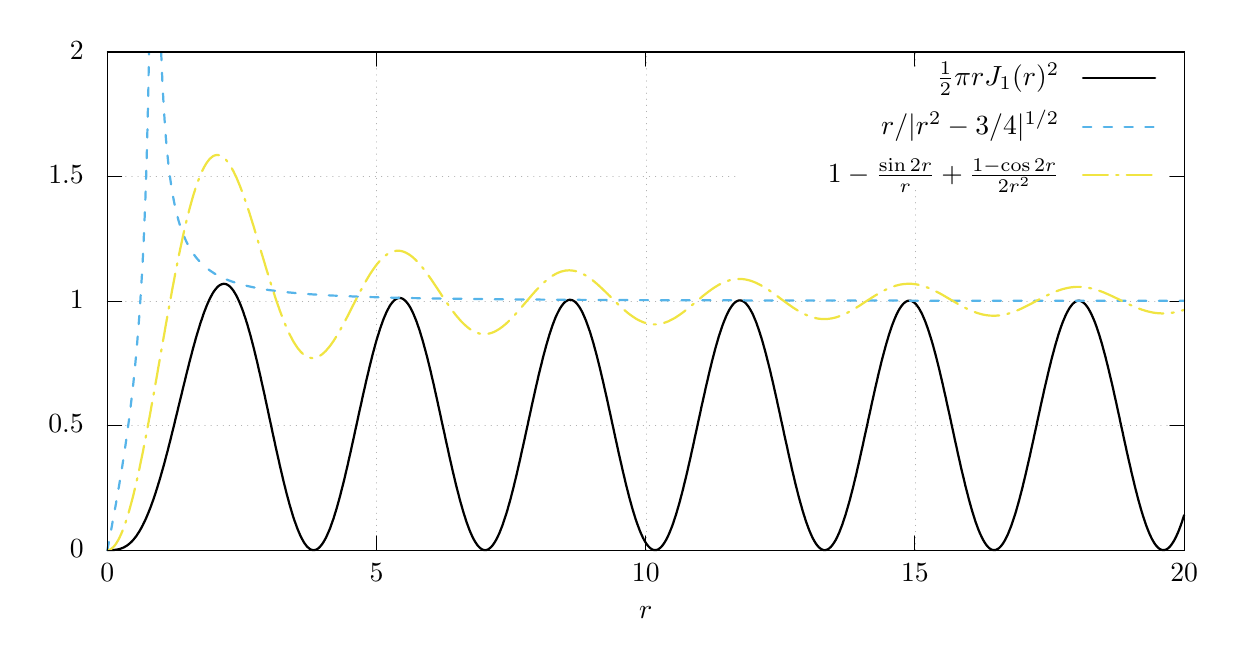
\begin{tikzpicture}[gnuplot]
	%% generated with GNUPLOT 6.0p4 (Lua 5.4; terminal rev. Jun 2020, script rev. 120)
	%% 2026/06/01 15:56:30
	\tikzset{every node/.append style={font={\normalsize}}}
	\path (0.000,0.000) rectangle (15.240,7.620);
	\gpcolor{color=gp lt color axes}
	\gpsetlinetype{gp lt axes}
	\gpsetdashtype{gp dt axes}
	\gpsetlinewidth{0.50}
	\draw[gp path] (1.012,0.985)--(14.687,0.985);
	\gpcolor{color=gp lt color border}
	\gpsetlinetype{gp lt border}
	\gpsetdashtype{gp dt solid}
	\gpsetlinewidth{1.00}
	\draw[gp path] (1.012,0.985)--(1.192,0.985);
	\draw[gp path] (14.687,0.985)--(14.507,0.985);
	\node[gp node right] at (0.828,0.985) {$0$};
	\gpcolor{color=gp lt color axes}
	\gpsetlinetype{gp lt axes}
	\gpsetdashtype{gp dt axes}
	\gpsetlinewidth{0.50}
	\draw[gp path] (1.012,2.567)--(14.687,2.567);
	\gpcolor{color=gp lt color border}
	\gpsetlinetype{gp lt border}
	\gpsetdashtype{gp dt solid}
	\gpsetlinewidth{1.00}
	\draw[gp path] (1.012,2.567)--(1.192,2.567);
	\draw[gp path] (14.687,2.567)--(14.507,2.567);
	\node[gp node right] at (0.828,2.567) {$0.5$};
	\gpcolor{color=gp lt color axes}
	\gpsetlinetype{gp lt axes}
	\gpsetdashtype{gp dt axes}
	\gpsetlinewidth{0.50}
	\draw[gp path] (1.012,4.148)--(14.687,4.148);
	\gpcolor{color=gp lt color border}
	\gpsetlinetype{gp lt border}
	\gpsetdashtype{gp dt solid}
	\gpsetlinewidth{1.00}
	\draw[gp path] (1.012,4.148)--(1.192,4.148);
	\draw[gp path] (14.687,4.148)--(14.507,4.148);
	\node[gp node right] at (0.828,4.148) {$1$};
	\gpcolor{color=gp lt color axes}
	\gpsetlinetype{gp lt axes}
	\gpsetdashtype{gp dt axes}
	\gpsetlinewidth{0.50}
	\draw[gp path] (1.012,5.730)--(8.987,5.730);
	\draw[gp path] (14.503,5.730)--(14.687,5.730);
	\gpcolor{color=gp lt color border}
	\gpsetlinetype{gp lt border}
	\gpsetdashtype{gp dt solid}
	\gpsetlinewidth{1.00}
	\draw[gp path] (1.012,5.730)--(1.192,5.730);
	\draw[gp path] (14.687,5.730)--(14.507,5.730);
	\node[gp node right] at (0.828,5.730) {$1.5$};
	\gpcolor{color=gp lt color axes}
	\gpsetlinetype{gp lt axes}
	\gpsetdashtype{gp dt axes}
	\gpsetlinewidth{0.50}
	\draw[gp path] (1.012,7.311)--(14.687,7.311);
	\gpcolor{color=gp lt color border}
	\gpsetlinetype{gp lt border}
	\gpsetdashtype{gp dt solid}
	\gpsetlinewidth{1.00}
	\draw[gp path] (1.012,7.311)--(1.192,7.311);
	\draw[gp path] (14.687,7.311)--(14.507,7.311);
	\node[gp node right] at (0.828,7.311) {$2$};
	\gpcolor{color=gp lt color axes}
	\gpsetlinetype{gp lt axes}
	\gpsetdashtype{gp dt axes}
	\gpsetlinewidth{0.50}
	\draw[gp path] (1.012,0.985)--(1.012,7.311);
	\gpcolor{color=gp lt color border}
	\gpsetlinetype{gp lt border}
	\gpsetdashtype{gp dt solid}
	\gpsetlinewidth{1.00}
	\draw[gp path] (1.012,0.985)--(1.012,1.165);
	\draw[gp path] (1.012,7.311)--(1.012,7.131);
	\node[gp node center] at (1.012,0.677) {$0$};
	\gpcolor{color=gp lt color axes}
	\gpsetlinetype{gp lt axes}
	\gpsetdashtype{gp dt axes}
	\gpsetlinewidth{0.50}
	\draw[gp path] (4.431,0.985)--(4.431,7.311);
	\gpcolor{color=gp lt color border}
	\gpsetlinetype{gp lt border}
	\gpsetdashtype{gp dt solid}
	\gpsetlinewidth{1.00}
	\draw[gp path] (4.431,0.985)--(4.431,1.165);
	\draw[gp path] (4.431,7.311)--(4.431,7.131);
	\node[gp node center] at (4.431,0.677) {$5$};
	\gpcolor{color=gp lt color axes}
	\gpsetlinetype{gp lt axes}
	\gpsetdashtype{gp dt axes}
	\gpsetlinewidth{0.50}
	\draw[gp path] (7.850,0.985)--(7.850,7.311);
	\gpcolor{color=gp lt color border}
	\gpsetlinetype{gp lt border}
	\gpsetdashtype{gp dt solid}
	\gpsetlinewidth{1.00}
	\draw[gp path] (7.850,0.985)--(7.850,1.165);
	\draw[gp path] (7.850,7.311)--(7.850,7.131);
	\node[gp node center] at (7.850,0.677) {$10$};
	\gpcolor{color=gp lt color axes}
	\gpsetlinetype{gp lt axes}
	\gpsetdashtype{gp dt axes}
	\gpsetlinewidth{0.50}
	\draw[gp path] (11.268,0.985)--(11.268,5.591);
	\draw[gp path] (11.268,7.131)--(11.268,7.311);
	\gpcolor{color=gp lt color border}
	\gpsetlinetype{gp lt border}
	\gpsetdashtype{gp dt solid}
	\gpsetlinewidth{1.00}
	\draw[gp path] (11.268,0.985)--(11.268,1.165);
	\draw[gp path] (11.268,7.311)--(11.268,7.131);
	\node[gp node center] at (11.268,0.677) {$15$};
	\gpcolor{color=gp lt color axes}
	\gpsetlinetype{gp lt axes}
	\gpsetdashtype{gp dt axes}
	\gpsetlinewidth{0.50}
	\draw[gp path] (14.687,0.985)--(14.687,7.311);
	\gpcolor{color=gp lt color border}
	\gpsetlinetype{gp lt border}
	\gpsetdashtype{gp dt solid}
	\gpsetlinewidth{1.00}
	\draw[gp path] (14.687,0.985)--(14.687,1.165);
	\draw[gp path] (14.687,7.311)--(14.687,7.131);
	\node[gp node center] at (14.687,0.677) {$20$};
	\draw[gp path] (1.012,7.311)--(1.012,0.985)--(14.687,0.985)--(14.687,7.311)--cycle;
	\node[gp node right] at (13.219,6.977) {$\frac{1}{2} \pi r \BesselJ{1}(r)^2$};
	\gpcolor{rgb color={0.000,0.000,0.000}}
	\gpsetdashtype{gp dt 1}
	\gpsetlinewidth{2.00}
	\draw[gp path] (13.403,6.977)--(14.319,6.977);
	\draw[gp path] (1.012,0.985)--(1.026,0.985)--(1.039,0.985)--(1.053,0.985)--(1.067,0.986)%
	--(1.080,0.986)--(1.094,0.987)--(1.108,0.988)--(1.122,0.990)--(1.135,0.992)--(1.149,0.995)%
	--(1.163,0.998)--(1.176,1.002)--(1.190,1.007)--(1.204,1.012)--(1.217,1.018)--(1.231,1.025)%
	--(1.245,1.033)--(1.258,1.041)--(1.272,1.051)--(1.286,1.062)--(1.299,1.073)--(1.313,1.086)%
	--(1.327,1.100)--(1.341,1.115)--(1.354,1.131)--(1.368,1.149)--(1.382,1.167)--(1.395,1.187)%
	--(1.409,1.208)--(1.423,1.231)--(1.436,1.254)--(1.450,1.279)--(1.464,1.306)--(1.477,1.333)%
	--(1.491,1.362)--(1.505,1.393)--(1.518,1.424)--(1.532,1.457)--(1.546,1.492)--(1.560,1.527)%
	--(1.573,1.564)--(1.587,1.602)--(1.601,1.641)--(1.614,1.682)--(1.628,1.724)--(1.642,1.767)%
	--(1.655,1.811)--(1.669,1.856)--(1.683,1.902)--(1.696,1.949)--(1.710,1.998)--(1.724,2.047)%
	--(1.738,2.097)--(1.751,2.148)--(1.765,2.200)--(1.779,2.252)--(1.792,2.305)--(1.806,2.359)%
	--(1.820,2.414)--(1.833,2.469)--(1.847,2.524)--(1.861,2.580)--(1.874,2.636)--(1.888,2.692)%
	--(1.902,2.749)--(1.915,2.805)--(1.929,2.862)--(1.943,2.919)--(1.957,2.975)--(1.970,3.032)%
	--(1.984,3.088)--(1.998,3.144)--(2.011,3.199)--(2.025,3.255)--(2.039,3.309)--(2.052,3.363)%
	--(2.066,3.416)--(2.080,3.469)--(2.093,3.520)--(2.107,3.571)--(2.121,3.621)--(2.134,3.669)%
	--(2.148,3.717)--(2.162,3.763)--(2.176,3.808)--(2.189,3.852)--(2.203,3.894)--(2.217,3.935)%
	--(2.230,3.975)--(2.244,4.013)--(2.258,4.049)--(2.271,4.083)--(2.285,4.116)--(2.299,4.147)%
	--(2.312,4.176)--(2.326,4.203)--(2.340,4.228)--(2.353,4.252)--(2.367,4.273)--(2.381,4.292)%
	--(2.395,4.309)--(2.408,4.324)--(2.422,4.337)--(2.436,4.347)--(2.449,4.355)--(2.463,4.361)%
	--(2.477,4.365)--(2.490,4.367)--(2.504,4.366)--(2.518,4.363)--(2.531,4.358)--(2.545,4.350)%
	--(2.559,4.340)--(2.573,4.328)--(2.586,4.314)--(2.600,4.297)--(2.614,4.278)--(2.627,4.257)%
	--(2.641,4.234)--(2.655,4.208)--(2.668,4.181)--(2.682,4.151)--(2.696,4.119)--(2.709,4.086)%
	--(2.723,4.050)--(2.737,4.012)--(2.750,3.972)--(2.764,3.931)--(2.778,3.888)--(2.792,3.843)%
	--(2.805,3.796)--(2.819,3.748)--(2.833,3.698)--(2.846,3.647)--(2.860,3.594)--(2.874,3.540)%
	--(2.887,3.485)--(2.901,3.428)--(2.915,3.371)--(2.928,3.312)--(2.942,3.252)--(2.956,3.192)%
	--(2.969,3.131)--(2.983,3.069)--(2.997,3.007)--(3.011,2.944)--(3.024,2.880)--(3.038,2.817)%
	--(3.052,2.753)--(3.065,2.689)--(3.079,2.625)--(3.093,2.561)--(3.106,2.497)--(3.120,2.433)%
	--(3.134,2.370)--(3.147,2.307)--(3.161,2.245)--(3.175,2.183)--(3.189,2.122)--(3.202,2.061)%
	--(3.216,2.002)--(3.230,1.943)--(3.243,1.886)--(3.257,1.829)--(3.271,1.774)--(3.284,1.720)%
	--(3.298,1.668)--(3.312,1.617)--(3.325,1.567)--(3.339,1.520)--(3.353,1.473)--(3.366,1.429)%
	--(3.380,1.386)--(3.394,1.345)--(3.408,1.307)--(3.421,1.270)--(3.435,1.235)--(3.449,1.202)%
	--(3.462,1.171)--(3.476,1.143)--(3.490,1.117)--(3.503,1.093)--(3.517,1.071)--(3.531,1.052)%
	--(3.544,1.035)--(3.558,1.021)--(3.572,1.009)--(3.585,0.999)--(3.599,0.992)--(3.613,0.987)%
	--(3.627,0.985)--(3.640,0.985)--(3.654,0.988)--(3.668,0.993)--(3.681,1.001)--(3.695,1.011)%
	--(3.709,1.024)--(3.722,1.039)--(3.736,1.056)--(3.750,1.076)--(3.763,1.098)--(3.777,1.122)%
	--(3.791,1.149)--(3.804,1.178)--(3.818,1.209)--(3.832,1.242)--(3.846,1.277)--(3.859,1.315)%
	--(3.873,1.354)--(3.887,1.395)--(3.900,1.438)--(3.914,1.483)--(3.928,1.529)--(3.941,1.577)%
	--(3.955,1.627)--(3.969,1.678)--(3.982,1.731)--(3.996,1.785)--(4.010,1.840)--(4.024,1.896)%
	--(4.037,1.954)--(4.051,2.012)--(4.065,2.071)--(4.078,2.132)--(4.092,2.192)--(4.106,2.254)%
	--(4.119,2.316)--(4.133,2.378)--(4.147,2.441)--(4.160,2.504)--(4.174,2.567)--(4.188,2.630)%
	--(4.201,2.693)--(4.215,2.756)--(4.229,2.818)--(4.243,2.881)--(4.256,2.943)--(4.270,3.004)%
	--(4.284,3.064)--(4.297,3.124)--(4.311,3.183)--(4.325,3.241)--(4.338,3.298)--(4.352,3.354)%
	--(4.366,3.409)--(4.379,3.463)--(4.393,3.515)--(4.407,3.566)--(4.420,3.615)--(4.434,3.663)%
	--(4.448,3.708)--(4.462,3.753)--(4.475,3.795)--(4.489,3.835)--(4.503,3.874)--(4.516,3.911)%
	--(4.530,3.945)--(4.544,3.977)--(4.557,4.008)--(4.571,4.036)--(4.585,4.061)--(4.598,4.085)%
	--(4.612,4.106)--(4.626,4.125)--(4.640,4.141)--(4.653,4.155)--(4.667,4.166)--(4.681,4.175)%
	--(4.694,4.182)--(4.708,4.186)--(4.722,4.187)--(4.735,4.186)--(4.749,4.183)--(4.763,4.177)%
	--(4.776,4.168)--(4.790,4.157)--(4.804,4.144)--(4.817,4.128)--(4.831,4.110)--(4.845,4.089)%
	--(4.859,4.066)--(4.872,4.041)--(4.886,4.013)--(4.900,3.983)--(4.913,3.951)--(4.927,3.917)%
	--(4.941,3.881)--(4.954,3.843)--(4.968,3.802)--(4.982,3.760)--(4.995,3.716)--(5.009,3.671)%
	--(5.023,3.623)--(5.036,3.574)--(5.050,3.523)--(5.064,3.471)--(5.078,3.418)--(5.091,3.363)%
	--(5.105,3.307)--(5.119,3.250)--(5.132,3.192)--(5.146,3.133)--(5.160,3.073)--(5.173,3.012)%
	--(5.187,2.950)--(5.201,2.888)--(5.214,2.826)--(5.228,2.763)--(5.242,2.700)--(5.255,2.636)%
	--(5.269,2.573)--(5.283,2.510)--(5.297,2.446)--(5.310,2.383)--(5.324,2.321)--(5.338,2.258)%
	--(5.351,2.196)--(5.365,2.135)--(5.379,2.075)--(5.392,2.015)--(5.406,1.956)--(5.420,1.898)%
	--(5.433,1.842)--(5.447,1.786)--(5.461,1.732)--(5.475,1.679)--(5.488,1.627)--(5.502,1.577)%
	--(5.516,1.529)--(5.529,1.482)--(5.543,1.437)--(5.557,1.394)--(5.570,1.352)--(5.584,1.313)%
	--(5.598,1.275)--(5.611,1.240)--(5.625,1.207)--(5.639,1.175)--(5.652,1.147)--(5.666,1.120)%
	--(5.680,1.096)--(5.694,1.074)--(5.707,1.054)--(5.721,1.037)--(5.735,1.022)--(5.748,1.010)%
	--(5.762,1.000)--(5.776,0.992)--(5.789,0.988)--(5.803,0.985)--(5.817,0.985)--(5.830,0.988)%
	--(5.844,0.993)--(5.858,1.001)--(5.871,1.011)--(5.885,1.024)--(5.899,1.039)--(5.913,1.057)%
	--(5.926,1.077)--(5.940,1.099)--(5.954,1.124)--(5.967,1.151)--(5.981,1.180)--(5.995,1.211)%
	--(6.008,1.245)--(6.022,1.280)--(6.036,1.318)--(6.049,1.358)--(6.063,1.400)--(6.077,1.443)%
	--(6.091,1.488)--(6.104,1.536)--(6.118,1.584)--(6.132,1.634)--(6.145,1.686)--(6.159,1.739)%
	--(6.173,1.794)--(6.186,1.850)--(6.200,1.906)--(6.214,1.964)--(6.227,2.023)--(6.241,2.083)%
	--(6.255,2.143)--(6.268,2.205)--(6.282,2.267)--(6.296,2.329)--(6.310,2.392)--(6.323,2.454)%
	--(6.337,2.518)--(6.351,2.581)--(6.364,2.644)--(6.378,2.707)--(6.392,2.770)--(6.405,2.833)%
	--(6.419,2.895)--(6.433,2.957)--(6.446,3.018)--(6.460,3.078)--(6.474,3.138)--(6.487,3.197)%
	--(6.501,3.254)--(6.515,3.311)--(6.529,3.366)--(6.542,3.421)--(6.556,3.474)--(6.570,3.525)%
	--(6.583,3.575)--(6.597,3.623)--(6.611,3.670)--(6.624,3.715)--(6.638,3.758)--(6.652,3.800)%
	--(6.665,3.839)--(6.679,3.876)--(6.693,3.912)--(6.706,3.945)--(6.720,3.976)--(6.734,4.004)%
	--(6.748,4.031)--(6.761,4.055)--(6.775,4.077)--(6.789,4.096)--(6.802,4.113)--(6.816,4.128)%
	--(6.830,4.140)--(6.843,4.150)--(6.857,4.157)--(6.871,4.162)--(6.884,4.164)--(6.898,4.163)%
	--(6.912,4.160)--(6.926,4.155)--(6.939,4.147)--(6.953,4.137)--(6.967,4.124)--(6.980,4.108)%
	--(6.994,4.090)--(7.008,4.070)--(7.021,4.048)--(7.035,4.023)--(7.049,3.995)--(7.062,3.966)%
	--(7.076,3.934)--(7.090,3.900)--(7.103,3.864)--(7.117,3.826)--(7.131,3.786)--(7.145,3.745)%
	--(7.158,3.701)--(7.172,3.655)--(7.186,3.608)--(7.199,3.559)--(7.213,3.508)--(7.227,3.456)%
	--(7.240,3.403)--(7.254,3.348)--(7.268,3.292)--(7.281,3.235)--(7.295,3.177)--(7.309,3.118)%
	--(7.322,3.058)--(7.336,2.998)--(7.350,2.936)--(7.364,2.874)--(7.377,2.812)--(7.391,2.749)%
	--(7.405,2.686)--(7.418,2.623)--(7.432,2.559)--(7.446,2.496)--(7.459,2.433)--(7.473,2.370)%
	--(7.487,2.307)--(7.500,2.245)--(7.514,2.183)--(7.528,2.122)--(7.542,2.062)--(7.555,2.002)%
	--(7.569,1.944)--(7.583,1.886)--(7.596,1.829)--(7.610,1.774)--(7.624,1.720)--(7.637,1.667)%
	--(7.651,1.616)--(7.665,1.566)--(7.678,1.518)--(7.692,1.472)--(7.706,1.427)--(7.719,1.384)%
	--(7.733,1.343)--(7.747,1.304)--(7.761,1.267)--(7.774,1.232)--(7.788,1.199)--(7.802,1.168)%
	--(7.815,1.140)--(7.829,1.114)--(7.843,1.090)--(7.856,1.068)--(7.870,1.049)--(7.884,1.033)%
	--(7.897,1.019)--(7.911,1.007)--(7.925,0.998)--(7.938,0.991)--(7.952,0.987)--(7.966,0.985)%
	--(7.980,0.986)--(7.993,0.989)--(8.007,0.995)--(8.021,1.004)--(8.034,1.014)--(8.048,1.028)%
	--(8.062,1.044)--(8.075,1.062)--(8.089,1.083)--(8.103,1.106)--(8.116,1.131)--(8.130,1.159)%
	--(8.144,1.189)--(8.157,1.221)--(8.171,1.255)--(8.185,1.291)--(8.199,1.330)--(8.212,1.370)%
	--(8.226,1.412)--(8.240,1.457)--(8.253,1.503)--(8.267,1.550)--(8.281,1.599)--(8.294,1.650)%
	--(8.308,1.702)--(8.322,1.756)--(8.335,1.811)--(8.349,1.867)--(8.363,1.924)--(8.377,1.983)%
	--(8.390,2.042)--(8.404,2.102)--(8.418,2.163)--(8.431,2.224)--(8.445,2.286)--(8.459,2.349)%
	--(8.472,2.412)--(8.486,2.475)--(8.500,2.538)--(8.513,2.601)--(8.527,2.665)--(8.541,2.728)%
	--(8.554,2.791)--(8.568,2.853)--(8.582,2.915)--(8.596,2.977)--(8.609,3.038)--(8.623,3.098)%
	--(8.637,3.157)--(8.650,3.215)--(8.664,3.273)--(8.678,3.329)--(8.691,3.384)--(8.705,3.437)%
	--(8.719,3.490)--(8.732,3.541)--(8.746,3.590)--(8.760,3.638)--(8.773,3.684)--(8.787,3.728)%
	--(8.801,3.770)--(8.815,3.811)--(8.828,3.849)--(8.842,3.886)--(8.856,3.920)--(8.869,3.952)%
	--(8.883,3.982)--(8.897,4.010)--(8.910,4.035)--(8.924,4.058)--(8.938,4.079)--(8.951,4.097)%
	--(8.965,4.113)--(8.979,4.127)--(8.993,4.138)--(9.006,4.146)--(9.020,4.152)--(9.034,4.156)%
	--(9.047,4.157)--(9.061,4.155)--(9.075,4.151)--(9.088,4.144)--(9.102,4.135)--(9.116,4.123)%
	--(9.129,4.109)--(9.143,4.092)--(9.157,4.073)--(9.170,4.052)--(9.184,4.028)--(9.198,4.002)%
	--(9.212,3.974)--(9.225,3.943)--(9.239,3.910)--(9.253,3.875)--(9.266,3.838)--(9.280,3.799)%
	--(9.294,3.758)--(9.307,3.715)--(9.321,3.671)--(9.335,3.624)--(9.348,3.576)--(9.362,3.526)%
	--(9.376,3.475)--(9.389,3.422)--(9.403,3.368)--(9.417,3.313)--(9.431,3.256)--(9.444,3.199)%
	--(9.458,3.140)--(9.472,3.080)--(9.485,3.020)--(9.499,2.959)--(9.513,2.897)--(9.526,2.835)%
	--(9.540,2.772)--(9.554,2.709)--(9.567,2.646)--(9.581,2.583)--(9.595,2.520)--(9.608,2.456)%
	--(9.622,2.393)--(9.636,2.331)--(9.650,2.268)--(9.663,2.206)--(9.677,2.145)--(9.691,2.084)%
	--(9.704,2.024)--(9.718,1.965)--(9.732,1.907)--(9.745,1.850)--(9.759,1.794)--(9.773,1.740)%
	--(9.786,1.687)--(9.800,1.635)--(9.814,1.584)--(9.828,1.536)--(9.841,1.488)--(9.855,1.443)%
	--(9.869,1.399)--(9.882,1.358)--(9.896,1.318)--(9.910,1.280)--(9.923,1.244)--(9.937,1.211)%
	--(9.951,1.179)--(9.964,1.150)--(9.978,1.123)--(9.992,1.098)--(10.005,1.076)--(10.019,1.056)%
	--(10.033,1.038)--(10.047,1.023)--(10.060,1.011)--(10.074,1.001)--(10.088,0.993)--(10.101,0.988)%
	--(10.115,0.985)--(10.129,0.985)--(10.142,0.988)--(10.156,0.993)--(10.170,1.000)--(10.183,1.010)%
	--(10.197,1.023)--(10.211,1.038)--(10.224,1.055)--(10.238,1.075)--(10.252,1.097)--(10.266,1.122)%
	--(10.279,1.149)--(10.293,1.178)--(10.307,1.209)--(10.320,1.243)--(10.334,1.279)--(10.348,1.316)%
	--(10.361,1.356)--(10.375,1.398)--(10.389,1.441)--(10.402,1.487)--(10.416,1.534)--(10.430,1.583)%
	--(10.444,1.633)--(10.457,1.685)--(10.471,1.738)--(10.485,1.792)--(10.498,1.848)--(10.512,1.905)%
	--(10.526,1.963)--(10.539,2.022)--(10.553,2.082)--(10.567,2.143)--(10.580,2.204)--(10.594,2.266)%
	--(10.608,2.328)--(10.621,2.391)--(10.635,2.454)--(10.649,2.517)--(10.663,2.580)--(10.676,2.644)%
	--(10.690,2.707)--(10.704,2.770)--(10.717,2.832)--(10.731,2.895)--(10.745,2.956)--(10.758,3.017)%
	--(10.772,3.078)--(10.786,3.137)--(10.799,3.196)--(10.813,3.254)--(10.827,3.310)--(10.840,3.365)%
	--(10.854,3.420)--(10.868,3.472)--(10.882,3.524)--(10.895,3.573)--(10.909,3.622)--(10.923,3.668)%
	--(10.936,3.713)--(10.950,3.756)--(10.964,3.797)--(10.977,3.836)--(10.991,3.873)--(11.005,3.908)%
	--(11.018,3.940)--(11.032,3.971)--(11.046,3.999)--(11.059,4.025)--(11.073,4.049)--(11.087,4.071)%
	--(11.101,4.090)--(11.114,4.106)--(11.128,4.120)--(11.142,4.132)--(11.155,4.141)--(11.169,4.148)%
	--(11.183,4.152)--(11.196,4.153)--(11.210,4.152)--(11.224,4.149)--(11.237,4.143)--(11.251,4.134)%
	--(11.265,4.123)--(11.279,4.110)--(11.292,4.094)--(11.306,4.075)--(11.320,4.055)--(11.333,4.031)%
	--(11.347,4.006)--(11.361,3.978)--(11.374,3.948)--(11.388,3.916)--(11.402,3.881)--(11.415,3.845)%
	--(11.429,3.806)--(11.443,3.766)--(11.456,3.723)--(11.470,3.679)--(11.484,3.633)--(11.498,3.585)%
	--(11.511,3.536)--(11.525,3.485)--(11.539,3.432)--(11.552,3.379)--(11.566,3.324)--(11.580,3.267)%
	--(11.593,3.210)--(11.607,3.152)--(11.621,3.092)--(11.634,3.032)--(11.648,2.971)--(11.662,2.910)%
	--(11.675,2.847)--(11.689,2.785)--(11.703,2.722)--(11.717,2.659)--(11.730,2.596)--(11.744,2.532)%
	--(11.758,2.469)--(11.771,2.406)--(11.785,2.343)--(11.799,2.281)--(11.812,2.218)--(11.826,2.157)%
	--(11.840,2.096)--(11.853,2.036)--(11.867,1.977)--(11.881,1.919)--(11.895,1.862)--(11.908,1.805)%
	--(11.922,1.751)--(11.936,1.697)--(11.949,1.645)--(11.963,1.594)--(11.977,1.545)--(11.990,1.498)%
	--(12.004,1.452)--(12.018,1.408)--(12.031,1.366)--(12.045,1.325)--(12.059,1.287)--(12.072,1.251)%
	--(12.086,1.217)--(12.100,1.185)--(12.114,1.155)--(12.127,1.128)--(12.141,1.103)--(12.155,1.080)%
	--(12.168,1.060)--(12.182,1.042)--(12.196,1.026)--(12.209,1.013)--(12.223,1.002)--(12.237,0.994)%
	--(12.250,0.989)--(12.264,0.986)--(12.278,0.985)--(12.291,0.987)--(12.305,0.992)--(12.319,0.999)%
	--(12.333,1.008)--(12.346,1.020)--(12.360,1.035)--(12.374,1.052)--(12.387,1.071)--(12.401,1.093)%
	--(12.415,1.117)--(12.428,1.144)--(12.442,1.172)--(12.456,1.203)--(12.469,1.237)--(12.483,1.272)%
	--(12.497,1.309)--(12.510,1.349)--(12.524,1.390)--(12.538,1.433)--(12.552,1.478)--(12.565,1.525)%
	--(12.579,1.574)--(12.593,1.624)--(12.606,1.675)--(12.620,1.728)--(12.634,1.782)--(12.647,1.838)%
	--(12.661,1.895)--(12.675,1.953)--(12.688,2.011)--(12.702,2.071)--(12.716,2.132)--(12.730,2.193)%
	--(12.743,2.255)--(12.757,2.317)--(12.771,2.380)--(12.784,2.443)--(12.798,2.506)--(12.812,2.569)%
	--(12.825,2.632)--(12.839,2.696)--(12.853,2.759)--(12.866,2.821)--(12.880,2.884)--(12.894,2.945)%
	--(12.907,3.007)--(12.921,3.067)--(12.935,3.127)--(12.949,3.185)--(12.962,3.243)--(12.976,3.300)%
	--(12.990,3.356)--(13.003,3.410)--(13.017,3.463)--(13.031,3.514)--(13.044,3.564)--(13.058,3.613)%
	--(13.072,3.659)--(13.085,3.704)--(13.099,3.748)--(13.113,3.789)--(13.126,3.828)--(13.140,3.866)%
	--(13.154,3.901)--(13.168,3.934)--(13.181,3.965)--(13.195,3.994)--(13.209,4.020)--(13.222,4.044)%
	--(13.236,4.066)--(13.250,4.085)--(13.263,4.102)--(13.277,4.117)--(13.291,4.129)--(13.304,4.138)%
	--(13.318,4.145)--(13.332,4.150)--(13.346,4.152)--(13.359,4.151)--(13.373,4.148)--(13.387,4.142)%
	--(13.400,4.134)--(13.414,4.123)--(13.428,4.110)--(13.441,4.095)--(13.455,4.076)--(13.469,4.056)%
	--(13.482,4.033)--(13.496,4.008)--(13.510,3.980)--(13.523,3.951)--(13.537,3.919)--(13.551,3.885)%
	--(13.565,3.848)--(13.578,3.810)--(13.592,3.770)--(13.606,3.728)--(13.619,3.684)--(13.633,3.638)%
	--(13.647,3.590)--(13.660,3.541)--(13.674,3.490)--(13.688,3.438)--(13.701,3.384)--(13.715,3.330)%
	--(13.729,3.273)--(13.742,3.216)--(13.756,3.158)--(13.770,3.099)--(13.784,3.039)--(13.797,2.978)%
	--(13.811,2.916)--(13.825,2.854)--(13.838,2.792)--(13.852,2.729)--(13.866,2.666)--(13.879,2.602)%
	--(13.893,2.539)--(13.907,2.476)--(13.920,2.413)--(13.934,2.350)--(13.948,2.287)--(13.961,2.225)%
	--(13.975,2.164)--(13.989,2.103)--(14.003,2.043)--(14.016,1.983)--(14.030,1.925)--(14.044,1.868)%
	--(14.057,1.811)--(14.071,1.756)--(14.085,1.703)--(14.098,1.650)--(14.112,1.600)--(14.126,1.550)%
	--(14.139,1.503)--(14.153,1.457)--(14.167,1.412)--(14.181,1.370)--(14.194,1.330)--(14.208,1.291)%
	--(14.222,1.255)--(14.235,1.221)--(14.249,1.188)--(14.263,1.158)--(14.276,1.131)--(14.290,1.105)%
	--(14.304,1.082)--(14.317,1.062)--(14.331,1.043)--(14.345,1.028)--(14.358,1.014)--(14.372,1.003)%
	--(14.386,0.995)--(14.400,0.989)--(14.413,0.986)--(14.427,0.985)--(14.441,0.987)--(14.454,0.991)%
	--(14.468,0.998)--(14.482,1.007)--(14.495,1.019)--(14.509,1.033)--(14.523,1.050)--(14.536,1.069)%
	--(14.550,1.091)--(14.564,1.115)--(14.577,1.141)--(14.591,1.169)--(14.605,1.200)--(14.619,1.233)%
	--(14.632,1.268)--(14.646,1.305)--(14.660,1.345)--(14.673,1.386)--(14.687,1.429);
	\gpcolor{color=gp lt color border}
	\node[gp node right] at (13.219,6.669) { };
	\gpcolor{color=gpbgfillcolor}
	\gpsetlinetype{gp lt plot 4}
	\gpsetdashtype{gp dt solid}
	\gpsetlinewidth{1.00}
	\draw[gp path] (13.403,6.669)--(14.319,6.669);
	\gpcolor{color=gp lt color border}
	\node[gp node right] at (13.219,6.361) {$r/\abs{r^2 - 3/4}^{1/2}$};
	\gpcolor{rgb color={0.337,0.706,0.914}}
	\gpsetlinetype{gp lt border}
	\gpsetdashtype{gp dt 3}
	\gpsetlinewidth{2.00}
	\draw[gp path] (13.403,6.361)--(14.319,6.361);
	\draw[gp path] (1.012,0.985)--(1.026,1.058)--(1.039,1.131)--(1.053,1.205)--(1.067,1.279)%
	--(1.080,1.353)--(1.094,1.428)--(1.108,1.504)--(1.122,1.580)--(1.135,1.658)--(1.149,1.737)%
	--(1.163,1.817)--(1.176,1.898)--(1.190,1.982)--(1.204,2.067)--(1.217,2.154)--(1.231,2.244)%
	--(1.245,2.337)--(1.258,2.432)--(1.272,2.531)--(1.286,2.634)--(1.299,2.741)--(1.313,2.853)%
	--(1.327,2.971)--(1.341,3.094)--(1.354,3.225)--(1.368,3.364)--(1.382,3.512)--(1.395,3.671)%
	--(1.409,3.843)--(1.423,4.030)--(1.436,4.235)--(1.450,4.462)--(1.464,4.717)--(1.477,5.006)%
	--(1.491,5.340)--(1.505,5.733)--(1.518,6.207)--(1.532,6.800)--(1.541,7.311);
	\draw[gp path] (1.695,7.311)--(1.696,7.292)--(1.710,6.956)--(1.724,6.685)--(1.738,6.459)%
	--(1.751,6.269)--(1.765,6.107)--(1.779,5.966)--(1.792,5.842)--(1.806,5.733)--(1.820,5.636)%
	--(1.833,5.549)--(1.847,5.471)--(1.861,5.400)--(1.874,5.336)--(1.888,5.277)--(1.902,5.223)%
	--(1.915,5.173)--(1.929,5.127)--(1.943,5.084)--(1.957,5.045)--(1.970,5.008)--(1.984,4.974)%
	--(1.998,4.942)--(2.011,4.912)--(2.025,4.883)--(2.039,4.857)--(2.052,4.832)--(2.066,4.808)%
	--(2.080,4.786)--(2.093,4.765)--(2.107,4.745)--(2.121,4.726)--(2.134,4.708)--(2.148,4.691)%
	--(2.162,4.675)--(2.176,4.659)--(2.189,4.645)--(2.203,4.631)--(2.217,4.617)--(2.230,4.604)%
	--(2.244,4.592)--(2.258,4.580)--(2.271,4.569)--(2.285,4.558)--(2.299,4.548)--(2.312,4.538)%
	--(2.326,4.528)--(2.340,4.519)--(2.353,4.510)--(2.367,4.501)--(2.381,4.493)--(2.395,4.485)%
	--(2.408,4.478)--(2.422,4.470)--(2.436,4.463)--(2.449,4.456)--(2.463,4.450)--(2.477,4.443)%
	--(2.490,4.437)--(2.504,4.431)--(2.518,4.425)--(2.531,4.420)--(2.545,4.414)--(2.559,4.409)%
	--(2.573,4.404)--(2.586,4.399)--(2.600,4.394)--(2.614,4.389)--(2.627,4.385)--(2.641,4.380)%
	--(2.655,4.376)--(2.668,4.372)--(2.682,4.368)--(2.696,4.364)--(2.709,4.360)--(2.723,4.356)%
	--(2.737,4.353)--(2.750,4.349)--(2.764,4.346)--(2.778,4.342)--(2.792,4.339)--(2.805,4.336)%
	--(2.819,4.333)--(2.833,4.330)--(2.846,4.327)--(2.860,4.324)--(2.874,4.321)--(2.887,4.319)%
	--(2.901,4.316)--(2.915,4.313)--(2.928,4.311)--(2.942,4.308)--(2.956,4.306)--(2.969,4.303)%
	--(2.983,4.301)--(2.997,4.299)--(3.011,4.297)--(3.024,4.295)--(3.038,4.292)--(3.052,4.290)%
	--(3.065,4.288)--(3.079,4.286)--(3.093,4.284)--(3.106,4.283)--(3.120,4.281)--(3.134,4.279)%
	--(3.147,4.277)--(3.161,4.275)--(3.175,4.274)--(3.189,4.272)--(3.202,4.270)--(3.216,4.269)%
	--(3.230,4.267)--(3.243,4.266)--(3.257,4.264)--(3.271,4.263)--(3.284,4.261)--(3.298,4.260)%
	--(3.312,4.258)--(3.325,4.257)--(3.339,4.256)--(3.353,4.254)--(3.366,4.253)--(3.380,4.252)%
	--(3.394,4.251)--(3.408,4.249)--(3.421,4.248)--(3.435,4.247)--(3.449,4.246)--(3.462,4.245)%
	--(3.476,4.243)--(3.490,4.242)--(3.503,4.241)--(3.517,4.240)--(3.531,4.239)--(3.544,4.238)%
	--(3.558,4.237)--(3.572,4.236)--(3.585,4.235)--(3.599,4.234)--(3.613,4.233)--(3.627,4.232)%
	--(3.640,4.231)--(3.654,4.231)--(3.668,4.230)--(3.681,4.229)--(3.695,4.228)--(3.709,4.227)%
	--(3.722,4.226)--(3.736,4.225)--(3.750,4.225)--(3.763,4.224)--(3.777,4.223)--(3.791,4.222)%
	--(3.804,4.222)--(3.818,4.221)--(3.832,4.220)--(3.846,4.219)--(3.859,4.219)--(3.873,4.218)%
	--(3.887,4.217)--(3.900,4.217)--(3.914,4.216)--(3.928,4.215)--(3.941,4.215)--(3.955,4.214)%
	--(3.969,4.213)--(3.982,4.213)--(3.996,4.212)--(4.010,4.212)--(4.024,4.211)--(4.037,4.210)%
	--(4.051,4.210)--(4.065,4.209)--(4.078,4.209)--(4.092,4.208)--(4.106,4.208)--(4.119,4.207)%
	--(4.133,4.207)--(4.147,4.206)--(4.160,4.205)--(4.174,4.205)--(4.188,4.204)--(4.201,4.204)%
	--(4.215,4.203)--(4.229,4.203)--(4.243,4.203)--(4.256,4.202)--(4.270,4.202)--(4.284,4.201)%
	--(4.297,4.201)--(4.311,4.200)--(4.325,4.200)--(4.338,4.199)--(4.352,4.199)--(4.366,4.198)%
	--(4.379,4.198)--(4.393,4.198)--(4.407,4.197)--(4.420,4.197)--(4.434,4.196)--(4.448,4.196)%
	--(4.462,4.196)--(4.475,4.195)--(4.489,4.195)--(4.503,4.195)--(4.516,4.194)--(4.530,4.194)%
	--(4.544,4.193)--(4.557,4.193)--(4.571,4.193)--(4.585,4.192)--(4.598,4.192)--(4.612,4.192)%
	--(4.626,4.191)--(4.640,4.191)--(4.653,4.191)--(4.667,4.190)--(4.681,4.190)--(4.694,4.190)%
	--(4.708,4.189)--(4.722,4.189)--(4.735,4.189)--(4.749,4.188)--(4.763,4.188)--(4.776,4.188)%
	--(4.790,4.188)--(4.804,4.187)--(4.817,4.187)--(4.831,4.187)--(4.845,4.186)--(4.859,4.186)%
	--(4.872,4.186)--(4.886,4.186)--(4.900,4.185)--(4.913,4.185)--(4.927,4.185)--(4.941,4.185)%
	--(4.954,4.184)--(4.968,4.184)--(4.982,4.184)--(4.995,4.184)--(5.009,4.183)--(5.023,4.183)%
	--(5.036,4.183)--(5.050,4.183)--(5.064,4.182)--(5.078,4.182)--(5.091,4.182)--(5.105,4.182)%
	--(5.119,4.181)--(5.132,4.181)--(5.146,4.181)--(5.160,4.181)--(5.173,4.181)--(5.187,4.180)%
	--(5.201,4.180)--(5.214,4.180)--(5.228,4.180)--(5.242,4.179)--(5.255,4.179)--(5.269,4.179)%
	--(5.283,4.179)--(5.297,4.179)--(5.310,4.178)--(5.324,4.178)--(5.338,4.178)--(5.351,4.178)%
	--(5.365,4.178)--(5.379,4.177)--(5.392,4.177)--(5.406,4.177)--(5.420,4.177)--(5.433,4.177)%
	--(5.447,4.177)--(5.461,4.176)--(5.475,4.176)--(5.488,4.176)--(5.502,4.176)--(5.516,4.176)%
	--(5.529,4.176)--(5.543,4.175)--(5.557,4.175)--(5.570,4.175)--(5.584,4.175)--(5.598,4.175)%
	--(5.611,4.175)--(5.625,4.174)--(5.639,4.174)--(5.652,4.174)--(5.666,4.174)--(5.680,4.174)%
	--(5.694,4.174)--(5.707,4.173)--(5.721,4.173)--(5.735,4.173)--(5.748,4.173)--(5.762,4.173)%
	--(5.776,4.173)--(5.789,4.173)--(5.803,4.172)--(5.817,4.172)--(5.830,4.172)--(5.844,4.172)%
	--(5.858,4.172)--(5.871,4.172)--(5.885,4.172)--(5.899,4.171)--(5.913,4.171)--(5.926,4.171)%
	--(5.940,4.171)--(5.954,4.171)--(5.967,4.171)--(5.981,4.171)--(5.995,4.171)--(6.008,4.170)%
	--(6.022,4.170)--(6.036,4.170)--(6.049,4.170)--(6.063,4.170)--(6.077,4.170)--(6.091,4.170)%
	--(6.104,4.170)--(6.118,4.169)--(6.132,4.169)--(6.145,4.169)--(6.159,4.169)--(6.173,4.169)%
	--(6.186,4.169)--(6.200,4.169)--(6.214,4.169)--(6.227,4.169)--(6.241,4.168)--(6.255,4.168)%
	--(6.268,4.168)--(6.282,4.168)--(6.296,4.168)--(6.310,4.168)--(6.323,4.168)--(6.337,4.168)%
	--(6.351,4.168)--(6.364,4.168)--(6.378,4.167)--(6.392,4.167)--(6.405,4.167)--(6.419,4.167)%
	--(6.433,4.167)--(6.446,4.167)--(6.460,4.167)--(6.474,4.167)--(6.487,4.167)--(6.501,4.167)%
	--(6.515,4.166)--(6.529,4.166)--(6.542,4.166)--(6.556,4.166)--(6.570,4.166)--(6.583,4.166)%
	--(6.597,4.166)--(6.611,4.166)--(6.624,4.166)--(6.638,4.166)--(6.652,4.166)--(6.665,4.165)%
	--(6.679,4.165)--(6.693,4.165)--(6.706,4.165)--(6.720,4.165)--(6.734,4.165)--(6.748,4.165)%
	--(6.761,4.165)--(6.775,4.165)--(6.789,4.165)--(6.802,4.165)--(6.816,4.165)--(6.830,4.165)%
	--(6.843,4.164)--(6.857,4.164)--(6.871,4.164)--(6.884,4.164)--(6.898,4.164)--(6.912,4.164)%
	--(6.926,4.164)--(6.939,4.164)--(6.953,4.164)--(6.967,4.164)--(6.980,4.164)--(6.994,4.164)%
	--(7.008,4.164)--(7.021,4.163)--(7.035,4.163)--(7.049,4.163)--(7.062,4.163)--(7.076,4.163)%
	--(7.090,4.163)--(7.103,4.163)--(7.117,4.163)--(7.131,4.163)--(7.145,4.163)--(7.158,4.163)%
	--(7.172,4.163)--(7.186,4.163)--(7.199,4.163)--(7.213,4.163)--(7.227,4.162)--(7.240,4.162)%
	--(7.254,4.162)--(7.268,4.162)--(7.281,4.162)--(7.295,4.162)--(7.309,4.162)--(7.322,4.162)%
	--(7.336,4.162)--(7.350,4.162)--(7.364,4.162)--(7.377,4.162)--(7.391,4.162)--(7.405,4.162)%
	--(7.418,4.162)--(7.432,4.162)--(7.446,4.161)--(7.459,4.161)--(7.473,4.161)--(7.487,4.161)%
	--(7.500,4.161)--(7.514,4.161)--(7.528,4.161)--(7.542,4.161)--(7.555,4.161)--(7.569,4.161)%
	--(7.583,4.161)--(7.596,4.161)--(7.610,4.161)--(7.624,4.161)--(7.637,4.161)--(7.651,4.161)%
	--(7.665,4.161)--(7.678,4.161)--(7.692,4.161)--(7.706,4.160)--(7.719,4.160)--(7.733,4.160)%
	--(7.747,4.160)--(7.761,4.160)--(7.774,4.160)--(7.788,4.160)--(7.802,4.160)--(7.815,4.160)%
	--(7.829,4.160)--(7.843,4.160)--(7.856,4.160)--(7.870,4.160)--(7.884,4.160)--(7.897,4.160)%
	--(7.911,4.160)--(7.925,4.160)--(7.938,4.160)--(7.952,4.160)--(7.966,4.160)--(7.980,4.159)%
	--(7.993,4.159)--(8.007,4.159)--(8.021,4.159)--(8.034,4.159)--(8.048,4.159)--(8.062,4.159)%
	--(8.075,4.159)--(8.089,4.159)--(8.103,4.159)--(8.116,4.159)--(8.130,4.159)--(8.144,4.159)%
	--(8.157,4.159)--(8.171,4.159)--(8.185,4.159)--(8.199,4.159)--(8.212,4.159)--(8.226,4.159)%
	--(8.240,4.159)--(8.253,4.159)--(8.267,4.159)--(8.281,4.159)--(8.294,4.159)--(8.308,4.158)%
	--(8.322,4.158)--(8.335,4.158)--(8.349,4.158)--(8.363,4.158)--(8.377,4.158)--(8.390,4.158)%
	--(8.404,4.158)--(8.418,4.158)--(8.431,4.158)--(8.445,4.158)--(8.459,4.158)--(8.472,4.158)%
	--(8.486,4.158)--(8.500,4.158)--(8.513,4.158)--(8.527,4.158)--(8.541,4.158)--(8.554,4.158)%
	--(8.568,4.158)--(8.582,4.158)--(8.596,4.158)--(8.609,4.158)--(8.623,4.158)--(8.637,4.158)%
	--(8.650,4.158)--(8.664,4.158)--(8.678,4.157)--(8.691,4.157)--(8.705,4.157)--(8.719,4.157)%
	--(8.732,4.157)--(8.746,4.157)--(8.760,4.157)--(8.773,4.157)--(8.787,4.157)--(8.801,4.157)%
	--(8.815,4.157)--(8.828,4.157)--(8.842,4.157)--(8.856,4.157)--(8.869,4.157)--(8.883,4.157)%
	--(8.897,4.157)--(8.910,4.157)--(8.924,4.157)--(8.938,4.157)--(8.951,4.157)--(8.965,4.157)%
	--(8.979,4.157)--(8.993,4.157)--(9.006,4.157)--(9.020,4.157)--(9.034,4.157)--(9.047,4.157)%
	--(9.061,4.157)--(9.075,4.157)--(9.088,4.157)--(9.102,4.157)--(9.116,4.156)--(9.129,4.156)%
	--(9.143,4.156)--(9.157,4.156)--(9.170,4.156)--(9.184,4.156)--(9.198,4.156)--(9.212,4.156)%
	--(9.225,4.156)--(9.239,4.156)--(9.253,4.156)--(9.266,4.156)--(9.280,4.156)--(9.294,4.156)%
	--(9.307,4.156)--(9.321,4.156)--(9.335,4.156)--(9.348,4.156)--(9.362,4.156)--(9.376,4.156)%
	--(9.389,4.156)--(9.403,4.156)--(9.417,4.156)--(9.431,4.156)--(9.444,4.156)--(9.458,4.156)%
	--(9.472,4.156)--(9.485,4.156)--(9.499,4.156)--(9.513,4.156)--(9.526,4.156)--(9.540,4.156)%
	--(9.554,4.156)--(9.567,4.156)--(9.581,4.156)--(9.595,4.156)--(9.608,4.156)--(9.622,4.156)%
	--(9.636,4.155)--(9.650,4.155)--(9.663,4.155)--(9.677,4.155)--(9.691,4.155)--(9.704,4.155)%
	--(9.718,4.155)--(9.732,4.155)--(9.745,4.155)--(9.759,4.155)--(9.773,4.155)--(9.786,4.155)%
	--(9.800,4.155)--(9.814,4.155)--(9.828,4.155)--(9.841,4.155)--(9.855,4.155)--(9.869,4.155)%
	--(9.882,4.155)--(9.896,4.155)--(9.910,4.155)--(9.923,4.155)--(9.937,4.155)--(9.951,4.155)%
	--(9.964,4.155)--(9.978,4.155)--(9.992,4.155)--(10.005,4.155)--(10.019,4.155)--(10.033,4.155)%
	--(10.047,4.155)--(10.060,4.155)--(10.074,4.155)--(10.088,4.155)--(10.101,4.155)--(10.115,4.155)%
	--(10.129,4.155)--(10.142,4.155)--(10.156,4.155)--(10.170,4.155)--(10.183,4.155)--(10.197,4.155)%
	--(10.211,4.155)--(10.224,4.155)--(10.238,4.155)--(10.252,4.155)--(10.266,4.154)--(10.279,4.154)%
	--(10.293,4.154)--(10.307,4.154)--(10.320,4.154)--(10.334,4.154)--(10.348,4.154)--(10.361,4.154)%
	--(10.375,4.154)--(10.389,4.154)--(10.402,4.154)--(10.416,4.154)--(10.430,4.154)--(10.444,4.154)%
	--(10.457,4.154)--(10.471,4.154)--(10.485,4.154)--(10.498,4.154)--(10.512,4.154)--(10.526,4.154)%
	--(10.539,4.154)--(10.553,4.154)--(10.567,4.154)--(10.580,4.154)--(10.594,4.154)--(10.608,4.154)%
	--(10.621,4.154)--(10.635,4.154)--(10.649,4.154)--(10.663,4.154)--(10.676,4.154)--(10.690,4.154)%
	--(10.704,4.154)--(10.717,4.154)--(10.731,4.154)--(10.745,4.154)--(10.758,4.154)--(10.772,4.154)%
	--(10.786,4.154)--(10.799,4.154)--(10.813,4.154)--(10.827,4.154)--(10.840,4.154)--(10.854,4.154)%
	--(10.868,4.154)--(10.882,4.154)--(10.895,4.154)--(10.909,4.154)--(10.923,4.154)--(10.936,4.154)%
	--(10.950,4.154)--(10.964,4.154)--(10.977,4.154)--(10.991,4.154)--(11.005,4.154)--(11.018,4.154)%
	--(11.032,4.154)--(11.046,4.154)--(11.059,4.154)--(11.073,4.153)--(11.087,4.153)--(11.101,4.153)%
	--(11.114,4.153)--(11.128,4.153)--(11.142,4.153)--(11.155,4.153)--(11.169,4.153)--(11.183,4.153)%
	--(11.196,4.153)--(11.210,4.153)--(11.224,4.153)--(11.237,4.153)--(11.251,4.153)--(11.265,4.153)%
	--(11.279,4.153)--(11.292,4.153)--(11.306,4.153)--(11.320,4.153)--(11.333,4.153)--(11.347,4.153)%
	--(11.361,4.153)--(11.374,4.153)--(11.388,4.153)--(11.402,4.153)--(11.415,4.153)--(11.429,4.153)%
	--(11.443,4.153)--(11.456,4.153)--(11.470,4.153)--(11.484,4.153)--(11.498,4.153)--(11.511,4.153)%
	--(11.525,4.153)--(11.539,4.153)--(11.552,4.153)--(11.566,4.153)--(11.580,4.153)--(11.593,4.153)%
	--(11.607,4.153)--(11.621,4.153)--(11.634,4.153)--(11.648,4.153)--(11.662,4.153)--(11.675,4.153)%
	--(11.689,4.153)--(11.703,4.153)--(11.717,4.153)--(11.730,4.153)--(11.744,4.153)--(11.758,4.153)%
	--(11.771,4.153)--(11.785,4.153)--(11.799,4.153)--(11.812,4.153)--(11.826,4.153)--(11.840,4.153)%
	--(11.853,4.153)--(11.867,4.153)--(11.881,4.153)--(11.895,4.153)--(11.908,4.153)--(11.922,4.153)%
	--(11.936,4.153)--(11.949,4.153)--(11.963,4.153)--(11.977,4.153)--(11.990,4.153)--(12.004,4.153)%
	--(12.018,4.153)--(12.031,4.153)--(12.045,4.153)--(12.059,4.153)--(12.072,4.153)--(12.086,4.153)%
	--(12.100,4.153)--(12.114,4.153)--(12.127,4.152)--(12.141,4.152)--(12.155,4.152)--(12.168,4.152)%
	--(12.182,4.152)--(12.196,4.152)--(12.209,4.152)--(12.223,4.152)--(12.237,4.152)--(12.250,4.152)%
	--(12.264,4.152)--(12.278,4.152)--(12.291,4.152)--(12.305,4.152)--(12.319,4.152)--(12.333,4.152)%
	--(12.346,4.152)--(12.360,4.152)--(12.374,4.152)--(12.387,4.152)--(12.401,4.152)--(12.415,4.152)%
	--(12.428,4.152)--(12.442,4.152)--(12.456,4.152)--(12.469,4.152)--(12.483,4.152)--(12.497,4.152)%
	--(12.510,4.152)--(12.524,4.152)--(12.538,4.152)--(12.552,4.152)--(12.565,4.152)--(12.579,4.152)%
	--(12.593,4.152)--(12.606,4.152)--(12.620,4.152)--(12.634,4.152)--(12.647,4.152)--(12.661,4.152)%
	--(12.675,4.152)--(12.688,4.152)--(12.702,4.152)--(12.716,4.152)--(12.730,4.152)--(12.743,4.152)%
	--(12.757,4.152)--(12.771,4.152)--(12.784,4.152)--(12.798,4.152)--(12.812,4.152)--(12.825,4.152)%
	--(12.839,4.152)--(12.853,4.152)--(12.866,4.152)--(12.880,4.152)--(12.894,4.152)--(12.907,4.152)%
	--(12.921,4.152)--(12.935,4.152)--(12.949,4.152)--(12.962,4.152)--(12.976,4.152)--(12.990,4.152)%
	--(13.003,4.152)--(13.017,4.152)--(13.031,4.152)--(13.044,4.152)--(13.058,4.152)--(13.072,4.152)%
	--(13.085,4.152)--(13.099,4.152)--(13.113,4.152)--(13.126,4.152)--(13.140,4.152)--(13.154,4.152)%
	--(13.168,4.152)--(13.181,4.152)--(13.195,4.152)--(13.209,4.152)--(13.222,4.152)--(13.236,4.152)%
	--(13.250,4.152)--(13.263,4.152)--(13.277,4.152)--(13.291,4.152)--(13.304,4.152)--(13.318,4.152)%
	--(13.332,4.152)--(13.346,4.152)--(13.359,4.152)--(13.373,4.152)--(13.387,4.152)--(13.400,4.152)%
	--(13.414,4.152)--(13.428,4.152)--(13.441,4.152)--(13.455,4.152)--(13.469,4.152)--(13.482,4.152)%
	--(13.496,4.152)--(13.510,4.152)--(13.523,4.152)--(13.537,4.152)--(13.551,4.152)--(13.565,4.152)%
	--(13.578,4.152)--(13.592,4.152)--(13.606,4.152)--(13.619,4.151)--(13.633,4.151)--(13.647,4.151)%
	--(13.660,4.151)--(13.674,4.151)--(13.688,4.151)--(13.701,4.151)--(13.715,4.151)--(13.729,4.151)%
	--(13.742,4.151)--(13.756,4.151)--(13.770,4.151)--(13.784,4.151)--(13.797,4.151)--(13.811,4.151)%
	--(13.825,4.151)--(13.838,4.151)--(13.852,4.151)--(13.866,4.151)--(13.879,4.151)--(13.893,4.151)%
	--(13.907,4.151)--(13.920,4.151)--(13.934,4.151)--(13.948,4.151)--(13.961,4.151)--(13.975,4.151)%
	--(13.989,4.151)--(14.003,4.151)--(14.016,4.151)--(14.030,4.151)--(14.044,4.151)--(14.057,4.151)%
	--(14.071,4.151)--(14.085,4.151)--(14.098,4.151)--(14.112,4.151)--(14.126,4.151)--(14.139,4.151)%
	--(14.153,4.151)--(14.167,4.151)--(14.181,4.151)--(14.194,4.151)--(14.208,4.151)--(14.222,4.151)%
	--(14.235,4.151)--(14.249,4.151)--(14.263,4.151)--(14.276,4.151)--(14.290,4.151)--(14.304,4.151)%
	--(14.317,4.151)--(14.331,4.151)--(14.345,4.151)--(14.358,4.151)--(14.372,4.151)--(14.386,4.151)%
	--(14.400,4.151)--(14.413,4.151)--(14.427,4.151)--(14.441,4.151)--(14.454,4.151)--(14.468,4.151)%
	--(14.482,4.151)--(14.495,4.151)--(14.509,4.151)--(14.523,4.151)--(14.536,4.151)--(14.550,4.151)%
	--(14.564,4.151)--(14.577,4.151)--(14.591,4.151)--(14.605,4.151)--(14.619,4.151)--(14.632,4.151)%
	--(14.646,4.151)--(14.660,4.151)--(14.673,4.151)--(14.687,4.151);
	\gpcolor{color=gp lt color border}
	\node[gp node right] at (13.219,6.053) { };
	\gpcolor{color=gpbgfillcolor}
	\gpsetlinetype{gp lt plot 4}
	\gpsetdashtype{gp dt solid}
	\gpsetlinewidth{1.00}
	\draw[gp path] (13.403,6.053)--(14.319,6.053);
	\gpcolor{color=gp lt color border}
	\node[gp node right] at (13.219,5.745) {$1 - \frac{\sin{2r}}{r} + \frac{1 - \cos{2r}}{2r^2}$};
	\gpcolor{rgb color={0.941,0.894,0.259}}
	\gpsetlinetype{gp lt border}
	\gpsetdashtype{gp dt 5}
	\gpsetlinewidth{2.00}
	\draw[gp path] (13.403,5.745)--(14.319,5.745);
	\draw[gp path] (1.026,0.986)--(1.039,0.990)--(1.053,0.996)--(1.067,1.005)--(1.080,1.017)%
	--(1.094,1.030)--(1.108,1.047)--(1.122,1.066)--(1.135,1.087)--(1.149,1.111)--(1.163,1.137)%
	--(1.176,1.165)--(1.190,1.196)--(1.204,1.229)--(1.217,1.265)--(1.231,1.302)--(1.245,1.342)%
	--(1.258,1.384)--(1.272,1.428)--(1.286,1.474)--(1.299,1.522)--(1.313,1.573)--(1.327,1.625)%
	--(1.341,1.679)--(1.354,1.734)--(1.368,1.792)--(1.382,1.851)--(1.395,1.912)--(1.409,1.974)%
	--(1.423,2.038)--(1.436,2.103)--(1.450,2.170)--(1.464,2.237)--(1.477,2.306)--(1.491,2.377)%
	--(1.505,2.448)--(1.518,2.520)--(1.532,2.593)--(1.546,2.667)--(1.560,2.742)--(1.573,2.818)%
	--(1.587,2.894)--(1.601,2.970)--(1.614,3.048)--(1.628,3.125)--(1.642,3.203)--(1.655,3.281)%
	--(1.669,3.359)--(1.683,3.437)--(1.696,3.515)--(1.710,3.594)--(1.724,3.672)--(1.738,3.749)%
	--(1.751,3.827)--(1.765,3.904)--(1.779,3.980)--(1.792,4.056)--(1.806,4.132)--(1.820,4.206)%
	--(1.833,4.280)--(1.847,4.353)--(1.861,4.425)--(1.874,4.497)--(1.888,4.567)--(1.902,4.636)%
	--(1.915,4.704)--(1.929,4.770)--(1.943,4.836)--(1.957,4.900)--(1.970,4.963)--(1.984,5.024)%
	--(1.998,5.084)--(2.011,5.142)--(2.025,5.198)--(2.039,5.253)--(2.052,5.306)--(2.066,5.358)%
	--(2.080,5.408)--(2.093,5.455)--(2.107,5.502)--(2.121,5.546)--(2.134,5.588)--(2.148,5.628)%
	--(2.162,5.666)--(2.176,5.703)--(2.189,5.737)--(2.203,5.769)--(2.217,5.800)--(2.230,5.828)%
	--(2.244,5.854)--(2.258,5.878)--(2.271,5.900)--(2.285,5.919)--(2.299,5.937)--(2.312,5.953)%
	--(2.326,5.966)--(2.340,5.977)--(2.353,5.987)--(2.367,5.994)--(2.381,5.999)--(2.395,6.002)%
	--(2.408,6.003)--(2.422,6.002)--(2.436,5.999)--(2.449,5.995)--(2.463,5.988)--(2.477,5.979)%
	--(2.490,5.968)--(2.504,5.956)--(2.518,5.942)--(2.531,5.926)--(2.545,5.908)--(2.559,5.888)%
	--(2.573,5.867)--(2.586,5.844)--(2.600,5.820)--(2.614,5.794)--(2.627,5.767)--(2.641,5.738)%
	--(2.655,5.708)--(2.668,5.676)--(2.682,5.643)--(2.696,5.609)--(2.709,5.574)--(2.723,5.538)%
	--(2.737,5.501)--(2.750,5.462)--(2.764,5.423)--(2.778,5.383)--(2.792,5.342)--(2.805,5.300)%
	--(2.819,5.258)--(2.833,5.214)--(2.846,5.171)--(2.860,5.127)--(2.874,5.082)--(2.887,5.037)%
	--(2.901,4.991)--(2.915,4.946)--(2.928,4.900)--(2.942,4.854)--(2.956,4.808)--(2.969,4.762)%
	--(2.983,4.716)--(2.997,4.670)--(3.011,4.624)--(3.024,4.578)--(3.038,4.533)--(3.052,4.488)%
	--(3.065,4.443)--(3.079,4.399)--(3.093,4.355)--(3.106,4.312)--(3.120,4.269)--(3.134,4.227)%
	--(3.147,4.186)--(3.161,4.145)--(3.175,4.105)--(3.189,4.066)--(3.202,4.028)--(3.216,3.991)%
	--(3.230,3.954)--(3.243,3.919)--(3.257,3.884)--(3.271,3.851)--(3.284,3.819)--(3.298,3.788)%
	--(3.312,3.758)--(3.325,3.729)--(3.339,3.702)--(3.353,3.675)--(3.366,3.650)--(3.380,3.626)%
	--(3.394,3.604)--(3.408,3.582)--(3.421,3.562)--(3.435,3.544)--(3.449,3.527)--(3.462,3.511)%
	--(3.476,3.496)--(3.490,3.483)--(3.503,3.471)--(3.517,3.460)--(3.531,3.451)--(3.544,3.443)%
	--(3.558,3.437)--(3.572,3.432)--(3.585,3.428)--(3.599,3.425)--(3.613,3.424)--(3.627,3.424)%
	--(3.640,3.426)--(3.654,3.428)--(3.668,3.432)--(3.681,3.438)--(3.695,3.444)--(3.709,3.452)%
	--(3.722,3.460)--(3.736,3.470)--(3.750,3.481)--(3.763,3.493)--(3.777,3.506)--(3.791,3.520)%
	--(3.804,3.536)--(3.818,3.552)--(3.832,3.569)--(3.846,3.586)--(3.859,3.605)--(3.873,3.625)%
	--(3.887,3.645)--(3.900,3.666)--(3.914,3.688)--(3.928,3.710)--(3.941,3.733)--(3.955,3.756)%
	--(3.969,3.781)--(3.982,3.805)--(3.996,3.830)--(4.010,3.855)--(4.024,3.881)--(4.037,3.907)%
	--(4.051,3.934)--(4.065,3.960)--(4.078,3.987)--(4.092,4.014)--(4.106,4.041)--(4.119,4.068)%
	--(4.133,4.095)--(4.147,4.122)--(4.160,4.149)--(4.174,4.175)--(4.188,4.202)--(4.201,4.228)%
	--(4.215,4.255)--(4.229,4.281)--(4.243,4.306)--(4.256,4.331)--(4.270,4.356)--(4.284,4.381)%
	--(4.297,4.405)--(4.311,4.428)--(4.325,4.451)--(4.338,4.474)--(4.352,4.496)--(4.366,4.517)%
	--(4.379,4.537)--(4.393,4.557)--(4.407,4.577)--(4.420,4.595)--(4.434,4.613)--(4.448,4.630)%
	--(4.462,4.646)--(4.475,4.661)--(4.489,4.676)--(4.503,4.690)--(4.516,4.703)--(4.530,4.715)%
	--(4.544,4.726)--(4.557,4.736)--(4.571,4.745)--(4.585,4.754)--(4.598,4.761)--(4.612,4.768)%
	--(4.626,4.773)--(4.640,4.778)--(4.653,4.782)--(4.667,4.784)--(4.681,4.786)--(4.694,4.787)%
	--(4.708,4.787)--(4.722,4.786)--(4.735,4.785)--(4.749,4.782)--(4.763,4.778)--(4.776,4.774)%
	--(4.790,4.768)--(4.804,4.762)--(4.817,4.755)--(4.831,4.747)--(4.845,4.739)--(4.859,4.729)%
	--(4.872,4.719)--(4.886,4.708)--(4.900,4.696)--(4.913,4.684)--(4.927,4.671)--(4.941,4.657)%
	--(4.954,4.643)--(4.968,4.628)--(4.982,4.612)--(4.995,4.596)--(5.009,4.580)--(5.023,4.563)%
	--(5.036,4.545)--(5.050,4.527)--(5.064,4.509)--(5.078,4.490)--(5.091,4.471)--(5.105,4.451)%
	--(5.119,4.432)--(5.132,4.412)--(5.146,4.392)--(5.160,4.371)--(5.173,4.351)--(5.187,4.330)%
	--(5.201,4.310)--(5.214,4.289)--(5.228,4.268)--(5.242,4.247)--(5.255,4.227)--(5.269,4.206)%
	--(5.283,4.185)--(5.297,4.165)--(5.310,4.145)--(5.324,4.125)--(5.338,4.105)--(5.351,4.086)%
	--(5.365,4.066)--(5.379,4.047)--(5.392,4.029)--(5.406,4.010)--(5.420,3.993)--(5.433,3.975)%
	--(5.447,3.958)--(5.461,3.942)--(5.475,3.926)--(5.488,3.910)--(5.502,3.895)--(5.516,3.881)%
	--(5.529,3.867)--(5.543,3.853)--(5.557,3.841)--(5.570,3.829)--(5.584,3.817)--(5.598,3.806)%
	--(5.611,3.796)--(5.625,3.787)--(5.639,3.778)--(5.652,3.770)--(5.666,3.763)--(5.680,3.756)%
	--(5.694,3.750)--(5.707,3.745)--(5.721,3.740)--(5.735,3.736)--(5.748,3.733)--(5.762,3.731)%
	--(5.776,3.729)--(5.789,3.728)--(5.803,3.728)--(5.817,3.729)--(5.830,3.730)--(5.844,3.732)%
	--(5.858,3.735)--(5.871,3.738)--(5.885,3.742)--(5.899,3.747)--(5.913,3.752)--(5.926,3.758)%
	--(5.940,3.765)--(5.954,3.772)--(5.967,3.780)--(5.981,3.788)--(5.995,3.797)--(6.008,3.807)%
	--(6.022,3.817)--(6.036,3.827)--(6.049,3.839)--(6.063,3.850)--(6.077,3.862)--(6.091,3.875)%
	--(6.104,3.888)--(6.118,3.901)--(6.132,3.915)--(6.145,3.929)--(6.159,3.943)--(6.173,3.957)%
	--(6.186,3.972)--(6.200,3.987)--(6.214,4.003)--(6.227,4.018)--(6.241,4.034)--(6.255,4.050)%
	--(6.268,4.066)--(6.282,4.082)--(6.296,4.098)--(6.310,4.114)--(6.323,4.130)--(6.337,4.146)%
	--(6.351,4.162)--(6.364,4.178)--(6.378,4.194)--(6.392,4.210)--(6.405,4.226)--(6.419,4.241)%
	--(6.433,4.257)--(6.446,4.272)--(6.460,4.287)--(6.474,4.302)--(6.487,4.316)--(6.501,4.330)%
	--(6.515,4.344)--(6.529,4.357)--(6.542,4.370)--(6.556,4.383)--(6.570,4.395)--(6.583,4.407)%
	--(6.597,4.419)--(6.611,4.429)--(6.624,4.440)--(6.638,4.450)--(6.652,4.460)--(6.665,4.469)%
	--(6.679,4.477)--(6.693,4.485)--(6.706,4.493)--(6.720,4.500)--(6.734,4.506)--(6.748,4.512)%
	--(6.761,4.517)--(6.775,4.522)--(6.789,4.526)--(6.802,4.529)--(6.816,4.532)--(6.830,4.535)%
	--(6.843,4.536)--(6.857,4.537)--(6.871,4.538)--(6.884,4.538)--(6.898,4.537)--(6.912,4.536)%
	--(6.926,4.534)--(6.939,4.532)--(6.953,4.529)--(6.967,4.526)--(6.980,4.522)--(6.994,4.517)%
	--(7.008,4.512)--(7.021,4.506)--(7.035,4.500)--(7.049,4.494)--(7.062,4.487)--(7.076,4.479)%
	--(7.090,4.471)--(7.103,4.462)--(7.117,4.453)--(7.131,4.444)--(7.145,4.434)--(7.158,4.424)%
	--(7.172,4.414)--(7.186,4.403)--(7.199,4.392)--(7.213,4.380)--(7.227,4.369)--(7.240,4.357)%
	--(7.254,4.344)--(7.268,4.332)--(7.281,4.319)--(7.295,4.306)--(7.309,4.293)--(7.322,4.280)%
	--(7.336,4.267)--(7.350,4.253)--(7.364,4.240)--(7.377,4.226)--(7.391,4.213)--(7.405,4.199)%
	--(7.418,4.185)--(7.432,4.172)--(7.446,4.158)--(7.459,4.145)--(7.473,4.132)--(7.487,4.118)%
	--(7.500,4.105)--(7.514,4.092)--(7.528,4.079)--(7.542,4.067)--(7.555,4.054)--(7.569,4.042)%
	--(7.583,4.030)--(7.596,4.019)--(7.610,4.007)--(7.624,3.996)--(7.637,3.985)--(7.651,3.975)%
	--(7.665,3.965)--(7.678,3.955)--(7.692,3.946)--(7.706,3.937)--(7.719,3.928)--(7.733,3.920)%
	--(7.747,3.912)--(7.761,3.905)--(7.774,3.898)--(7.788,3.892)--(7.802,3.886)--(7.815,3.880)%
	--(7.829,3.875)--(7.843,3.871)--(7.856,3.867)--(7.870,3.863)--(7.884,3.860)--(7.897,3.857)%
	--(7.911,3.855)--(7.925,3.854)--(7.938,3.853)--(7.952,3.852)--(7.966,3.852)--(7.980,3.852)%
	--(7.993,3.853)--(8.007,3.855)--(8.021,3.857)--(8.034,3.859)--(8.048,3.862)--(8.062,3.865)%
	--(8.075,3.869)--(8.089,3.873)--(8.103,3.878)--(8.116,3.883)--(8.130,3.888)--(8.144,3.894)%
	--(8.157,3.901)--(8.171,3.908)--(8.185,3.915)--(8.199,3.922)--(8.212,3.930)--(8.226,3.938)%
	--(8.240,3.947)--(8.253,3.956)--(8.267,3.965)--(8.281,3.974)--(8.294,3.984)--(8.308,3.994)%
	--(8.322,4.004)--(8.335,4.014)--(8.349,4.025)--(8.363,4.035)--(8.377,4.046)--(8.390,4.057)%
	--(8.404,4.068)--(8.418,4.080)--(8.431,4.091)--(8.445,4.103)--(8.459,4.114)--(8.472,4.126)%
	--(8.486,4.137)--(8.500,4.149)--(8.513,4.160)--(8.527,4.172)--(8.541,4.183)--(8.554,4.194)%
	--(8.568,4.206)--(8.582,4.217)--(8.596,4.228)--(8.609,4.238)--(8.623,4.249)--(8.637,4.260)%
	--(8.650,4.270)--(8.664,4.280)--(8.678,4.290)--(8.691,4.300)--(8.705,4.309)--(8.719,4.318)%
	--(8.732,4.327)--(8.746,4.335)--(8.760,4.344)--(8.773,4.352)--(8.787,4.359)--(8.801,4.366)%
	--(8.815,4.373)--(8.828,4.380)--(8.842,4.386)--(8.856,4.392)--(8.869,4.397)--(8.883,4.402)%
	--(8.897,4.406)--(8.910,4.411)--(8.924,4.414)--(8.938,4.418)--(8.951,4.421)--(8.965,4.423)%
	--(8.979,4.425)--(8.993,4.427)--(9.006,4.428)--(9.020,4.429)--(9.034,4.429)--(9.047,4.429)%
	--(9.061,4.428)--(9.075,4.427)--(9.088,4.426)--(9.102,4.424)--(9.116,4.422)--(9.129,4.419)%
	--(9.143,4.416)--(9.157,4.413)--(9.170,4.409)--(9.184,4.405)--(9.198,4.400)--(9.212,4.395)%
	--(9.225,4.390)--(9.239,4.384)--(9.253,4.378)--(9.266,4.372)--(9.280,4.365)--(9.294,4.358)%
	--(9.307,4.351)--(9.321,4.343)--(9.335,4.335)--(9.348,4.327)--(9.362,4.319)--(9.376,4.310)%
	--(9.389,4.302)--(9.403,4.293)--(9.417,4.284)--(9.431,4.274)--(9.444,4.265)--(9.458,4.255)%
	--(9.472,4.245)--(9.485,4.236)--(9.499,4.226)--(9.513,4.216)--(9.526,4.206)--(9.540,4.196)%
	--(9.554,4.185)--(9.567,4.175)--(9.581,4.165)--(9.595,4.155)--(9.608,4.145)--(9.622,4.135)%
	--(9.636,4.125)--(9.650,4.115)--(9.663,4.105)--(9.677,4.096)--(9.691,4.086)--(9.704,4.077)%
	--(9.718,4.067)--(9.732,4.058)--(9.745,4.049)--(9.759,4.041)--(9.773,4.032)--(9.786,4.024)%
	--(9.800,4.016)--(9.814,4.008)--(9.828,4.001)--(9.841,3.994)--(9.855,3.987)--(9.869,3.980)%
	--(9.882,3.974)--(9.896,3.968)--(9.910,3.962)--(9.923,3.957)--(9.937,3.952)--(9.951,3.947)%
	--(9.964,3.943)--(9.978,3.939)--(9.992,3.935)--(10.005,3.932)--(10.019,3.929)--(10.033,3.926)%
	--(10.047,3.924)--(10.060,3.923)--(10.074,3.921)--(10.088,3.920)--(10.101,3.920)--(10.115,3.919)%
	--(10.129,3.920)--(10.142,3.920)--(10.156,3.921)--(10.170,3.922)--(10.183,3.924)--(10.197,3.926)%
	--(10.211,3.928)--(10.224,3.931)--(10.238,3.934)--(10.252,3.937)--(10.266,3.941)--(10.279,3.945)%
	--(10.293,3.950)--(10.307,3.955)--(10.320,3.960)--(10.334,3.965)--(10.348,3.971)--(10.361,3.977)%
	--(10.375,3.983)--(10.389,3.989)--(10.402,3.996)--(10.416,4.003)--(10.430,4.010)--(10.444,4.017)%
	--(10.457,4.025)--(10.471,4.033)--(10.485,4.041)--(10.498,4.049)--(10.512,4.057)--(10.526,4.065)%
	--(10.539,4.074)--(10.553,4.082)--(10.567,4.091)--(10.580,4.100)--(10.594,4.109)--(10.608,4.118)%
	--(10.621,4.127)--(10.635,4.136)--(10.649,4.145)--(10.663,4.154)--(10.676,4.162)--(10.690,4.171)%
	--(10.704,4.180)--(10.717,4.189)--(10.731,4.198)--(10.745,4.206)--(10.758,4.215)--(10.772,4.223)%
	--(10.786,4.231)--(10.799,4.240)--(10.813,4.248)--(10.827,4.255)--(10.840,4.263)--(10.854,4.270)%
	--(10.868,4.278)--(10.882,4.285)--(10.895,4.291)--(10.909,4.298)--(10.923,4.304)--(10.936,4.310)%
	--(10.950,4.316)--(10.964,4.322)--(10.977,4.327)--(10.991,4.332)--(11.005,4.336)--(11.018,4.341)%
	--(11.032,4.345)--(11.046,4.348)--(11.059,4.352)--(11.073,4.355)--(11.087,4.358)--(11.101,4.360)%
	--(11.114,4.362)--(11.128,4.364)--(11.142,4.365)--(11.155,4.366)--(11.169,4.367)--(11.183,4.368)%
	--(11.196,4.368)--(11.210,4.367)--(11.224,4.367)--(11.237,4.366)--(11.251,4.364)--(11.265,4.363)%
	--(11.279,4.361)--(11.292,4.359)--(11.306,4.356)--(11.320,4.353)--(11.333,4.350)--(11.347,4.346)%
	--(11.361,4.342)--(11.374,4.338)--(11.388,4.334)--(11.402,4.329)--(11.415,4.324)--(11.429,4.319)%
	--(11.443,4.314)--(11.456,4.308)--(11.470,4.302)--(11.484,4.296)--(11.498,4.290)--(11.511,4.283)%
	--(11.525,4.276)--(11.539,4.269)--(11.552,4.262)--(11.566,4.255)--(11.580,4.248)--(11.593,4.240)%
	--(11.607,4.233)--(11.621,4.225)--(11.634,4.217)--(11.648,4.209)--(11.662,4.201)--(11.675,4.193)%
	--(11.689,4.185)--(11.703,4.177)--(11.717,4.169)--(11.730,4.161)--(11.744,4.153)--(11.758,4.145)%
	--(11.771,4.137)--(11.785,4.129)--(11.799,4.121)--(11.812,4.113)--(11.826,4.105)--(11.840,4.098)%
	--(11.853,4.090)--(11.867,4.083)--(11.881,4.075)--(11.895,4.068)--(11.908,4.061)--(11.922,4.054)%
	--(11.936,4.048)--(11.949,4.041)--(11.963,4.035)--(11.977,4.029)--(11.990,4.023)--(12.004,4.017)%
	--(12.018,4.012)--(12.031,4.007)--(12.045,4.002)--(12.059,3.997)--(12.072,3.993)--(12.086,3.989)%
	--(12.100,3.985)--(12.114,3.981)--(12.127,3.978)--(12.141,3.975)--(12.155,3.972)--(12.168,3.970)%
	--(12.182,3.968)--(12.196,3.966)--(12.209,3.965)--(12.223,3.963)--(12.237,3.963)--(12.250,3.962)%
	--(12.264,3.962)--(12.278,3.962)--(12.291,3.962)--(12.305,3.963)--(12.319,3.964)--(12.333,3.965)%
	--(12.346,3.967)--(12.360,3.968)--(12.374,3.971)--(12.387,3.973)--(12.401,3.976)--(12.415,3.979)%
	--(12.428,3.982)--(12.442,3.985)--(12.456,3.989)--(12.469,3.993)--(12.483,3.998)--(12.497,4.002)%
	--(12.510,4.007)--(12.524,4.012)--(12.538,4.017)--(12.552,4.022)--(12.565,4.028)--(12.579,4.034)%
	--(12.593,4.040)--(12.606,4.046)--(12.620,4.052)--(12.634,4.059)--(12.647,4.065)--(12.661,4.072)%
	--(12.675,4.079)--(12.688,4.086)--(12.702,4.093)--(12.716,4.100)--(12.730,4.107)--(12.743,4.114)%
	--(12.757,4.121)--(12.771,4.129)--(12.784,4.136)--(12.798,4.143)--(12.812,4.151)--(12.825,4.158)%
	--(12.839,4.165)--(12.853,4.173)--(12.866,4.180)--(12.880,4.187)--(12.894,4.194)--(12.907,4.201)%
	--(12.921,4.208)--(12.935,4.215)--(12.949,4.221)--(12.962,4.228)--(12.976,4.234)--(12.990,4.241)%
	--(13.003,4.247)--(13.017,4.253)--(13.031,4.259)--(13.044,4.264)--(13.058,4.270)--(13.072,4.275)%
	--(13.085,4.280)--(13.099,4.285)--(13.113,4.289)--(13.126,4.294)--(13.140,4.298)--(13.154,4.302)%
	--(13.168,4.305)--(13.181,4.309)--(13.195,4.312)--(13.209,4.315)--(13.222,4.317)--(13.236,4.320)%
	--(13.250,4.322)--(13.263,4.323)--(13.277,4.325)--(13.291,4.326)--(13.304,4.327)--(13.318,4.328)%
	--(13.332,4.328)--(13.346,4.328)--(13.359,4.328)--(13.373,4.328)--(13.387,4.327)--(13.400,4.326)%
	--(13.414,4.325)--(13.428,4.323)--(13.441,4.321)--(13.455,4.319)--(13.469,4.317)--(13.482,4.314)%
	--(13.496,4.311)--(13.510,4.308)--(13.523,4.305)--(13.537,4.301)--(13.551,4.297)--(13.565,4.293)%
	--(13.578,4.289)--(13.592,4.285)--(13.606,4.280)--(13.619,4.275)--(13.633,4.270)--(13.647,4.265)%
	--(13.660,4.260)--(13.674,4.254)--(13.688,4.248)--(13.701,4.242)--(13.715,4.236)--(13.729,4.230)%
	--(13.742,4.224)--(13.756,4.218)--(13.770,4.211)--(13.784,4.205)--(13.797,4.198)--(13.811,4.192)%
	--(13.825,4.185)--(13.838,4.179)--(13.852,4.172)--(13.866,4.165)--(13.879,4.158)--(13.893,4.152)%
	--(13.907,4.145)--(13.920,4.138)--(13.934,4.132)--(13.948,4.125)--(13.961,4.118)--(13.975,4.112)%
	--(13.989,4.105)--(14.003,4.099)--(14.016,4.093)--(14.030,4.087)--(14.044,4.081)--(14.057,4.075)%
	--(14.071,4.069)--(14.085,4.064)--(14.098,4.058)--(14.112,4.053)--(14.126,4.048)--(14.139,4.043)%
	--(14.153,4.038)--(14.167,4.034)--(14.181,4.029)--(14.194,4.025)--(14.208,4.021)--(14.222,4.018)%
	--(14.235,4.014)--(14.249,4.011)--(14.263,4.008)--(14.276,4.005)--(14.290,4.002)--(14.304,4.000)%
	--(14.317,3.998)--(14.331,3.996)--(14.345,3.995)--(14.358,3.993)--(14.372,3.992)--(14.386,3.992)%
	--(14.400,3.991)--(14.413,3.991)--(14.427,3.991)--(14.441,3.991)--(14.454,3.992)--(14.468,3.992)%
	--(14.482,3.993)--(14.495,3.995)--(14.509,3.996)--(14.523,3.998)--(14.536,4.000)--(14.550,4.002)%
	--(14.564,4.005)--(14.577,4.007)--(14.591,4.010)--(14.605,4.013)--(14.619,4.017)--(14.632,4.020)%
	--(14.646,4.024)--(14.660,4.028)--(14.673,4.032)--(14.687,4.037);
	\gpcolor{color=gp lt color border}
	\gpsetdashtype{gp dt solid}
	\gpsetlinewidth{1.00}
	\draw[gp path] (1.012,7.311)--(1.012,0.985)--(14.687,0.985)--(14.687,7.311)--cycle;
	\node[gp node center,rotate=-270.0] at (0.138,4.148) {$$};
	\node[gp node center] at (7.849,0.215) {$r$};
	%% coordinates of the plot area
	\gpdefrectangularnode{gp plot 1}{\pgfpoint{1.012cm}{0.985cm}}{\pgfpoint{14.687cm}{7.311cm}}
\end{tikzpicture}


		\caption{The graphs of the functions appearing in \eqref{eq:upper bounds for nu=1}.}
		\label{fig:graph}
	\end{figure}
	
	In addition, we establish a dimension-comparison result for the free Schr\"{o}dinger equation on \recordmath{\R^d} and \recordmath{\R^{d+1}} by using Theorem \ref{thm:main thm}. 
	Briefly, we have
	\begin{equation}
\recorddisplay{
	\Constd{d+1} \leq 2 \Constd{d} 
	}
\end{equation}
	for every \recordmath{d \geq 2}, where \recordmath{\Constd{d}} and \recordmath{\Constd{d+1}} denote the optimal constants of a certain inequality on \recordmath{\R^d} and \recordmath{\R^{d+1}}, respectively.
	See Section \ref{section:application} for details.	
	\section{Proof of Theorem \ref{thm:main thm}} \label{section:proof}
	Our proof is based on three classical identities for the Bessel functions: the Wronskian identity, \citeauthor{Wat1944}'s formula \cite[Eq.~(5) in Section 13.73]{Wat1944}, and \citeauthor{Nic1910}'s formula \cite[Eqs.~(33), (34)]{Nic1910}.
	For each \recordmath{(\mu, \nu) \in \R^2}, we define \recordmath{\crossmunu{\mu}{\nu} \colon \intervaloo{0}{\infty} \to \R} by
	\begin{equation} \label{eq:cross product}
		\crossmunu{\mu}{\nu}(r) \coloneqq \det \begin{pmatrix}
			\BesselJ{\mu} & \BesselJ{\nu} \\
			\BesselY{\mu} & \BesselY{\nu}
		\end{pmatrix}
		=
		\BesselJ{\mu}(r) \BesselY{\nu}(r) - \BesselJ{\nu}(r) \BesselY{\mu}(r) ,
	\end{equation}
	that is, a cross product of \recordmath{\BesselJ{}} and \recordmath{\BesselY{}}.
	Then we have the following.
	\begin{proposition}[Wronskian identity] \label{prop:Wronskian}
		Let \recordmath{\nu \in \R} and \recordmath{r \in \intervaloo{0}{\infty}}.
		Then we have
		\begin{equation}
\recorddisplay{ \label{eq:Wronskian}
			\crossmunu{\nu+1/2}{\nu-1/2}(r) = \frac{2}{\pi r} .
		}
\end{equation}
	\end{proposition}
	\begin{proposition}[\citeauthor{Wat1944}'s formula%
		\footnote{Some references (e.g.~\citet[6.617.1]{GR2014}) present \citeauthor{Wat1944}'s formula \eqref{eq:Watson} with the wrong sign in the exponential.}%
] \label{prop:Watson}
		Let \recordmath{\mu \in \intervaloo{-1}{1}}, \recordmath{\nu \in \R}, and \recordmath{r \in \intervaloo{0}{\infty}}.
		Then we have
		\begin{equation}
\recorddisplay{ \label{eq:Watson}
			\crossmunu{\mu+\nu}{\nu}(r) = \frac{4 \sin( \mu \pi )}{\pi^2} \int_{s \in \intervaloo{0}{\infty}} \BesselK{\mu}(2 r \sinh{s}) \exp( - (\mu + 2\nu) s ) \, ds , 
		}
\end{equation}
		where \recordmath{\BesselK{\mu}} is the modified Bessel function of the second kind of order \recordmath{\mu}.
	\end{proposition}
	\begin{proposition}[\citeauthor{Nic1910}'s formula]
		Let \recordmath{\nu \in \R} and \recordmath{r \in \intervaloo{0}{\infty}}.
		Then we have
		\begin{equation}
\recorddisplay{ \label{eq:Nicholson}
			\BesselJ{\nu}(r)^2 + \BesselY{\nu}(r)^2 = \frac{8}{\pi^2} \int_{s \in \intervaloo{0}{\infty}} \BesselK{0}(2 r \sinh{s}) \cosh( 2 \nu s ) \, ds .
		}
\end{equation}
	\end{proposition}
	Since \recordmath{\BesselK{\nu}} is positive on \recordmath{\intervaloo{0}{\infty}} for every \recordmath{\nu \in \R}, 
	we see that the identities \eqref{eq:Watson} and \eqref{eq:Nicholson} imply the following, respectively.
	\begin{corollary} \label{cor:Watson}
		Let \recordmath{\mu \in \intervaloo{0}{1}} and \recordmath{r \in \intervaloo{0}{\infty}}. Then the function
		\begin{equation}
\recorddisplay{
			\nu \longmapsto \crossmunu{\mu+\nu}{\nu}(r)
		}
\end{equation}
		is positive and strictly decreasing on \recordmath{\R}.
	\end{corollary}
	\begin{corollary} \label{cor:Nicholson}
		Let \recordmath{r \in \intervaloo{0}{\infty}}.
		Then the function
		\begin{equation}
\recorddisplay{
			\nu \longmapsto \BesselJ{\nu}(r)^2 + \BesselY{\nu}(r)^2 
		}
\end{equation}
		is even on \recordmath{\R} and strictly increasing on \recordmath{\intervalco{0}{\infty}}.
	\end{corollary}
	Now we prove Theorem \ref{thm:main thm} by using Proposition \ref{prop:Wronskian} and Corollaries \ref{cor:Watson}, \ref{cor:Nicholson}.  
	\begin{proof}[Proof of Theorem \ref{thm:main thm}]
		Using the Wronskian identity \eqref{eq:Wronskian} and Cramer's rule, we obtain
		\begin{equation}
			\frac{2}{\pi r}
			\begin{pmatrix}
				\BesselJ{\mu + \nu}(r) \\
				\BesselY{\mu + \nu}(r)
			\end{pmatrix}
			= \crossmunu{\nu+1/2}{\mu + \nu}(r)
			\begin{pmatrix}
				\BesselJ{\nu-1/2}(r) \\
				\BesselY{\nu-1/2}(r)
			\end{pmatrix}
			+ \crossmunu{\mu + \nu}{\nu-1/2}(r)
			\begin{pmatrix}
				\BesselJ{\nu+1/2}(r) \\
				\BesselY{\nu+1/2}(r)
			\end{pmatrix} ,
		\end{equation} 
		so that
		\begin{equation}
\recorddisplay{
			\frac{2}{\pi r} \BesselJY{\mu+\nu}(r) = \crossmunu{\nu+1/2}{\mu + \nu}(r) \BesselJY{\nu-1/2}(r) + \crossmunu{\mu + \nu}{\nu-1/2}(r) \BesselJY{\nu+1/2}(r) .
		}
\end{equation}
		Thus, applying the Cauchy--Schwarz inequality, we get
		\begin{equation}
\recorddisplay{
		\mleft(\frac{2}{\pi r}\mright)^2 \abs{\BesselJY{\mu+\nu}(r)}^2 \leq (\crossmunu{\nu+1/2}{\mu + \nu}(r)^2 + \crossmunu{\mu + \nu}{\nu-1/2}(r)^2) ( \abs{\BesselJY{\nu-1/2}(r)}^2 + \abs{\BesselJY{\nu+1/2}(r)}^2 ) .
		}
\end{equation}
			We also note that \recordmath{\crossmunu{\nu+1/2}{\nu-1/2}(r) \ne 0} (which follows from the Wronskian identity \eqref{eq:Wronskian}) and the assumption \recordmath{(a, b) \ne (0, 0)} imply that 
		\begin{equation}
\recorddisplay{
			\abs{\BesselJY{\nu-1/2}(r)}^2 + \abs{\BesselJY{\nu+1/2}(r)}^2 > 0 .
		}
\end{equation}
		Therefore, it suffices to show that 
		\begin{equation}
\recorddisplay{
			\crossmunu{\nu+1/2}{\mu + \nu}(r)^2 + \crossmunu{\mu + \nu}{\nu-1/2}(r)^2 < \mleft(\frac{2}{\pi r}\mright)^2
		}
\end{equation}
		holds.
		Moreover, Corollary \ref{cor:Watson} gives us
		\begin{align}
			\recorddisplay{0 < \crossmunu{(1/2-\mu) + \mu + \nu}{\mu + \nu}(r)
} &\recorddisplay{\leq \crossmunu{(1/2-\mu) + \mu}{\mu}(r) ,
} \\
			\recorddisplay{0 < \crossmunu{\mu + \nu}{\nu-1/2}(r)
} &\recorddisplay{\leq \crossmunu{\mu}{-1/2}(r) ,
} 
		\end{align}
		so that it is reduced to
		\begin{equation}
\recorddisplay{ \label{eq:sufficient for L=1}
			\crossmunu{1/2}{\mu}(r)^2 + \crossmunu{\mu}{-1/2}(r)^2 < \mleft(\frac{2}{\pi r}\mright)^2 .
		}
\end{equation}
		Now observe that the left-hand side can be simplified as
		\begin{equation}
\recorddisplay{
			\crossmunu{1/2}{\mu}(r)^2 + \crossmunu{\mu}{-1/2}(r)^2 = \frac{2}{\pi r} \mleft( \BesselJ{\mu}(r)^2 + \BesselY{\mu}(r)^2 \mright) 
		}
\end{equation}
		by substituting
		\begin{equation}
\recorddisplay{
			\BesselJ{-1/2}(r) = - \BesselY{1/2}(r) = \mleft( \frac{2}{\pi r} \mright)^{1/2} \cos{r} , \quad \BesselJ{1/2}(r) = \BesselY{-1/2}(r) = \mleft( \frac{2}{\pi r} \mright)^{1/2} \sin{r} .
		}
\end{equation}
		Then we get
		\begin{equation}
\recorddisplay{
			\BesselJ{\mu}(r)^2 + \BesselY{\mu}(r)^2 < \BesselJ{1/2}(r)^2 + \BesselY{1/2}(r)^2 = \frac{2}{\pi r} 
		}
\end{equation}
		by Corollary \ref{cor:Nicholson}, since \recordmath{\mu \in \intervaloo{-1/2}{1/2}}.
		This completes the proof.
	\end{proof}
	\section{Application to optimal constants of smoothing estimates} \label{section:application}
	Let \recordmath{\Hamiltonianfree \coloneqq - \Laplacian} be the Schr\"{o}dinger operator of a free particle on \recordmath{\R^d}. Then it is well known that the so-called smoothing estimate
\begin{equation}
\recorddisplay{ \label{eq:smoothing free}
	\int_{(x, t) \in \R^d \times \R} w(\abs{x}) \abs{ \psi(\Hamiltonianfree) e^{- i t \Hamiltonianfree} u_0(x) }^2 \, dx \, dt \leq C \norm{u_0}_{L^2(\R^d)}^{2} 
}
\end{equation}
holds for a suitable pair of functions \recordmath{w, \psi \colon \intervaloo{0}{\infty} \to \intervalco{0}{\infty}}, for example,
\begin{alignat}{8}
	&d \geq 3,  \quad && \quad && ( w(r), \psi(s) ) = ( &&(1+r^2)^{-1}, \quad&&(1+s)^{1/4} &&) ,
	\label{eq:type A} 
\end{alignat}
which is due to \citet[Theorem 2]{KY1989}. The inequality \eqref{eq:smoothing free} is usually referred to as a smoothing estimate.
Hereinafter, we always assume that \recordmath{w} and \recordmath{\psi} are non-negative Borel measurable functions defined on \recordmath{\intervaloo{0}{\infty}}.
Now let \recordmath{\Constwpd{w}{\psi}{d} \in \intervalcc{0}{\infty}} be the optimal constant of the inequality \eqref{eq:smoothing free}, 
that is,
\begin{equation}
\recorddisplay{
	\Constwpd{w}{\psi}{d} \coloneqq \sup_{u_0 \in L^2(\R^d) \setminus \{0\}} \frac{1}{\norm{u_0}_{L^2(\R^d)}^{2}} \int_{(x, t) \in \R^d \times \R} w(\abs{x}) \abs{ \psi(\Hamiltonianfree) e^{- i t \Hamiltonianfree} u_0(x) }^2 \, dx \, dt .
}
\end{equation}
\citet[Theorem 4.1]{Wal2002} established the following formula for the optimal constant. 
\begin{theorem}[{\cite[Theorem 4.1]{Wal2002}}] \label{thm:Walther}
	Let \recordmath{w \colon \intervaloo{0}{\infty} \to \intervalco{0}{\infty}}.
	For each \recordmath{\nu \in \R}, we define \recordmath{\Tnu{\nu} w \colon \intervaloo{0}{\infty} \to \intervalcc{0}{\infty}} by
	\begin{equation}
\recorddisplay{ \label{eq:Tnu}
		\Tnu{\nu}w(s) \coloneqq \pi \int_{r \in \intervaloo{0}{\infty}} r s \BesselJ{\nu}(rs)^2 w(r) \, dr .
	}
\end{equation}
	Then, for every \recordmath{d \geq 2} and \recordmath{\psi \colon \intervaloo{0}{\infty} \to \intervalco{0}{\infty}}, we have
	\begin{equation}
\recorddisplay{ \label{eq:Walther}
		\Constwpd{w}{\psi}{d} = \sup_{k \in \Z_{\geq 0}} \esssup_{s \in \intervaloo{0}{\infty}} s^{-1} \psi(s^2)^2 \Tnu{k+d/2-1}w(s) .
	}
\end{equation}
\end{theorem}
Notice that \citeauthor{Wal2002}'s formula immediately implies
\begin{equation}
\recorddisplay{ \label{eq:d+2 vs d}
	\Constwpd{w}{\psi}{d+2} \leq \Constwpd{w}{\psi}{d}
}
\end{equation}
for every \recordmath{d \geq 2} and \recordmath{w, \psi \colon \intervaloo{0}{\infty} \to \intervalco{0}{\infty}}, since
\begin{equation}
\recorddisplay{
	\Constwpd{w}{\psi}{d+2} = \sup_{k \in \Z_{\geq 0}} \esssup_{s \in \intervaloo{0}{\infty}} s^{-1} \psi(s^2)^2 \Tnu{k+(d+2)/2-1}w(s) = \sup_{k \in \Z_{\geq 1}} \esssup_{s \in \intervaloo{0}{\infty}} s^{-1} \psi(s^2)^2 \Tnu{k+d/2-1}w(s) .
}
\end{equation}
Therefore, it is natural to ask if we have
\begin{equation}
\recorddisplay{
	\Constwpd{w}{\psi}{d+1} \lesssim \Constwpd{w}{\psi}{d} .
}
\end{equation}
Our Theorem \ref{thm:main thm} gives an affirmative answer with an explicit constant.
In fact, Theorem \ref{thm:main thm} implies
\begin{equation}
\recorddisplay{
	\Tnu{\nu}w(s) \leq \Tnu{\nu-1/2}w(s) + \Tnu{\nu+1/2}w(s) \leq 2 \max\{ \Tnu{\nu-1/2}w(s) , \, \Tnu{\nu+1/2}w(s) \}
}
\end{equation}
for every \recordmath{w \colon \intervaloo{0}{\infty} \to \intervalco{0}{\infty}}, \recordmath{\nu \in \intervalco{0}{\infty}}, and \recordmath{s \in \intervaloo{0}{\infty}}.
Combining this inequality with \citeauthor{Wal2002}'s formula \eqref{eq:Walther}, we obtain
\begin{equation}
\recorddisplay{ \label{eq:d+1 vs d with const 2}
	\Constwpd{w}{\psi}{d+1} \leq 2 \Constwpd{w}{\psi}{d} .
}
\end{equation}
A related refinement is obtained by comparing these constants with the optimal constant
for the Dirac smoothing estimate.
Let \recordmath{\HamiltonianDirac{m}} be the Dirac operator of a free particle with mass \recordmath{m \in \intervalco{0}{\infty}} on \recordmath{\R^d}, 
and let \recordmath{\ConstwpdDirac{w}{\psi}{d}{m} \in \intervalcc{0}{\infty}} be the optimal constant of the inequality
\begin{equation}
\recorddisplay{ \label{eq:smoothing Dirac}
	\int_{(x, t) \in \R^d \times \R} w(\abs{x}) \abs{ \abs{\HamiltonianDirac{m}}^{-1/2} \psi(\Hamiltonianfree) e^{- i t \HamiltonianDirac{m}} u_0(x) }^2 \, dx \, dt \leq C \norm{u_0}_{L^2(\R^d, \C^\dimN)}^{2} ,
}
\end{equation}
where \recordmath{\dimN \coloneqq 2^{\lfloor (d+1)/2 \rfloor}}.
\citet{Suz2025} showed the following analogue of Theorem \ref{thm:Walther}.
\begin{theorem}[{\cite[Theorem 1.5]{Suz2025}}]
	Let \recordmath{m \in \intervalco{0}{\infty}} and \recordmath{w \colon \intervaloo{0}{\infty} \to \intervalco{0}{\infty}}.
	For each \recordmath{\nu \in \R}, we define \recordmath{\TnumDirac{\nu}{m} w \colon \intervaloo{0}{\infty} \to \intervalcc{0}{\infty}} by
	\begin{equation}
\recorddisplay{ \label{eq:Tnu Dirac}
	\TnumDirac{\nu}{m}w(s) \coloneqq \Tnu{\nu}w(s) + \Tnu{\nu+1}w(s) + \frac{m}{(m^2+s^2)^{1/2}} \abs{ \Tnu{\nu}w(s) - \Tnu{\nu+1}w(s) } ,
	}
\end{equation}
	where \recordmath{\Tnu{\nu} w} is as in \eqref{eq:Tnu}. 
	Then, for every \recordmath{d \geq 2} and \recordmath{\psi \colon \intervaloo{0}{\infty} \to \intervalco{0}{\infty}}, we have
	\begin{equation}
\recorddisplay{ \label{eq:Walther Dirac}
		\ConstwpdDirac{w}{\psi}{d}{m} = \sup_{k \in \Z_{\geq 0}} \esssup_{s \in \intervaloo{0}{\infty}} s^{-1} \psi(s^2)^2 \TnumDirac{k+d/2-1}{m}w(s) .
	}
\end{equation}
\end{theorem}
Combining \eqref{eq:main inequality} and \eqref{eq:Tnu Dirac}, we see that
\begin{equation}
\recorddisplay{
\max\{ \Tnu{\nu-1/2}w(s),\ \Tnu{\nu}w(s) \} \leq \TnumDirac{\nu-1/2}{m}w(s) \leq 2 \max\{ \Tnu{\nu-1/2}w(s),\ \Tnu{\nu+1/2}w(s) \} 
}
\end{equation}
for every \recordmath{w \colon \intervaloo{0}{\infty} \to \intervalco{0}{\infty}}, \recordmath{m \in \intervalco{0}{\infty}}, \recordmath{\nu \in \intervalco{0}{\infty}}, and \recordmath{s \in \intervaloo{0}{\infty}}.
Hence, we obtain the following:
\begin{theorem} \label{thm:dimension-comparison}
	We have
	\begin{equation}
\recorddisplay{ \label{eq:d+1 vs d with const 2 Dirac}
	\max\{ \Constwpd{w}{\psi}{d}, \, \Constwpd{w}{\psi}{d+1} \} \leq \ConstwpdDirac{w}{\psi}{d}{m} \leq 2 \Constwpd{w}{\psi}{d} 
	}
\end{equation}
	for every \recordmath{d \geq 2}, \recordmath{m \in \intervalco{0}{\infty}}, and \recordmath{w, \psi \colon \intervaloo{0}{\infty} \to \intervalco{0}{\infty}}.
\end{theorem}
We note that the inequality \eqref{eq:d+1 vs d with const 2 Dirac} is sharp for every \recordmath{d \geq 2} in the following sense: we have
\begin{gather}
\lim_{p \uparrow d} \frac{\ConstwpdDirac{ w_p }{ \psi_p }{d}{0}}{ \max\{ \Constwpd{ w_p }{ \psi_p }{d}, \, \Constwpd{ w_p }{ \psi_p }{d+1} \} } = 1 , \\
\lim_{p \downarrow 1} \frac{\ConstwpdDirac{ w_p }{ \psi_p }{d}{0}}{ \Constwpd{w_p}{\psi_p}{d} } = 2
\end{gather}
for
\recordmath{
( w_p(r) , \psi_p(s) ) = ( r^{-p}, s^{(2-p)/4} )
};
see \cite[Theorem 1.6]{BS2017} and \citet[Theorem 1.8]{Suz2025} for details.
Meanwhile, as of this writing, the sharpness of the inequality \eqref{eq:d+1 vs d with const 2} remains open.
Indeed, we do not know if there exists \recordmath{(w, \psi)} such that
\begin{equation}
\recorddisplay{
	\Constwpd{w}{\psi}{d} < \Constwpd{w}{\psi}{d+1} \leq 2 \Constwpd{w}{\psi}{d} .
}
\end{equation}
We remark that the following sufficient condition for
\begin{equation}
\recorddisplay{ \label{eq:d+1 vs d with const 1}
	\Constwpd{w}{\psi}{d+1} \leq \Constwpd{w}{\psi}{d} 
}
\end{equation}
was recently obtained by \citet{Suz2025_2}.
\begin{theorem}[{\cite[Theorem 1.8]{Suz2025_2}}] \label{thm:CM}
	Let \recordmath{w \colon \intervaloo{0}{\infty} \to \intervalco{0}{\infty}} be such that
	\begin{equation}
\recorddisplay{
		w(r) = \int_{a \in \intervaloo{0}{\infty}} \exp(- a r^2) \, d\lambda(a)
	}
\end{equation} 
	for some non-negative Borel measure \recordmath{\lambda} on \recordmath{\intervaloo{0}{\infty}}. 
	Then the function
	\begin{equation}
\recorddisplay{
		\intervalco{0}{\infty} \ni \nu \longmapsto \Tnu{\nu}w(s) \in \intervalcc{0}{\infty}
	}
\end{equation}
	is non-increasing for each \recordmath{s \in \intervaloo{0}{\infty}}. 
	Consequently, the inequality \eqref{eq:d+1 vs d with const 1} holds for every \recordmath{d \geq 2} and \recordmath{\psi \colon \intervaloo{0}{\infty} \to \intervalco{0}{\infty}}.
\end{theorem}
For example, \recordmath{w(r) = (1+r^2)^{-p/2}} satisfies the assumption of Theorem \ref{thm:CM} for every \recordmath{p \in \intervaloo{0}{\infty}}, since
\begin{equation}
\recorddisplay{
	(1+r^2)^{-p/2}  = \frac{1}{\Gamma(p/2)} \int_{a \in \intervaloo{0}{\infty}} \exp(-a r^2) a^{p/2-1} \exp(-a) \, da .
}
\end{equation}
	\section*{Acknowledgments}
The author's original motivation was to prove
	\begin{equation}
\recorddisplay{ 
\BesselJ{\nu}(r)^2 \leq \BesselJ{\nu-1/2}(r)^2 + \BesselJ{\nu+1/2}(r)^2 
	}
\end{equation}
	in order to establish Theorem \ref{thm:dimension-comparison}. 
The author would like to thank Timothy Budd for suggesting the more general inequality
	\begin{equation}
\recorddisplay{ 
\BesselJ{\mu + \nu}(r)^2 \leq \BesselJ{\nu-1/2}(r)^2 + \BesselJ{\nu+1/2}(r)^2 
	}
\end{equation}
	on MathOverflow\footnote{\url{https://mathoverflow.net/posts/comments/1292953}}.
	\documentclass[reqno,letterpaper]{amsart}
\usepackage[vmargin=33truemm,hmargin=31truemm]{geometry}
\usepackage[svgnames]{xcolor}
\usepackage{gnuplot-lua-tikz}
\usepackage{amssymb}
\usepackage{mathtools}
\mathtoolsset{showonlyrefs, showmanualtags}
\usepackage{bm}
\usepackage{mleftright}
\usepackage{aligned-overset}
\usepackage[bottom]{footmisc}
\usepackage{comment}

\numberwithin{equation}{section}

\theoremstyle{plain}
\newtheorem{theorem}{Theorem}[section]
\newtheorem{corollary}[theorem]{Corollary}
\newtheorem{proposition}[theorem]{Proposition}

%function
\newcommand{\indicator}[1]{\chi_{#1}}

%set
\newcommand{\R}{\mathbb{R}}
\newcommand{\C}{\mathbb{C}}
\newcommand{\Z}{\mathbb{Z}}

%oaren
\newcommand{\abs}[1]{\lvert#1\rvert} 
\newcommand{\norm}[1]{\lVert#1\rVert} 

%operator
\newcommand{\Hamiltonian}{H}
\newcommand{\Hamiltonianfree}{\Hamiltonian_0}
\newcommand{\HamiltonianDirac}[1]{\Hamiltonian_{\textrm{D}, #1}}
\newcommand{\Laplacian}{\Delta}

\newcommand{\Tnu}[1]{T_{#1}}
\newcommand{\TnumDirac}[2]{\widetilde{T}_{#1, #2}}

\DeclareMathOperator*{\esssup}{ess\,sup}

%Optimal constant
\newcommand{\Const}{\bm{C}}
\newcommand{\Constd}[1]{\Const^{(#1)}}
\newcommand{\Constwpd}[3]{\Const^{(#3)}(#1, #2)}
\newcommand{\ConstwpdDirac}[4]{\Const_{\textrm{D}, #4}^{(#3)}(#1, #2)}

%Bessel function
\newcommand{\BesselI}[1]{I_{#1}}
\newcommand{\BesselJ}[1]{J_{#1}}
\newcommand{\BesselK}[1]{K_{#1}}
\newcommand{\BesselY}[1]{Y_{#1}}

\newcommand{\BesselJY}[1]{\mathbf{J}_{#1}}
\newcommand{\crossmunu}[2]{X_{#1, #2}}

%interval
\newcommand{\intervaloo}[2]{(#1, #2)}
\newcommand{\intervalco}[2]{[#1, #2)}
\newcommand{\intervaloc}[2]{(#1, #2]}
\newcommand{\intervalcc}[2]{[#1, #2]}

%other
\newcommand{\widthL}{1}
\newcommand{\dimN}{N}

\newcommand{\citeDLMF}[1]{\cite[\href{https://dlmf.nist.gov/#1}{#1}]{DLMF}}


\usepackage[numbers,sort]{natbib}
\renewcommand*{\MR}[1]{\href{https://mathscinet.ams.org/mathscinet-getitem?mr=#1}{MR#1}}

\usepackage{hyperref}
\hypersetup{
	setpagesize=false,
	bookmarksnumbered=true,
	bookmarksopen=true,
	colorlinks=true,
	allcolors=blue,
}

\title{An order-interpolation inequality for Bessel functions}
\date{}

\author{Soichiro Suzuki}
\address[Soichiro Suzuki]{Department of Mathematics, Chuo University, 1-13-27, Kasuga, Bunkyo-ku, Tokyo 112-8551, Japan}
\email{\href{mailto:soichiro.suzuki.m18020a@gmail.com}{soichiro.suzuki.m18020a@gmail.com}}

\subjclass[2020]{33C10, 35B65, 35Q41}

\keywords{Bessel function, order-interpolation, dimension-comparison.}


% mathBox automatic coordinate recorder
\usepackage{zref-savepos}
\usepackage{zref-abspage}
\newsavebox{\mathboxrecordbox}
\newwrite\mathcoords
\immediate\openout\mathcoords=mathcoords.csv
\immediate\write\mathcoords{id,page,x,y,width,height,depth}
\newcounter{mathrecordid}
\makeatletter
\zref@addprop{savepos}{abspage}
\newcommand{\recordmath}[1]{%
  \ifmeasuring@ #1%
  \else
    \stepcounter{mathrecordid}%
    \sbox{\mathboxrecordbox}{$#1$}%
    \edef\mathrecordlabel{math-record-\themathrecordid}%
    \leavevmode\zsavepos{\mathrecordlabel}%
    \immediate\write\mathcoords{%
      \themathrecordid,
      \zref@extractdefault{\mathrecordlabel}{abspage}{0},
      \zposx{\mathrecordlabel},\zposy{\mathrecordlabel},
      \number\wd\mathboxrecordbox,\number\ht\mathboxrecordbox,
      \number\dp\mathboxrecordbox}%
    \usebox{\mathboxrecordbox}%
  \fi}
\makeatother
\newcommand{\recorddisplay}[1]{\recordmath{\displaystyle #1}}
\AtEndDocument{\immediate\closeout\mathcoords}
% end mathBox automatic coordinate recorder

\begin{document}
	\begin{abstract}
		We show that $J_{\mu + \nu}(r)^2 < J_{\nu-1/2}(r)^2 + J_{\nu+1/2}(r)^2$ holds whenever $\mu \in (-1/2, 1/2)$, $\nu \in [0, \infty)$, and $r \in (0, \infty)$. 
		In fact, we prove a stronger version for any fixed non-trivial linear combination of
		the Bessel functions of the first and second kinds.
		This inequality can be regarded as a kind of interpolation with respect to order. 
		As an application, we establish a dimension-comparison result for optimal constants of smoothing estimates for the free Schr\"{o}dinger equation.
		Briefly, the optimal constant on $\mathbb{R}^{d+1}$ is at most twice that on $\mathbb{R}^d$ for each $d \geq 2$.
	\end{abstract}
	\maketitle
	\section{Introduction}
	It is classical and well known that the Bessel function of the first kind \recordmath{\BesselJ{\nu}} satisfies
	\begin{equation}
\recorddisplay{ \label{eq:classical bound}
		r \BesselJ{\nu}(r)^2 \leq \frac{2}{\pi}
	}
\end{equation}
	for every \recordmath{\nu \in \intervalcc{-1/2}{1/2}} and \recordmath{r \in \intervaloo{0}{\infty}}, which was proved by \citet[Equation (18)]{Sze1933} (see also \citet[Theorem 7.31.2]{Sze1975}).
	Comparing this with Hankel's asymptotic formula \citeDLMF{10.17.3}
	\begin{equation}
\recorddisplay{ \label{eq:Hankel's asymptotic formula}
	r \BesselJ{\nu}(r)^2 = \frac{1}{\pi} \mleft( 1 + \sin (2r - \nu \pi) \mright) + O(r^{-1}) , \quad r \to \infty
	}
\end{equation}
	for each fixed \recordmath{\nu \in \R}, we see that the constant \recordmath{2/\pi} in \eqref{eq:classical bound} is sharp.
	On the other hand, \citet{Sze1933} also showed that \eqref{eq:classical bound} fails for \recordmath{\nu \in \R \setminus \intervalcc{-1/2}{1/2}}, even though the asymptotic formula \eqref{eq:Hankel's asymptotic formula} is valid for every \recordmath{\nu \in \R}.
	Indeed, we have
	\begin{alignat}{3} 
		&\nu \in \intervaloo{1/2}{\infty} \cup \Z_{\leq -1} & &\implies& \frac{2}{\pi} < &\sup_{r \in \intervaloo{0}{\infty}} r \BesselJ{\nu}(r)^2 < \infty , 
		\label{eq:classical bound nu > 1/2} \\
		&\nu \in \intervaloo{-\infty}{-1/2} \setminus \Z_{\leq -1} & &\implies&  &\sup_{r \in \intervaloo{0}{\infty}} r \BesselJ{\nu}(r)^2 = \infty . 
		\label{eq:classical bound nu < -1/2}
	\end{alignat}
	Moreover, \citet[Section 3.2]{Lan2000} proved that the function
	\begin{equation}
\recorddisplay{
		\intervalco{1/2}{\infty} \ni \nu \longmapsto \sup_{r \in \intervaloo{0}{\infty}} r \BesselJ{\nu}(r)^2
	}
\end{equation}
	is strictly increasing and diverges to infinity as \recordmath{\nu \to \infty}.
	\citet[Theorem 3]{Kra2014} showed that
	\begin{equation}
\recorddisplay{ \label{eq:Kra2014 bound}
		\abs{r^2 - \nu^2 + 1/4}^{1/2} \BesselJ{\nu}(r)^2 < \frac{2}{\pi}
	}
\end{equation}
	holds for every \recordmath{\nu \in \intervaloo{1/2}{\infty}} and \recordmath{r \in \intervaloo{0}{\infty}}, which is a natural replacement of \eqref{eq:classical bound}.
	The purpose of this paper is to give another generalization in terms of an interpolation inequality with respect to order.
	Notice that the inequality \eqref{eq:classical bound} can be rewritten as
	\begin{equation}
\recorddisplay{ \label{eq:classical bound rewritten}
		\BesselJ{\nu}(r)^2 \leq \BesselJ{-1/2}(r)^2 + \BesselJ{1/2}(r)^2 
	}
\end{equation}
	by using 
	\begin{equation}
\recorddisplay{ \label{eq:BesselJ for nu = pm 1/2}
		\BesselJ{-1/2}(r) = \mleft( \frac{2}{\pi r} \mright)^{1/2} \cos{r} , \quad \BesselJ{1/2}(r) = \mleft( \frac{2}{\pi r} \mright)^{1/2} \sin{r} .
	}
\end{equation}
	This observation leads us to the following.
	\begin{theorem} \label{thm:main thm}
		We define a family of functions \recordmath{\{ \BesselJY{\nu} \}_{\nu \in \R}} by
		\begin{equation}
\recorddisplay{ \label{eq:BesselJY}
			\BesselJY{\nu} \coloneqq a \BesselJ{\nu} + b \BesselY{\nu}
		}
\end{equation}
		for fixed \recordmath{(a, b) \in \C^2 \setminus \{(0, 0)\}}, where \recordmath{\BesselJ{\nu}} and \recordmath{\BesselY{\nu}} are the Bessel functions of the first and second kinds of order \recordmath{\nu}, respectively.
		Now let \recordmath{\mu \in \intervaloo{-\widthL/2}{\widthL/2}}, \recordmath{\nu \in \intervalco{0}{\infty}}, and \recordmath{r \in \intervaloo{0}{\infty}}.
		Then we have
		\begin{equation}
\recorddisplay{ \label{eq:main inequality}
			\abs{\BesselJY{\mu + \nu}(r)}^2 < \abs{\BesselJY{\nu-\widthL/2}(r)}^2 + \abs{\BesselJY{\nu+\widthL/2}(r)}^2 .
		}
\end{equation}
	\end{theorem}
	To the best of our knowledge, this simple-looking inequality does not seem to have appeared in the literature.
	See Section \ref{section:proof} for the proof.
	We remark that neither \eqref{eq:Kra2014 bound} nor \eqref{eq:main inequality} is stronger than the other.
	For example, \eqref{eq:Kra2014 bound} and \eqref{eq:main inequality} imply that
	\begin{equation} \label{eq:upper bounds for nu=1}
		\frac{1}{2} \pi r \BesselJ{1}(r)^2 
		< \begin{dcases}
			\frac{r}{\abs{r^2 - 3/4}^{1/2}} , \\
			\frac{1}{2} \pi r (\BesselJ{1/2}(r)^2 + \BesselJ{3/2}(r)^2) =  1 - \frac{\sin{2r}}{r} + \frac{1 - \cos{2r}}{2 r^2}  ,
		\end{dcases}
	\end{equation} 
	respectively. Then it is easy to see that 
	\begin{equation}
\recorddisplay{
		1 - \frac{\sin{2r}}{r} + \frac{1 - \cos{2r}}{2 r^2}  < \frac{r}{\abs{r^2 - 3/4}^{1/2}}
	}
\end{equation}
	holds when \recordmath{r = \pi/4 + n \pi}, while the reverse inequality holds when \recordmath{r = 3\pi/4 + n \pi}, where \recordmath{n \in \Z_{\geq 0}}. 
	Figure \ref{fig:graph} shows the graphs of the functions appearing in \eqref{eq:upper bounds for nu=1}. 
	\begin{figure}[b]
		\centering
		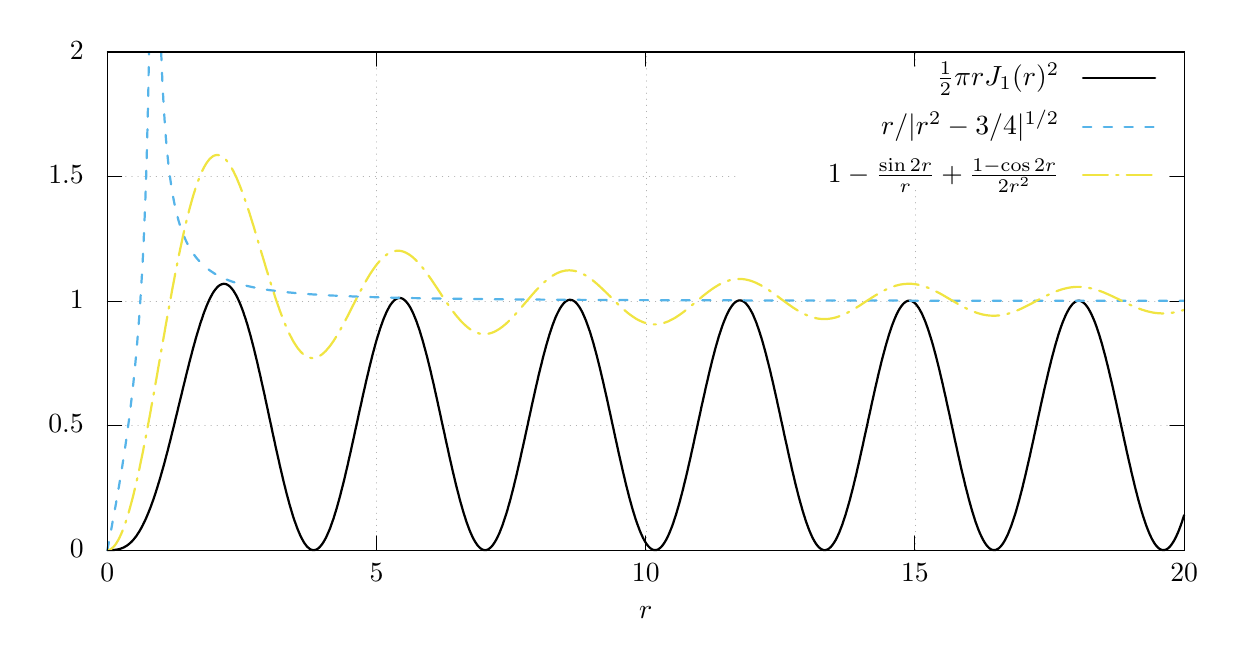
\begin{tikzpicture}[gnuplot]
	%% generated with GNUPLOT 6.0p4 (Lua 5.4; terminal rev. Jun 2020, script rev. 120)
	%% 2026/06/01 15:56:30
	\tikzset{every node/.append style={font={\normalsize}}}
	\path (0.000,0.000) rectangle (15.240,7.620);
	\gpcolor{color=gp lt color axes}
	\gpsetlinetype{gp lt axes}
	\gpsetdashtype{gp dt axes}
	\gpsetlinewidth{0.50}
	\draw[gp path] (1.012,0.985)--(14.687,0.985);
	\gpcolor{color=gp lt color border}
	\gpsetlinetype{gp lt border}
	\gpsetdashtype{gp dt solid}
	\gpsetlinewidth{1.00}
	\draw[gp path] (1.012,0.985)--(1.192,0.985);
	\draw[gp path] (14.687,0.985)--(14.507,0.985);
	\node[gp node right] at (0.828,0.985) {$0$};
	\gpcolor{color=gp lt color axes}
	\gpsetlinetype{gp lt axes}
	\gpsetdashtype{gp dt axes}
	\gpsetlinewidth{0.50}
	\draw[gp path] (1.012,2.567)--(14.687,2.567);
	\gpcolor{color=gp lt color border}
	\gpsetlinetype{gp lt border}
	\gpsetdashtype{gp dt solid}
	\gpsetlinewidth{1.00}
	\draw[gp path] (1.012,2.567)--(1.192,2.567);
	\draw[gp path] (14.687,2.567)--(14.507,2.567);
	\node[gp node right] at (0.828,2.567) {$0.5$};
	\gpcolor{color=gp lt color axes}
	\gpsetlinetype{gp lt axes}
	\gpsetdashtype{gp dt axes}
	\gpsetlinewidth{0.50}
	\draw[gp path] (1.012,4.148)--(14.687,4.148);
	\gpcolor{color=gp lt color border}
	\gpsetlinetype{gp lt border}
	\gpsetdashtype{gp dt solid}
	\gpsetlinewidth{1.00}
	\draw[gp path] (1.012,4.148)--(1.192,4.148);
	\draw[gp path] (14.687,4.148)--(14.507,4.148);
	\node[gp node right] at (0.828,4.148) {$1$};
	\gpcolor{color=gp lt color axes}
	\gpsetlinetype{gp lt axes}
	\gpsetdashtype{gp dt axes}
	\gpsetlinewidth{0.50}
	\draw[gp path] (1.012,5.730)--(8.987,5.730);
	\draw[gp path] (14.503,5.730)--(14.687,5.730);
	\gpcolor{color=gp lt color border}
	\gpsetlinetype{gp lt border}
	\gpsetdashtype{gp dt solid}
	\gpsetlinewidth{1.00}
	\draw[gp path] (1.012,5.730)--(1.192,5.730);
	\draw[gp path] (14.687,5.730)--(14.507,5.730);
	\node[gp node right] at (0.828,5.730) {$1.5$};
	\gpcolor{color=gp lt color axes}
	\gpsetlinetype{gp lt axes}
	\gpsetdashtype{gp dt axes}
	\gpsetlinewidth{0.50}
	\draw[gp path] (1.012,7.311)--(14.687,7.311);
	\gpcolor{color=gp lt color border}
	\gpsetlinetype{gp lt border}
	\gpsetdashtype{gp dt solid}
	\gpsetlinewidth{1.00}
	\draw[gp path] (1.012,7.311)--(1.192,7.311);
	\draw[gp path] (14.687,7.311)--(14.507,7.311);
	\node[gp node right] at (0.828,7.311) {$2$};
	\gpcolor{color=gp lt color axes}
	\gpsetlinetype{gp lt axes}
	\gpsetdashtype{gp dt axes}
	\gpsetlinewidth{0.50}
	\draw[gp path] (1.012,0.985)--(1.012,7.311);
	\gpcolor{color=gp lt color border}
	\gpsetlinetype{gp lt border}
	\gpsetdashtype{gp dt solid}
	\gpsetlinewidth{1.00}
	\draw[gp path] (1.012,0.985)--(1.012,1.165);
	\draw[gp path] (1.012,7.311)--(1.012,7.131);
	\node[gp node center] at (1.012,0.677) {$0$};
	\gpcolor{color=gp lt color axes}
	\gpsetlinetype{gp lt axes}
	\gpsetdashtype{gp dt axes}
	\gpsetlinewidth{0.50}
	\draw[gp path] (4.431,0.985)--(4.431,7.311);
	\gpcolor{color=gp lt color border}
	\gpsetlinetype{gp lt border}
	\gpsetdashtype{gp dt solid}
	\gpsetlinewidth{1.00}
	\draw[gp path] (4.431,0.985)--(4.431,1.165);
	\draw[gp path] (4.431,7.311)--(4.431,7.131);
	\node[gp node center] at (4.431,0.677) {$5$};
	\gpcolor{color=gp lt color axes}
	\gpsetlinetype{gp lt axes}
	\gpsetdashtype{gp dt axes}
	\gpsetlinewidth{0.50}
	\draw[gp path] (7.850,0.985)--(7.850,7.311);
	\gpcolor{color=gp lt color border}
	\gpsetlinetype{gp lt border}
	\gpsetdashtype{gp dt solid}
	\gpsetlinewidth{1.00}
	\draw[gp path] (7.850,0.985)--(7.850,1.165);
	\draw[gp path] (7.850,7.311)--(7.850,7.131);
	\node[gp node center] at (7.850,0.677) {$10$};
	\gpcolor{color=gp lt color axes}
	\gpsetlinetype{gp lt axes}
	\gpsetdashtype{gp dt axes}
	\gpsetlinewidth{0.50}
	\draw[gp path] (11.268,0.985)--(11.268,5.591);
	\draw[gp path] (11.268,7.131)--(11.268,7.311);
	\gpcolor{color=gp lt color border}
	\gpsetlinetype{gp lt border}
	\gpsetdashtype{gp dt solid}
	\gpsetlinewidth{1.00}
	\draw[gp path] (11.268,0.985)--(11.268,1.165);
	\draw[gp path] (11.268,7.311)--(11.268,7.131);
	\node[gp node center] at (11.268,0.677) {$15$};
	\gpcolor{color=gp lt color axes}
	\gpsetlinetype{gp lt axes}
	\gpsetdashtype{gp dt axes}
	\gpsetlinewidth{0.50}
	\draw[gp path] (14.687,0.985)--(14.687,7.311);
	\gpcolor{color=gp lt color border}
	\gpsetlinetype{gp lt border}
	\gpsetdashtype{gp dt solid}
	\gpsetlinewidth{1.00}
	\draw[gp path] (14.687,0.985)--(14.687,1.165);
	\draw[gp path] (14.687,7.311)--(14.687,7.131);
	\node[gp node center] at (14.687,0.677) {$20$};
	\draw[gp path] (1.012,7.311)--(1.012,0.985)--(14.687,0.985)--(14.687,7.311)--cycle;
	\node[gp node right] at (13.219,6.977) {$\frac{1}{2} \pi r \BesselJ{1}(r)^2$};
	\gpcolor{rgb color={0.000,0.000,0.000}}
	\gpsetdashtype{gp dt 1}
	\gpsetlinewidth{2.00}
	\draw[gp path] (13.403,6.977)--(14.319,6.977);
	\draw[gp path] (1.012,0.985)--(1.026,0.985)--(1.039,0.985)--(1.053,0.985)--(1.067,0.986)%
	--(1.080,0.986)--(1.094,0.987)--(1.108,0.988)--(1.122,0.990)--(1.135,0.992)--(1.149,0.995)%
	--(1.163,0.998)--(1.176,1.002)--(1.190,1.007)--(1.204,1.012)--(1.217,1.018)--(1.231,1.025)%
	--(1.245,1.033)--(1.258,1.041)--(1.272,1.051)--(1.286,1.062)--(1.299,1.073)--(1.313,1.086)%
	--(1.327,1.100)--(1.341,1.115)--(1.354,1.131)--(1.368,1.149)--(1.382,1.167)--(1.395,1.187)%
	--(1.409,1.208)--(1.423,1.231)--(1.436,1.254)--(1.450,1.279)--(1.464,1.306)--(1.477,1.333)%
	--(1.491,1.362)--(1.505,1.393)--(1.518,1.424)--(1.532,1.457)--(1.546,1.492)--(1.560,1.527)%
	--(1.573,1.564)--(1.587,1.602)--(1.601,1.641)--(1.614,1.682)--(1.628,1.724)--(1.642,1.767)%
	--(1.655,1.811)--(1.669,1.856)--(1.683,1.902)--(1.696,1.949)--(1.710,1.998)--(1.724,2.047)%
	--(1.738,2.097)--(1.751,2.148)--(1.765,2.200)--(1.779,2.252)--(1.792,2.305)--(1.806,2.359)%
	--(1.820,2.414)--(1.833,2.469)--(1.847,2.524)--(1.861,2.580)--(1.874,2.636)--(1.888,2.692)%
	--(1.902,2.749)--(1.915,2.805)--(1.929,2.862)--(1.943,2.919)--(1.957,2.975)--(1.970,3.032)%
	--(1.984,3.088)--(1.998,3.144)--(2.011,3.199)--(2.025,3.255)--(2.039,3.309)--(2.052,3.363)%
	--(2.066,3.416)--(2.080,3.469)--(2.093,3.520)--(2.107,3.571)--(2.121,3.621)--(2.134,3.669)%
	--(2.148,3.717)--(2.162,3.763)--(2.176,3.808)--(2.189,3.852)--(2.203,3.894)--(2.217,3.935)%
	--(2.230,3.975)--(2.244,4.013)--(2.258,4.049)--(2.271,4.083)--(2.285,4.116)--(2.299,4.147)%
	--(2.312,4.176)--(2.326,4.203)--(2.340,4.228)--(2.353,4.252)--(2.367,4.273)--(2.381,4.292)%
	--(2.395,4.309)--(2.408,4.324)--(2.422,4.337)--(2.436,4.347)--(2.449,4.355)--(2.463,4.361)%
	--(2.477,4.365)--(2.490,4.367)--(2.504,4.366)--(2.518,4.363)--(2.531,4.358)--(2.545,4.350)%
	--(2.559,4.340)--(2.573,4.328)--(2.586,4.314)--(2.600,4.297)--(2.614,4.278)--(2.627,4.257)%
	--(2.641,4.234)--(2.655,4.208)--(2.668,4.181)--(2.682,4.151)--(2.696,4.119)--(2.709,4.086)%
	--(2.723,4.050)--(2.737,4.012)--(2.750,3.972)--(2.764,3.931)--(2.778,3.888)--(2.792,3.843)%
	--(2.805,3.796)--(2.819,3.748)--(2.833,3.698)--(2.846,3.647)--(2.860,3.594)--(2.874,3.540)%
	--(2.887,3.485)--(2.901,3.428)--(2.915,3.371)--(2.928,3.312)--(2.942,3.252)--(2.956,3.192)%
	--(2.969,3.131)--(2.983,3.069)--(2.997,3.007)--(3.011,2.944)--(3.024,2.880)--(3.038,2.817)%
	--(3.052,2.753)--(3.065,2.689)--(3.079,2.625)--(3.093,2.561)--(3.106,2.497)--(3.120,2.433)%
	--(3.134,2.370)--(3.147,2.307)--(3.161,2.245)--(3.175,2.183)--(3.189,2.122)--(3.202,2.061)%
	--(3.216,2.002)--(3.230,1.943)--(3.243,1.886)--(3.257,1.829)--(3.271,1.774)--(3.284,1.720)%
	--(3.298,1.668)--(3.312,1.617)--(3.325,1.567)--(3.339,1.520)--(3.353,1.473)--(3.366,1.429)%
	--(3.380,1.386)--(3.394,1.345)--(3.408,1.307)--(3.421,1.270)--(3.435,1.235)--(3.449,1.202)%
	--(3.462,1.171)--(3.476,1.143)--(3.490,1.117)--(3.503,1.093)--(3.517,1.071)--(3.531,1.052)%
	--(3.544,1.035)--(3.558,1.021)--(3.572,1.009)--(3.585,0.999)--(3.599,0.992)--(3.613,0.987)%
	--(3.627,0.985)--(3.640,0.985)--(3.654,0.988)--(3.668,0.993)--(3.681,1.001)--(3.695,1.011)%
	--(3.709,1.024)--(3.722,1.039)--(3.736,1.056)--(3.750,1.076)--(3.763,1.098)--(3.777,1.122)%
	--(3.791,1.149)--(3.804,1.178)--(3.818,1.209)--(3.832,1.242)--(3.846,1.277)--(3.859,1.315)%
	--(3.873,1.354)--(3.887,1.395)--(3.900,1.438)--(3.914,1.483)--(3.928,1.529)--(3.941,1.577)%
	--(3.955,1.627)--(3.969,1.678)--(3.982,1.731)--(3.996,1.785)--(4.010,1.840)--(4.024,1.896)%
	--(4.037,1.954)--(4.051,2.012)--(4.065,2.071)--(4.078,2.132)--(4.092,2.192)--(4.106,2.254)%
	--(4.119,2.316)--(4.133,2.378)--(4.147,2.441)--(4.160,2.504)--(4.174,2.567)--(4.188,2.630)%
	--(4.201,2.693)--(4.215,2.756)--(4.229,2.818)--(4.243,2.881)--(4.256,2.943)--(4.270,3.004)%
	--(4.284,3.064)--(4.297,3.124)--(4.311,3.183)--(4.325,3.241)--(4.338,3.298)--(4.352,3.354)%
	--(4.366,3.409)--(4.379,3.463)--(4.393,3.515)--(4.407,3.566)--(4.420,3.615)--(4.434,3.663)%
	--(4.448,3.708)--(4.462,3.753)--(4.475,3.795)--(4.489,3.835)--(4.503,3.874)--(4.516,3.911)%
	--(4.530,3.945)--(4.544,3.977)--(4.557,4.008)--(4.571,4.036)--(4.585,4.061)--(4.598,4.085)%
	--(4.612,4.106)--(4.626,4.125)--(4.640,4.141)--(4.653,4.155)--(4.667,4.166)--(4.681,4.175)%
	--(4.694,4.182)--(4.708,4.186)--(4.722,4.187)--(4.735,4.186)--(4.749,4.183)--(4.763,4.177)%
	--(4.776,4.168)--(4.790,4.157)--(4.804,4.144)--(4.817,4.128)--(4.831,4.110)--(4.845,4.089)%
	--(4.859,4.066)--(4.872,4.041)--(4.886,4.013)--(4.900,3.983)--(4.913,3.951)--(4.927,3.917)%
	--(4.941,3.881)--(4.954,3.843)--(4.968,3.802)--(4.982,3.760)--(4.995,3.716)--(5.009,3.671)%
	--(5.023,3.623)--(5.036,3.574)--(5.050,3.523)--(5.064,3.471)--(5.078,3.418)--(5.091,3.363)%
	--(5.105,3.307)--(5.119,3.250)--(5.132,3.192)--(5.146,3.133)--(5.160,3.073)--(5.173,3.012)%
	--(5.187,2.950)--(5.201,2.888)--(5.214,2.826)--(5.228,2.763)--(5.242,2.700)--(5.255,2.636)%
	--(5.269,2.573)--(5.283,2.510)--(5.297,2.446)--(5.310,2.383)--(5.324,2.321)--(5.338,2.258)%
	--(5.351,2.196)--(5.365,2.135)--(5.379,2.075)--(5.392,2.015)--(5.406,1.956)--(5.420,1.898)%
	--(5.433,1.842)--(5.447,1.786)--(5.461,1.732)--(5.475,1.679)--(5.488,1.627)--(5.502,1.577)%
	--(5.516,1.529)--(5.529,1.482)--(5.543,1.437)--(5.557,1.394)--(5.570,1.352)--(5.584,1.313)%
	--(5.598,1.275)--(5.611,1.240)--(5.625,1.207)--(5.639,1.175)--(5.652,1.147)--(5.666,1.120)%
	--(5.680,1.096)--(5.694,1.074)--(5.707,1.054)--(5.721,1.037)--(5.735,1.022)--(5.748,1.010)%
	--(5.762,1.000)--(5.776,0.992)--(5.789,0.988)--(5.803,0.985)--(5.817,0.985)--(5.830,0.988)%
	--(5.844,0.993)--(5.858,1.001)--(5.871,1.011)--(5.885,1.024)--(5.899,1.039)--(5.913,1.057)%
	--(5.926,1.077)--(5.940,1.099)--(5.954,1.124)--(5.967,1.151)--(5.981,1.180)--(5.995,1.211)%
	--(6.008,1.245)--(6.022,1.280)--(6.036,1.318)--(6.049,1.358)--(6.063,1.400)--(6.077,1.443)%
	--(6.091,1.488)--(6.104,1.536)--(6.118,1.584)--(6.132,1.634)--(6.145,1.686)--(6.159,1.739)%
	--(6.173,1.794)--(6.186,1.850)--(6.200,1.906)--(6.214,1.964)--(6.227,2.023)--(6.241,2.083)%
	--(6.255,2.143)--(6.268,2.205)--(6.282,2.267)--(6.296,2.329)--(6.310,2.392)--(6.323,2.454)%
	--(6.337,2.518)--(6.351,2.581)--(6.364,2.644)--(6.378,2.707)--(6.392,2.770)--(6.405,2.833)%
	--(6.419,2.895)--(6.433,2.957)--(6.446,3.018)--(6.460,3.078)--(6.474,3.138)--(6.487,3.197)%
	--(6.501,3.254)--(6.515,3.311)--(6.529,3.366)--(6.542,3.421)--(6.556,3.474)--(6.570,3.525)%
	--(6.583,3.575)--(6.597,3.623)--(6.611,3.670)--(6.624,3.715)--(6.638,3.758)--(6.652,3.800)%
	--(6.665,3.839)--(6.679,3.876)--(6.693,3.912)--(6.706,3.945)--(6.720,3.976)--(6.734,4.004)%
	--(6.748,4.031)--(6.761,4.055)--(6.775,4.077)--(6.789,4.096)--(6.802,4.113)--(6.816,4.128)%
	--(6.830,4.140)--(6.843,4.150)--(6.857,4.157)--(6.871,4.162)--(6.884,4.164)--(6.898,4.163)%
	--(6.912,4.160)--(6.926,4.155)--(6.939,4.147)--(6.953,4.137)--(6.967,4.124)--(6.980,4.108)%
	--(6.994,4.090)--(7.008,4.070)--(7.021,4.048)--(7.035,4.023)--(7.049,3.995)--(7.062,3.966)%
	--(7.076,3.934)--(7.090,3.900)--(7.103,3.864)--(7.117,3.826)--(7.131,3.786)--(7.145,3.745)%
	--(7.158,3.701)--(7.172,3.655)--(7.186,3.608)--(7.199,3.559)--(7.213,3.508)--(7.227,3.456)%
	--(7.240,3.403)--(7.254,3.348)--(7.268,3.292)--(7.281,3.235)--(7.295,3.177)--(7.309,3.118)%
	--(7.322,3.058)--(7.336,2.998)--(7.350,2.936)--(7.364,2.874)--(7.377,2.812)--(7.391,2.749)%
	--(7.405,2.686)--(7.418,2.623)--(7.432,2.559)--(7.446,2.496)--(7.459,2.433)--(7.473,2.370)%
	--(7.487,2.307)--(7.500,2.245)--(7.514,2.183)--(7.528,2.122)--(7.542,2.062)--(7.555,2.002)%
	--(7.569,1.944)--(7.583,1.886)--(7.596,1.829)--(7.610,1.774)--(7.624,1.720)--(7.637,1.667)%
	--(7.651,1.616)--(7.665,1.566)--(7.678,1.518)--(7.692,1.472)--(7.706,1.427)--(7.719,1.384)%
	--(7.733,1.343)--(7.747,1.304)--(7.761,1.267)--(7.774,1.232)--(7.788,1.199)--(7.802,1.168)%
	--(7.815,1.140)--(7.829,1.114)--(7.843,1.090)--(7.856,1.068)--(7.870,1.049)--(7.884,1.033)%
	--(7.897,1.019)--(7.911,1.007)--(7.925,0.998)--(7.938,0.991)--(7.952,0.987)--(7.966,0.985)%
	--(7.980,0.986)--(7.993,0.989)--(8.007,0.995)--(8.021,1.004)--(8.034,1.014)--(8.048,1.028)%
	--(8.062,1.044)--(8.075,1.062)--(8.089,1.083)--(8.103,1.106)--(8.116,1.131)--(8.130,1.159)%
	--(8.144,1.189)--(8.157,1.221)--(8.171,1.255)--(8.185,1.291)--(8.199,1.330)--(8.212,1.370)%
	--(8.226,1.412)--(8.240,1.457)--(8.253,1.503)--(8.267,1.550)--(8.281,1.599)--(8.294,1.650)%
	--(8.308,1.702)--(8.322,1.756)--(8.335,1.811)--(8.349,1.867)--(8.363,1.924)--(8.377,1.983)%
	--(8.390,2.042)--(8.404,2.102)--(8.418,2.163)--(8.431,2.224)--(8.445,2.286)--(8.459,2.349)%
	--(8.472,2.412)--(8.486,2.475)--(8.500,2.538)--(8.513,2.601)--(8.527,2.665)--(8.541,2.728)%
	--(8.554,2.791)--(8.568,2.853)--(8.582,2.915)--(8.596,2.977)--(8.609,3.038)--(8.623,3.098)%
	--(8.637,3.157)--(8.650,3.215)--(8.664,3.273)--(8.678,3.329)--(8.691,3.384)--(8.705,3.437)%
	--(8.719,3.490)--(8.732,3.541)--(8.746,3.590)--(8.760,3.638)--(8.773,3.684)--(8.787,3.728)%
	--(8.801,3.770)--(8.815,3.811)--(8.828,3.849)--(8.842,3.886)--(8.856,3.920)--(8.869,3.952)%
	--(8.883,3.982)--(8.897,4.010)--(8.910,4.035)--(8.924,4.058)--(8.938,4.079)--(8.951,4.097)%
	--(8.965,4.113)--(8.979,4.127)--(8.993,4.138)--(9.006,4.146)--(9.020,4.152)--(9.034,4.156)%
	--(9.047,4.157)--(9.061,4.155)--(9.075,4.151)--(9.088,4.144)--(9.102,4.135)--(9.116,4.123)%
	--(9.129,4.109)--(9.143,4.092)--(9.157,4.073)--(9.170,4.052)--(9.184,4.028)--(9.198,4.002)%
	--(9.212,3.974)--(9.225,3.943)--(9.239,3.910)--(9.253,3.875)--(9.266,3.838)--(9.280,3.799)%
	--(9.294,3.758)--(9.307,3.715)--(9.321,3.671)--(9.335,3.624)--(9.348,3.576)--(9.362,3.526)%
	--(9.376,3.475)--(9.389,3.422)--(9.403,3.368)--(9.417,3.313)--(9.431,3.256)--(9.444,3.199)%
	--(9.458,3.140)--(9.472,3.080)--(9.485,3.020)--(9.499,2.959)--(9.513,2.897)--(9.526,2.835)%
	--(9.540,2.772)--(9.554,2.709)--(9.567,2.646)--(9.581,2.583)--(9.595,2.520)--(9.608,2.456)%
	--(9.622,2.393)--(9.636,2.331)--(9.650,2.268)--(9.663,2.206)--(9.677,2.145)--(9.691,2.084)%
	--(9.704,2.024)--(9.718,1.965)--(9.732,1.907)--(9.745,1.850)--(9.759,1.794)--(9.773,1.740)%
	--(9.786,1.687)--(9.800,1.635)--(9.814,1.584)--(9.828,1.536)--(9.841,1.488)--(9.855,1.443)%
	--(9.869,1.399)--(9.882,1.358)--(9.896,1.318)--(9.910,1.280)--(9.923,1.244)--(9.937,1.211)%
	--(9.951,1.179)--(9.964,1.150)--(9.978,1.123)--(9.992,1.098)--(10.005,1.076)--(10.019,1.056)%
	--(10.033,1.038)--(10.047,1.023)--(10.060,1.011)--(10.074,1.001)--(10.088,0.993)--(10.101,0.988)%
	--(10.115,0.985)--(10.129,0.985)--(10.142,0.988)--(10.156,0.993)--(10.170,1.000)--(10.183,1.010)%
	--(10.197,1.023)--(10.211,1.038)--(10.224,1.055)--(10.238,1.075)--(10.252,1.097)--(10.266,1.122)%
	--(10.279,1.149)--(10.293,1.178)--(10.307,1.209)--(10.320,1.243)--(10.334,1.279)--(10.348,1.316)%
	--(10.361,1.356)--(10.375,1.398)--(10.389,1.441)--(10.402,1.487)--(10.416,1.534)--(10.430,1.583)%
	--(10.444,1.633)--(10.457,1.685)--(10.471,1.738)--(10.485,1.792)--(10.498,1.848)--(10.512,1.905)%
	--(10.526,1.963)--(10.539,2.022)--(10.553,2.082)--(10.567,2.143)--(10.580,2.204)--(10.594,2.266)%
	--(10.608,2.328)--(10.621,2.391)--(10.635,2.454)--(10.649,2.517)--(10.663,2.580)--(10.676,2.644)%
	--(10.690,2.707)--(10.704,2.770)--(10.717,2.832)--(10.731,2.895)--(10.745,2.956)--(10.758,3.017)%
	--(10.772,3.078)--(10.786,3.137)--(10.799,3.196)--(10.813,3.254)--(10.827,3.310)--(10.840,3.365)%
	--(10.854,3.420)--(10.868,3.472)--(10.882,3.524)--(10.895,3.573)--(10.909,3.622)--(10.923,3.668)%
	--(10.936,3.713)--(10.950,3.756)--(10.964,3.797)--(10.977,3.836)--(10.991,3.873)--(11.005,3.908)%
	--(11.018,3.940)--(11.032,3.971)--(11.046,3.999)--(11.059,4.025)--(11.073,4.049)--(11.087,4.071)%
	--(11.101,4.090)--(11.114,4.106)--(11.128,4.120)--(11.142,4.132)--(11.155,4.141)--(11.169,4.148)%
	--(11.183,4.152)--(11.196,4.153)--(11.210,4.152)--(11.224,4.149)--(11.237,4.143)--(11.251,4.134)%
	--(11.265,4.123)--(11.279,4.110)--(11.292,4.094)--(11.306,4.075)--(11.320,4.055)--(11.333,4.031)%
	--(11.347,4.006)--(11.361,3.978)--(11.374,3.948)--(11.388,3.916)--(11.402,3.881)--(11.415,3.845)%
	--(11.429,3.806)--(11.443,3.766)--(11.456,3.723)--(11.470,3.679)--(11.484,3.633)--(11.498,3.585)%
	--(11.511,3.536)--(11.525,3.485)--(11.539,3.432)--(11.552,3.379)--(11.566,3.324)--(11.580,3.267)%
	--(11.593,3.210)--(11.607,3.152)--(11.621,3.092)--(11.634,3.032)--(11.648,2.971)--(11.662,2.910)%
	--(11.675,2.847)--(11.689,2.785)--(11.703,2.722)--(11.717,2.659)--(11.730,2.596)--(11.744,2.532)%
	--(11.758,2.469)--(11.771,2.406)--(11.785,2.343)--(11.799,2.281)--(11.812,2.218)--(11.826,2.157)%
	--(11.840,2.096)--(11.853,2.036)--(11.867,1.977)--(11.881,1.919)--(11.895,1.862)--(11.908,1.805)%
	--(11.922,1.751)--(11.936,1.697)--(11.949,1.645)--(11.963,1.594)--(11.977,1.545)--(11.990,1.498)%
	--(12.004,1.452)--(12.018,1.408)--(12.031,1.366)--(12.045,1.325)--(12.059,1.287)--(12.072,1.251)%
	--(12.086,1.217)--(12.100,1.185)--(12.114,1.155)--(12.127,1.128)--(12.141,1.103)--(12.155,1.080)%
	--(12.168,1.060)--(12.182,1.042)--(12.196,1.026)--(12.209,1.013)--(12.223,1.002)--(12.237,0.994)%
	--(12.250,0.989)--(12.264,0.986)--(12.278,0.985)--(12.291,0.987)--(12.305,0.992)--(12.319,0.999)%
	--(12.333,1.008)--(12.346,1.020)--(12.360,1.035)--(12.374,1.052)--(12.387,1.071)--(12.401,1.093)%
	--(12.415,1.117)--(12.428,1.144)--(12.442,1.172)--(12.456,1.203)--(12.469,1.237)--(12.483,1.272)%
	--(12.497,1.309)--(12.510,1.349)--(12.524,1.390)--(12.538,1.433)--(12.552,1.478)--(12.565,1.525)%
	--(12.579,1.574)--(12.593,1.624)--(12.606,1.675)--(12.620,1.728)--(12.634,1.782)--(12.647,1.838)%
	--(12.661,1.895)--(12.675,1.953)--(12.688,2.011)--(12.702,2.071)--(12.716,2.132)--(12.730,2.193)%
	--(12.743,2.255)--(12.757,2.317)--(12.771,2.380)--(12.784,2.443)--(12.798,2.506)--(12.812,2.569)%
	--(12.825,2.632)--(12.839,2.696)--(12.853,2.759)--(12.866,2.821)--(12.880,2.884)--(12.894,2.945)%
	--(12.907,3.007)--(12.921,3.067)--(12.935,3.127)--(12.949,3.185)--(12.962,3.243)--(12.976,3.300)%
	--(12.990,3.356)--(13.003,3.410)--(13.017,3.463)--(13.031,3.514)--(13.044,3.564)--(13.058,3.613)%
	--(13.072,3.659)--(13.085,3.704)--(13.099,3.748)--(13.113,3.789)--(13.126,3.828)--(13.140,3.866)%
	--(13.154,3.901)--(13.168,3.934)--(13.181,3.965)--(13.195,3.994)--(13.209,4.020)--(13.222,4.044)%
	--(13.236,4.066)--(13.250,4.085)--(13.263,4.102)--(13.277,4.117)--(13.291,4.129)--(13.304,4.138)%
	--(13.318,4.145)--(13.332,4.150)--(13.346,4.152)--(13.359,4.151)--(13.373,4.148)--(13.387,4.142)%
	--(13.400,4.134)--(13.414,4.123)--(13.428,4.110)--(13.441,4.095)--(13.455,4.076)--(13.469,4.056)%
	--(13.482,4.033)--(13.496,4.008)--(13.510,3.980)--(13.523,3.951)--(13.537,3.919)--(13.551,3.885)%
	--(13.565,3.848)--(13.578,3.810)--(13.592,3.770)--(13.606,3.728)--(13.619,3.684)--(13.633,3.638)%
	--(13.647,3.590)--(13.660,3.541)--(13.674,3.490)--(13.688,3.438)--(13.701,3.384)--(13.715,3.330)%
	--(13.729,3.273)--(13.742,3.216)--(13.756,3.158)--(13.770,3.099)--(13.784,3.039)--(13.797,2.978)%
	--(13.811,2.916)--(13.825,2.854)--(13.838,2.792)--(13.852,2.729)--(13.866,2.666)--(13.879,2.602)%
	--(13.893,2.539)--(13.907,2.476)--(13.920,2.413)--(13.934,2.350)--(13.948,2.287)--(13.961,2.225)%
	--(13.975,2.164)--(13.989,2.103)--(14.003,2.043)--(14.016,1.983)--(14.030,1.925)--(14.044,1.868)%
	--(14.057,1.811)--(14.071,1.756)--(14.085,1.703)--(14.098,1.650)--(14.112,1.600)--(14.126,1.550)%
	--(14.139,1.503)--(14.153,1.457)--(14.167,1.412)--(14.181,1.370)--(14.194,1.330)--(14.208,1.291)%
	--(14.222,1.255)--(14.235,1.221)--(14.249,1.188)--(14.263,1.158)--(14.276,1.131)--(14.290,1.105)%
	--(14.304,1.082)--(14.317,1.062)--(14.331,1.043)--(14.345,1.028)--(14.358,1.014)--(14.372,1.003)%
	--(14.386,0.995)--(14.400,0.989)--(14.413,0.986)--(14.427,0.985)--(14.441,0.987)--(14.454,0.991)%
	--(14.468,0.998)--(14.482,1.007)--(14.495,1.019)--(14.509,1.033)--(14.523,1.050)--(14.536,1.069)%
	--(14.550,1.091)--(14.564,1.115)--(14.577,1.141)--(14.591,1.169)--(14.605,1.200)--(14.619,1.233)%
	--(14.632,1.268)--(14.646,1.305)--(14.660,1.345)--(14.673,1.386)--(14.687,1.429);
	\gpcolor{color=gp lt color border}
	\node[gp node right] at (13.219,6.669) { };
	\gpcolor{color=gpbgfillcolor}
	\gpsetlinetype{gp lt plot 4}
	\gpsetdashtype{gp dt solid}
	\gpsetlinewidth{1.00}
	\draw[gp path] (13.403,6.669)--(14.319,6.669);
	\gpcolor{color=gp lt color border}
	\node[gp node right] at (13.219,6.361) {$r/\abs{r^2 - 3/4}^{1/2}$};
	\gpcolor{rgb color={0.337,0.706,0.914}}
	\gpsetlinetype{gp lt border}
	\gpsetdashtype{gp dt 3}
	\gpsetlinewidth{2.00}
	\draw[gp path] (13.403,6.361)--(14.319,6.361);
	\draw[gp path] (1.012,0.985)--(1.026,1.058)--(1.039,1.131)--(1.053,1.205)--(1.067,1.279)%
	--(1.080,1.353)--(1.094,1.428)--(1.108,1.504)--(1.122,1.580)--(1.135,1.658)--(1.149,1.737)%
	--(1.163,1.817)--(1.176,1.898)--(1.190,1.982)--(1.204,2.067)--(1.217,2.154)--(1.231,2.244)%
	--(1.245,2.337)--(1.258,2.432)--(1.272,2.531)--(1.286,2.634)--(1.299,2.741)--(1.313,2.853)%
	--(1.327,2.971)--(1.341,3.094)--(1.354,3.225)--(1.368,3.364)--(1.382,3.512)--(1.395,3.671)%
	--(1.409,3.843)--(1.423,4.030)--(1.436,4.235)--(1.450,4.462)--(1.464,4.717)--(1.477,5.006)%
	--(1.491,5.340)--(1.505,5.733)--(1.518,6.207)--(1.532,6.800)--(1.541,7.311);
	\draw[gp path] (1.695,7.311)--(1.696,7.292)--(1.710,6.956)--(1.724,6.685)--(1.738,6.459)%
	--(1.751,6.269)--(1.765,6.107)--(1.779,5.966)--(1.792,5.842)--(1.806,5.733)--(1.820,5.636)%
	--(1.833,5.549)--(1.847,5.471)--(1.861,5.400)--(1.874,5.336)--(1.888,5.277)--(1.902,5.223)%
	--(1.915,5.173)--(1.929,5.127)--(1.943,5.084)--(1.957,5.045)--(1.970,5.008)--(1.984,4.974)%
	--(1.998,4.942)--(2.011,4.912)--(2.025,4.883)--(2.039,4.857)--(2.052,4.832)--(2.066,4.808)%
	--(2.080,4.786)--(2.093,4.765)--(2.107,4.745)--(2.121,4.726)--(2.134,4.708)--(2.148,4.691)%
	--(2.162,4.675)--(2.176,4.659)--(2.189,4.645)--(2.203,4.631)--(2.217,4.617)--(2.230,4.604)%
	--(2.244,4.592)--(2.258,4.580)--(2.271,4.569)--(2.285,4.558)--(2.299,4.548)--(2.312,4.538)%
	--(2.326,4.528)--(2.340,4.519)--(2.353,4.510)--(2.367,4.501)--(2.381,4.493)--(2.395,4.485)%
	--(2.408,4.478)--(2.422,4.470)--(2.436,4.463)--(2.449,4.456)--(2.463,4.450)--(2.477,4.443)%
	--(2.490,4.437)--(2.504,4.431)--(2.518,4.425)--(2.531,4.420)--(2.545,4.414)--(2.559,4.409)%
	--(2.573,4.404)--(2.586,4.399)--(2.600,4.394)--(2.614,4.389)--(2.627,4.385)--(2.641,4.380)%
	--(2.655,4.376)--(2.668,4.372)--(2.682,4.368)--(2.696,4.364)--(2.709,4.360)--(2.723,4.356)%
	--(2.737,4.353)--(2.750,4.349)--(2.764,4.346)--(2.778,4.342)--(2.792,4.339)--(2.805,4.336)%
	--(2.819,4.333)--(2.833,4.330)--(2.846,4.327)--(2.860,4.324)--(2.874,4.321)--(2.887,4.319)%
	--(2.901,4.316)--(2.915,4.313)--(2.928,4.311)--(2.942,4.308)--(2.956,4.306)--(2.969,4.303)%
	--(2.983,4.301)--(2.997,4.299)--(3.011,4.297)--(3.024,4.295)--(3.038,4.292)--(3.052,4.290)%
	--(3.065,4.288)--(3.079,4.286)--(3.093,4.284)--(3.106,4.283)--(3.120,4.281)--(3.134,4.279)%
	--(3.147,4.277)--(3.161,4.275)--(3.175,4.274)--(3.189,4.272)--(3.202,4.270)--(3.216,4.269)%
	--(3.230,4.267)--(3.243,4.266)--(3.257,4.264)--(3.271,4.263)--(3.284,4.261)--(3.298,4.260)%
	--(3.312,4.258)--(3.325,4.257)--(3.339,4.256)--(3.353,4.254)--(3.366,4.253)--(3.380,4.252)%
	--(3.394,4.251)--(3.408,4.249)--(3.421,4.248)--(3.435,4.247)--(3.449,4.246)--(3.462,4.245)%
	--(3.476,4.243)--(3.490,4.242)--(3.503,4.241)--(3.517,4.240)--(3.531,4.239)--(3.544,4.238)%
	--(3.558,4.237)--(3.572,4.236)--(3.585,4.235)--(3.599,4.234)--(3.613,4.233)--(3.627,4.232)%
	--(3.640,4.231)--(3.654,4.231)--(3.668,4.230)--(3.681,4.229)--(3.695,4.228)--(3.709,4.227)%
	--(3.722,4.226)--(3.736,4.225)--(3.750,4.225)--(3.763,4.224)--(3.777,4.223)--(3.791,4.222)%
	--(3.804,4.222)--(3.818,4.221)--(3.832,4.220)--(3.846,4.219)--(3.859,4.219)--(3.873,4.218)%
	--(3.887,4.217)--(3.900,4.217)--(3.914,4.216)--(3.928,4.215)--(3.941,4.215)--(3.955,4.214)%
	--(3.969,4.213)--(3.982,4.213)--(3.996,4.212)--(4.010,4.212)--(4.024,4.211)--(4.037,4.210)%
	--(4.051,4.210)--(4.065,4.209)--(4.078,4.209)--(4.092,4.208)--(4.106,4.208)--(4.119,4.207)%
	--(4.133,4.207)--(4.147,4.206)--(4.160,4.205)--(4.174,4.205)--(4.188,4.204)--(4.201,4.204)%
	--(4.215,4.203)--(4.229,4.203)--(4.243,4.203)--(4.256,4.202)--(4.270,4.202)--(4.284,4.201)%
	--(4.297,4.201)--(4.311,4.200)--(4.325,4.200)--(4.338,4.199)--(4.352,4.199)--(4.366,4.198)%
	--(4.379,4.198)--(4.393,4.198)--(4.407,4.197)--(4.420,4.197)--(4.434,4.196)--(4.448,4.196)%
	--(4.462,4.196)--(4.475,4.195)--(4.489,4.195)--(4.503,4.195)--(4.516,4.194)--(4.530,4.194)%
	--(4.544,4.193)--(4.557,4.193)--(4.571,4.193)--(4.585,4.192)--(4.598,4.192)--(4.612,4.192)%
	--(4.626,4.191)--(4.640,4.191)--(4.653,4.191)--(4.667,4.190)--(4.681,4.190)--(4.694,4.190)%
	--(4.708,4.189)--(4.722,4.189)--(4.735,4.189)--(4.749,4.188)--(4.763,4.188)--(4.776,4.188)%
	--(4.790,4.188)--(4.804,4.187)--(4.817,4.187)--(4.831,4.187)--(4.845,4.186)--(4.859,4.186)%
	--(4.872,4.186)--(4.886,4.186)--(4.900,4.185)--(4.913,4.185)--(4.927,4.185)--(4.941,4.185)%
	--(4.954,4.184)--(4.968,4.184)--(4.982,4.184)--(4.995,4.184)--(5.009,4.183)--(5.023,4.183)%
	--(5.036,4.183)--(5.050,4.183)--(5.064,4.182)--(5.078,4.182)--(5.091,4.182)--(5.105,4.182)%
	--(5.119,4.181)--(5.132,4.181)--(5.146,4.181)--(5.160,4.181)--(5.173,4.181)--(5.187,4.180)%
	--(5.201,4.180)--(5.214,4.180)--(5.228,4.180)--(5.242,4.179)--(5.255,4.179)--(5.269,4.179)%
	--(5.283,4.179)--(5.297,4.179)--(5.310,4.178)--(5.324,4.178)--(5.338,4.178)--(5.351,4.178)%
	--(5.365,4.178)--(5.379,4.177)--(5.392,4.177)--(5.406,4.177)--(5.420,4.177)--(5.433,4.177)%
	--(5.447,4.177)--(5.461,4.176)--(5.475,4.176)--(5.488,4.176)--(5.502,4.176)--(5.516,4.176)%
	--(5.529,4.176)--(5.543,4.175)--(5.557,4.175)--(5.570,4.175)--(5.584,4.175)--(5.598,4.175)%
	--(5.611,4.175)--(5.625,4.174)--(5.639,4.174)--(5.652,4.174)--(5.666,4.174)--(5.680,4.174)%
	--(5.694,4.174)--(5.707,4.173)--(5.721,4.173)--(5.735,4.173)--(5.748,4.173)--(5.762,4.173)%
	--(5.776,4.173)--(5.789,4.173)--(5.803,4.172)--(5.817,4.172)--(5.830,4.172)--(5.844,4.172)%
	--(5.858,4.172)--(5.871,4.172)--(5.885,4.172)--(5.899,4.171)--(5.913,4.171)--(5.926,4.171)%
	--(5.940,4.171)--(5.954,4.171)--(5.967,4.171)--(5.981,4.171)--(5.995,4.171)--(6.008,4.170)%
	--(6.022,4.170)--(6.036,4.170)--(6.049,4.170)--(6.063,4.170)--(6.077,4.170)--(6.091,4.170)%
	--(6.104,4.170)--(6.118,4.169)--(6.132,4.169)--(6.145,4.169)--(6.159,4.169)--(6.173,4.169)%
	--(6.186,4.169)--(6.200,4.169)--(6.214,4.169)--(6.227,4.169)--(6.241,4.168)--(6.255,4.168)%
	--(6.268,4.168)--(6.282,4.168)--(6.296,4.168)--(6.310,4.168)--(6.323,4.168)--(6.337,4.168)%
	--(6.351,4.168)--(6.364,4.168)--(6.378,4.167)--(6.392,4.167)--(6.405,4.167)--(6.419,4.167)%
	--(6.433,4.167)--(6.446,4.167)--(6.460,4.167)--(6.474,4.167)--(6.487,4.167)--(6.501,4.167)%
	--(6.515,4.166)--(6.529,4.166)--(6.542,4.166)--(6.556,4.166)--(6.570,4.166)--(6.583,4.166)%
	--(6.597,4.166)--(6.611,4.166)--(6.624,4.166)--(6.638,4.166)--(6.652,4.166)--(6.665,4.165)%
	--(6.679,4.165)--(6.693,4.165)--(6.706,4.165)--(6.720,4.165)--(6.734,4.165)--(6.748,4.165)%
	--(6.761,4.165)--(6.775,4.165)--(6.789,4.165)--(6.802,4.165)--(6.816,4.165)--(6.830,4.165)%
	--(6.843,4.164)--(6.857,4.164)--(6.871,4.164)--(6.884,4.164)--(6.898,4.164)--(6.912,4.164)%
	--(6.926,4.164)--(6.939,4.164)--(6.953,4.164)--(6.967,4.164)--(6.980,4.164)--(6.994,4.164)%
	--(7.008,4.164)--(7.021,4.163)--(7.035,4.163)--(7.049,4.163)--(7.062,4.163)--(7.076,4.163)%
	--(7.090,4.163)--(7.103,4.163)--(7.117,4.163)--(7.131,4.163)--(7.145,4.163)--(7.158,4.163)%
	--(7.172,4.163)--(7.186,4.163)--(7.199,4.163)--(7.213,4.163)--(7.227,4.162)--(7.240,4.162)%
	--(7.254,4.162)--(7.268,4.162)--(7.281,4.162)--(7.295,4.162)--(7.309,4.162)--(7.322,4.162)%
	--(7.336,4.162)--(7.350,4.162)--(7.364,4.162)--(7.377,4.162)--(7.391,4.162)--(7.405,4.162)%
	--(7.418,4.162)--(7.432,4.162)--(7.446,4.161)--(7.459,4.161)--(7.473,4.161)--(7.487,4.161)%
	--(7.500,4.161)--(7.514,4.161)--(7.528,4.161)--(7.542,4.161)--(7.555,4.161)--(7.569,4.161)%
	--(7.583,4.161)--(7.596,4.161)--(7.610,4.161)--(7.624,4.161)--(7.637,4.161)--(7.651,4.161)%
	--(7.665,4.161)--(7.678,4.161)--(7.692,4.161)--(7.706,4.160)--(7.719,4.160)--(7.733,4.160)%
	--(7.747,4.160)--(7.761,4.160)--(7.774,4.160)--(7.788,4.160)--(7.802,4.160)--(7.815,4.160)%
	--(7.829,4.160)--(7.843,4.160)--(7.856,4.160)--(7.870,4.160)--(7.884,4.160)--(7.897,4.160)%
	--(7.911,4.160)--(7.925,4.160)--(7.938,4.160)--(7.952,4.160)--(7.966,4.160)--(7.980,4.159)%
	--(7.993,4.159)--(8.007,4.159)--(8.021,4.159)--(8.034,4.159)--(8.048,4.159)--(8.062,4.159)%
	--(8.075,4.159)--(8.089,4.159)--(8.103,4.159)--(8.116,4.159)--(8.130,4.159)--(8.144,4.159)%
	--(8.157,4.159)--(8.171,4.159)--(8.185,4.159)--(8.199,4.159)--(8.212,4.159)--(8.226,4.159)%
	--(8.240,4.159)--(8.253,4.159)--(8.267,4.159)--(8.281,4.159)--(8.294,4.159)--(8.308,4.158)%
	--(8.322,4.158)--(8.335,4.158)--(8.349,4.158)--(8.363,4.158)--(8.377,4.158)--(8.390,4.158)%
	--(8.404,4.158)--(8.418,4.158)--(8.431,4.158)--(8.445,4.158)--(8.459,4.158)--(8.472,4.158)%
	--(8.486,4.158)--(8.500,4.158)--(8.513,4.158)--(8.527,4.158)--(8.541,4.158)--(8.554,4.158)%
	--(8.568,4.158)--(8.582,4.158)--(8.596,4.158)--(8.609,4.158)--(8.623,4.158)--(8.637,4.158)%
	--(8.650,4.158)--(8.664,4.158)--(8.678,4.157)--(8.691,4.157)--(8.705,4.157)--(8.719,4.157)%
	--(8.732,4.157)--(8.746,4.157)--(8.760,4.157)--(8.773,4.157)--(8.787,4.157)--(8.801,4.157)%
	--(8.815,4.157)--(8.828,4.157)--(8.842,4.157)--(8.856,4.157)--(8.869,4.157)--(8.883,4.157)%
	--(8.897,4.157)--(8.910,4.157)--(8.924,4.157)--(8.938,4.157)--(8.951,4.157)--(8.965,4.157)%
	--(8.979,4.157)--(8.993,4.157)--(9.006,4.157)--(9.020,4.157)--(9.034,4.157)--(9.047,4.157)%
	--(9.061,4.157)--(9.075,4.157)--(9.088,4.157)--(9.102,4.157)--(9.116,4.156)--(9.129,4.156)%
	--(9.143,4.156)--(9.157,4.156)--(9.170,4.156)--(9.184,4.156)--(9.198,4.156)--(9.212,4.156)%
	--(9.225,4.156)--(9.239,4.156)--(9.253,4.156)--(9.266,4.156)--(9.280,4.156)--(9.294,4.156)%
	--(9.307,4.156)--(9.321,4.156)--(9.335,4.156)--(9.348,4.156)--(9.362,4.156)--(9.376,4.156)%
	--(9.389,4.156)--(9.403,4.156)--(9.417,4.156)--(9.431,4.156)--(9.444,4.156)--(9.458,4.156)%
	--(9.472,4.156)--(9.485,4.156)--(9.499,4.156)--(9.513,4.156)--(9.526,4.156)--(9.540,4.156)%
	--(9.554,4.156)--(9.567,4.156)--(9.581,4.156)--(9.595,4.156)--(9.608,4.156)--(9.622,4.156)%
	--(9.636,4.155)--(9.650,4.155)--(9.663,4.155)--(9.677,4.155)--(9.691,4.155)--(9.704,4.155)%
	--(9.718,4.155)--(9.732,4.155)--(9.745,4.155)--(9.759,4.155)--(9.773,4.155)--(9.786,4.155)%
	--(9.800,4.155)--(9.814,4.155)--(9.828,4.155)--(9.841,4.155)--(9.855,4.155)--(9.869,4.155)%
	--(9.882,4.155)--(9.896,4.155)--(9.910,4.155)--(9.923,4.155)--(9.937,4.155)--(9.951,4.155)%
	--(9.964,4.155)--(9.978,4.155)--(9.992,4.155)--(10.005,4.155)--(10.019,4.155)--(10.033,4.155)%
	--(10.047,4.155)--(10.060,4.155)--(10.074,4.155)--(10.088,4.155)--(10.101,4.155)--(10.115,4.155)%
	--(10.129,4.155)--(10.142,4.155)--(10.156,4.155)--(10.170,4.155)--(10.183,4.155)--(10.197,4.155)%
	--(10.211,4.155)--(10.224,4.155)--(10.238,4.155)--(10.252,4.155)--(10.266,4.154)--(10.279,4.154)%
	--(10.293,4.154)--(10.307,4.154)--(10.320,4.154)--(10.334,4.154)--(10.348,4.154)--(10.361,4.154)%
	--(10.375,4.154)--(10.389,4.154)--(10.402,4.154)--(10.416,4.154)--(10.430,4.154)--(10.444,4.154)%
	--(10.457,4.154)--(10.471,4.154)--(10.485,4.154)--(10.498,4.154)--(10.512,4.154)--(10.526,4.154)%
	--(10.539,4.154)--(10.553,4.154)--(10.567,4.154)--(10.580,4.154)--(10.594,4.154)--(10.608,4.154)%
	--(10.621,4.154)--(10.635,4.154)--(10.649,4.154)--(10.663,4.154)--(10.676,4.154)--(10.690,4.154)%
	--(10.704,4.154)--(10.717,4.154)--(10.731,4.154)--(10.745,4.154)--(10.758,4.154)--(10.772,4.154)%
	--(10.786,4.154)--(10.799,4.154)--(10.813,4.154)--(10.827,4.154)--(10.840,4.154)--(10.854,4.154)%
	--(10.868,4.154)--(10.882,4.154)--(10.895,4.154)--(10.909,4.154)--(10.923,4.154)--(10.936,4.154)%
	--(10.950,4.154)--(10.964,4.154)--(10.977,4.154)--(10.991,4.154)--(11.005,4.154)--(11.018,4.154)%
	--(11.032,4.154)--(11.046,4.154)--(11.059,4.154)--(11.073,4.153)--(11.087,4.153)--(11.101,4.153)%
	--(11.114,4.153)--(11.128,4.153)--(11.142,4.153)--(11.155,4.153)--(11.169,4.153)--(11.183,4.153)%
	--(11.196,4.153)--(11.210,4.153)--(11.224,4.153)--(11.237,4.153)--(11.251,4.153)--(11.265,4.153)%
	--(11.279,4.153)--(11.292,4.153)--(11.306,4.153)--(11.320,4.153)--(11.333,4.153)--(11.347,4.153)%
	--(11.361,4.153)--(11.374,4.153)--(11.388,4.153)--(11.402,4.153)--(11.415,4.153)--(11.429,4.153)%
	--(11.443,4.153)--(11.456,4.153)--(11.470,4.153)--(11.484,4.153)--(11.498,4.153)--(11.511,4.153)%
	--(11.525,4.153)--(11.539,4.153)--(11.552,4.153)--(11.566,4.153)--(11.580,4.153)--(11.593,4.153)%
	--(11.607,4.153)--(11.621,4.153)--(11.634,4.153)--(11.648,4.153)--(11.662,4.153)--(11.675,4.153)%
	--(11.689,4.153)--(11.703,4.153)--(11.717,4.153)--(11.730,4.153)--(11.744,4.153)--(11.758,4.153)%
	--(11.771,4.153)--(11.785,4.153)--(11.799,4.153)--(11.812,4.153)--(11.826,4.153)--(11.840,4.153)%
	--(11.853,4.153)--(11.867,4.153)--(11.881,4.153)--(11.895,4.153)--(11.908,4.153)--(11.922,4.153)%
	--(11.936,4.153)--(11.949,4.153)--(11.963,4.153)--(11.977,4.153)--(11.990,4.153)--(12.004,4.153)%
	--(12.018,4.153)--(12.031,4.153)--(12.045,4.153)--(12.059,4.153)--(12.072,4.153)--(12.086,4.153)%
	--(12.100,4.153)--(12.114,4.153)--(12.127,4.152)--(12.141,4.152)--(12.155,4.152)--(12.168,4.152)%
	--(12.182,4.152)--(12.196,4.152)--(12.209,4.152)--(12.223,4.152)--(12.237,4.152)--(12.250,4.152)%
	--(12.264,4.152)--(12.278,4.152)--(12.291,4.152)--(12.305,4.152)--(12.319,4.152)--(12.333,4.152)%
	--(12.346,4.152)--(12.360,4.152)--(12.374,4.152)--(12.387,4.152)--(12.401,4.152)--(12.415,4.152)%
	--(12.428,4.152)--(12.442,4.152)--(12.456,4.152)--(12.469,4.152)--(12.483,4.152)--(12.497,4.152)%
	--(12.510,4.152)--(12.524,4.152)--(12.538,4.152)--(12.552,4.152)--(12.565,4.152)--(12.579,4.152)%
	--(12.593,4.152)--(12.606,4.152)--(12.620,4.152)--(12.634,4.152)--(12.647,4.152)--(12.661,4.152)%
	--(12.675,4.152)--(12.688,4.152)--(12.702,4.152)--(12.716,4.152)--(12.730,4.152)--(12.743,4.152)%
	--(12.757,4.152)--(12.771,4.152)--(12.784,4.152)--(12.798,4.152)--(12.812,4.152)--(12.825,4.152)%
	--(12.839,4.152)--(12.853,4.152)--(12.866,4.152)--(12.880,4.152)--(12.894,4.152)--(12.907,4.152)%
	--(12.921,4.152)--(12.935,4.152)--(12.949,4.152)--(12.962,4.152)--(12.976,4.152)--(12.990,4.152)%
	--(13.003,4.152)--(13.017,4.152)--(13.031,4.152)--(13.044,4.152)--(13.058,4.152)--(13.072,4.152)%
	--(13.085,4.152)--(13.099,4.152)--(13.113,4.152)--(13.126,4.152)--(13.140,4.152)--(13.154,4.152)%
	--(13.168,4.152)--(13.181,4.152)--(13.195,4.152)--(13.209,4.152)--(13.222,4.152)--(13.236,4.152)%
	--(13.250,4.152)--(13.263,4.152)--(13.277,4.152)--(13.291,4.152)--(13.304,4.152)--(13.318,4.152)%
	--(13.332,4.152)--(13.346,4.152)--(13.359,4.152)--(13.373,4.152)--(13.387,4.152)--(13.400,4.152)%
	--(13.414,4.152)--(13.428,4.152)--(13.441,4.152)--(13.455,4.152)--(13.469,4.152)--(13.482,4.152)%
	--(13.496,4.152)--(13.510,4.152)--(13.523,4.152)--(13.537,4.152)--(13.551,4.152)--(13.565,4.152)%
	--(13.578,4.152)--(13.592,4.152)--(13.606,4.152)--(13.619,4.151)--(13.633,4.151)--(13.647,4.151)%
	--(13.660,4.151)--(13.674,4.151)--(13.688,4.151)--(13.701,4.151)--(13.715,4.151)--(13.729,4.151)%
	--(13.742,4.151)--(13.756,4.151)--(13.770,4.151)--(13.784,4.151)--(13.797,4.151)--(13.811,4.151)%
	--(13.825,4.151)--(13.838,4.151)--(13.852,4.151)--(13.866,4.151)--(13.879,4.151)--(13.893,4.151)%
	--(13.907,4.151)--(13.920,4.151)--(13.934,4.151)--(13.948,4.151)--(13.961,4.151)--(13.975,4.151)%
	--(13.989,4.151)--(14.003,4.151)--(14.016,4.151)--(14.030,4.151)--(14.044,4.151)--(14.057,4.151)%
	--(14.071,4.151)--(14.085,4.151)--(14.098,4.151)--(14.112,4.151)--(14.126,4.151)--(14.139,4.151)%
	--(14.153,4.151)--(14.167,4.151)--(14.181,4.151)--(14.194,4.151)--(14.208,4.151)--(14.222,4.151)%
	--(14.235,4.151)--(14.249,4.151)--(14.263,4.151)--(14.276,4.151)--(14.290,4.151)--(14.304,4.151)%
	--(14.317,4.151)--(14.331,4.151)--(14.345,4.151)--(14.358,4.151)--(14.372,4.151)--(14.386,4.151)%
	--(14.400,4.151)--(14.413,4.151)--(14.427,4.151)--(14.441,4.151)--(14.454,4.151)--(14.468,4.151)%
	--(14.482,4.151)--(14.495,4.151)--(14.509,4.151)--(14.523,4.151)--(14.536,4.151)--(14.550,4.151)%
	--(14.564,4.151)--(14.577,4.151)--(14.591,4.151)--(14.605,4.151)--(14.619,4.151)--(14.632,4.151)%
	--(14.646,4.151)--(14.660,4.151)--(14.673,4.151)--(14.687,4.151);
	\gpcolor{color=gp lt color border}
	\node[gp node right] at (13.219,6.053) { };
	\gpcolor{color=gpbgfillcolor}
	\gpsetlinetype{gp lt plot 4}
	\gpsetdashtype{gp dt solid}
	\gpsetlinewidth{1.00}
	\draw[gp path] (13.403,6.053)--(14.319,6.053);
	\gpcolor{color=gp lt color border}
	\node[gp node right] at (13.219,5.745) {$1 - \frac{\sin{2r}}{r} + \frac{1 - \cos{2r}}{2r^2}$};
	\gpcolor{rgb color={0.941,0.894,0.259}}
	\gpsetlinetype{gp lt border}
	\gpsetdashtype{gp dt 5}
	\gpsetlinewidth{2.00}
	\draw[gp path] (13.403,5.745)--(14.319,5.745);
	\draw[gp path] (1.026,0.986)--(1.039,0.990)--(1.053,0.996)--(1.067,1.005)--(1.080,1.017)%
	--(1.094,1.030)--(1.108,1.047)--(1.122,1.066)--(1.135,1.087)--(1.149,1.111)--(1.163,1.137)%
	--(1.176,1.165)--(1.190,1.196)--(1.204,1.229)--(1.217,1.265)--(1.231,1.302)--(1.245,1.342)%
	--(1.258,1.384)--(1.272,1.428)--(1.286,1.474)--(1.299,1.522)--(1.313,1.573)--(1.327,1.625)%
	--(1.341,1.679)--(1.354,1.734)--(1.368,1.792)--(1.382,1.851)--(1.395,1.912)--(1.409,1.974)%
	--(1.423,2.038)--(1.436,2.103)--(1.450,2.170)--(1.464,2.237)--(1.477,2.306)--(1.491,2.377)%
	--(1.505,2.448)--(1.518,2.520)--(1.532,2.593)--(1.546,2.667)--(1.560,2.742)--(1.573,2.818)%
	--(1.587,2.894)--(1.601,2.970)--(1.614,3.048)--(1.628,3.125)--(1.642,3.203)--(1.655,3.281)%
	--(1.669,3.359)--(1.683,3.437)--(1.696,3.515)--(1.710,3.594)--(1.724,3.672)--(1.738,3.749)%
	--(1.751,3.827)--(1.765,3.904)--(1.779,3.980)--(1.792,4.056)--(1.806,4.132)--(1.820,4.206)%
	--(1.833,4.280)--(1.847,4.353)--(1.861,4.425)--(1.874,4.497)--(1.888,4.567)--(1.902,4.636)%
	--(1.915,4.704)--(1.929,4.770)--(1.943,4.836)--(1.957,4.900)--(1.970,4.963)--(1.984,5.024)%
	--(1.998,5.084)--(2.011,5.142)--(2.025,5.198)--(2.039,5.253)--(2.052,5.306)--(2.066,5.358)%
	--(2.080,5.408)--(2.093,5.455)--(2.107,5.502)--(2.121,5.546)--(2.134,5.588)--(2.148,5.628)%
	--(2.162,5.666)--(2.176,5.703)--(2.189,5.737)--(2.203,5.769)--(2.217,5.800)--(2.230,5.828)%
	--(2.244,5.854)--(2.258,5.878)--(2.271,5.900)--(2.285,5.919)--(2.299,5.937)--(2.312,5.953)%
	--(2.326,5.966)--(2.340,5.977)--(2.353,5.987)--(2.367,5.994)--(2.381,5.999)--(2.395,6.002)%
	--(2.408,6.003)--(2.422,6.002)--(2.436,5.999)--(2.449,5.995)--(2.463,5.988)--(2.477,5.979)%
	--(2.490,5.968)--(2.504,5.956)--(2.518,5.942)--(2.531,5.926)--(2.545,5.908)--(2.559,5.888)%
	--(2.573,5.867)--(2.586,5.844)--(2.600,5.820)--(2.614,5.794)--(2.627,5.767)--(2.641,5.738)%
	--(2.655,5.708)--(2.668,5.676)--(2.682,5.643)--(2.696,5.609)--(2.709,5.574)--(2.723,5.538)%
	--(2.737,5.501)--(2.750,5.462)--(2.764,5.423)--(2.778,5.383)--(2.792,5.342)--(2.805,5.300)%
	--(2.819,5.258)--(2.833,5.214)--(2.846,5.171)--(2.860,5.127)--(2.874,5.082)--(2.887,5.037)%
	--(2.901,4.991)--(2.915,4.946)--(2.928,4.900)--(2.942,4.854)--(2.956,4.808)--(2.969,4.762)%
	--(2.983,4.716)--(2.997,4.670)--(3.011,4.624)--(3.024,4.578)--(3.038,4.533)--(3.052,4.488)%
	--(3.065,4.443)--(3.079,4.399)--(3.093,4.355)--(3.106,4.312)--(3.120,4.269)--(3.134,4.227)%
	--(3.147,4.186)--(3.161,4.145)--(3.175,4.105)--(3.189,4.066)--(3.202,4.028)--(3.216,3.991)%
	--(3.230,3.954)--(3.243,3.919)--(3.257,3.884)--(3.271,3.851)--(3.284,3.819)--(3.298,3.788)%
	--(3.312,3.758)--(3.325,3.729)--(3.339,3.702)--(3.353,3.675)--(3.366,3.650)--(3.380,3.626)%
	--(3.394,3.604)--(3.408,3.582)--(3.421,3.562)--(3.435,3.544)--(3.449,3.527)--(3.462,3.511)%
	--(3.476,3.496)--(3.490,3.483)--(3.503,3.471)--(3.517,3.460)--(3.531,3.451)--(3.544,3.443)%
	--(3.558,3.437)--(3.572,3.432)--(3.585,3.428)--(3.599,3.425)--(3.613,3.424)--(3.627,3.424)%
	--(3.640,3.426)--(3.654,3.428)--(3.668,3.432)--(3.681,3.438)--(3.695,3.444)--(3.709,3.452)%
	--(3.722,3.460)--(3.736,3.470)--(3.750,3.481)--(3.763,3.493)--(3.777,3.506)--(3.791,3.520)%
	--(3.804,3.536)--(3.818,3.552)--(3.832,3.569)--(3.846,3.586)--(3.859,3.605)--(3.873,3.625)%
	--(3.887,3.645)--(3.900,3.666)--(3.914,3.688)--(3.928,3.710)--(3.941,3.733)--(3.955,3.756)%
	--(3.969,3.781)--(3.982,3.805)--(3.996,3.830)--(4.010,3.855)--(4.024,3.881)--(4.037,3.907)%
	--(4.051,3.934)--(4.065,3.960)--(4.078,3.987)--(4.092,4.014)--(4.106,4.041)--(4.119,4.068)%
	--(4.133,4.095)--(4.147,4.122)--(4.160,4.149)--(4.174,4.175)--(4.188,4.202)--(4.201,4.228)%
	--(4.215,4.255)--(4.229,4.281)--(4.243,4.306)--(4.256,4.331)--(4.270,4.356)--(4.284,4.381)%
	--(4.297,4.405)--(4.311,4.428)--(4.325,4.451)--(4.338,4.474)--(4.352,4.496)--(4.366,4.517)%
	--(4.379,4.537)--(4.393,4.557)--(4.407,4.577)--(4.420,4.595)--(4.434,4.613)--(4.448,4.630)%
	--(4.462,4.646)--(4.475,4.661)--(4.489,4.676)--(4.503,4.690)--(4.516,4.703)--(4.530,4.715)%
	--(4.544,4.726)--(4.557,4.736)--(4.571,4.745)--(4.585,4.754)--(4.598,4.761)--(4.612,4.768)%
	--(4.626,4.773)--(4.640,4.778)--(4.653,4.782)--(4.667,4.784)--(4.681,4.786)--(4.694,4.787)%
	--(4.708,4.787)--(4.722,4.786)--(4.735,4.785)--(4.749,4.782)--(4.763,4.778)--(4.776,4.774)%
	--(4.790,4.768)--(4.804,4.762)--(4.817,4.755)--(4.831,4.747)--(4.845,4.739)--(4.859,4.729)%
	--(4.872,4.719)--(4.886,4.708)--(4.900,4.696)--(4.913,4.684)--(4.927,4.671)--(4.941,4.657)%
	--(4.954,4.643)--(4.968,4.628)--(4.982,4.612)--(4.995,4.596)--(5.009,4.580)--(5.023,4.563)%
	--(5.036,4.545)--(5.050,4.527)--(5.064,4.509)--(5.078,4.490)--(5.091,4.471)--(5.105,4.451)%
	--(5.119,4.432)--(5.132,4.412)--(5.146,4.392)--(5.160,4.371)--(5.173,4.351)--(5.187,4.330)%
	--(5.201,4.310)--(5.214,4.289)--(5.228,4.268)--(5.242,4.247)--(5.255,4.227)--(5.269,4.206)%
	--(5.283,4.185)--(5.297,4.165)--(5.310,4.145)--(5.324,4.125)--(5.338,4.105)--(5.351,4.086)%
	--(5.365,4.066)--(5.379,4.047)--(5.392,4.029)--(5.406,4.010)--(5.420,3.993)--(5.433,3.975)%
	--(5.447,3.958)--(5.461,3.942)--(5.475,3.926)--(5.488,3.910)--(5.502,3.895)--(5.516,3.881)%
	--(5.529,3.867)--(5.543,3.853)--(5.557,3.841)--(5.570,3.829)--(5.584,3.817)--(5.598,3.806)%
	--(5.611,3.796)--(5.625,3.787)--(5.639,3.778)--(5.652,3.770)--(5.666,3.763)--(5.680,3.756)%
	--(5.694,3.750)--(5.707,3.745)--(5.721,3.740)--(5.735,3.736)--(5.748,3.733)--(5.762,3.731)%
	--(5.776,3.729)--(5.789,3.728)--(5.803,3.728)--(5.817,3.729)--(5.830,3.730)--(5.844,3.732)%
	--(5.858,3.735)--(5.871,3.738)--(5.885,3.742)--(5.899,3.747)--(5.913,3.752)--(5.926,3.758)%
	--(5.940,3.765)--(5.954,3.772)--(5.967,3.780)--(5.981,3.788)--(5.995,3.797)--(6.008,3.807)%
	--(6.022,3.817)--(6.036,3.827)--(6.049,3.839)--(6.063,3.850)--(6.077,3.862)--(6.091,3.875)%
	--(6.104,3.888)--(6.118,3.901)--(6.132,3.915)--(6.145,3.929)--(6.159,3.943)--(6.173,3.957)%
	--(6.186,3.972)--(6.200,3.987)--(6.214,4.003)--(6.227,4.018)--(6.241,4.034)--(6.255,4.050)%
	--(6.268,4.066)--(6.282,4.082)--(6.296,4.098)--(6.310,4.114)--(6.323,4.130)--(6.337,4.146)%
	--(6.351,4.162)--(6.364,4.178)--(6.378,4.194)--(6.392,4.210)--(6.405,4.226)--(6.419,4.241)%
	--(6.433,4.257)--(6.446,4.272)--(6.460,4.287)--(6.474,4.302)--(6.487,4.316)--(6.501,4.330)%
	--(6.515,4.344)--(6.529,4.357)--(6.542,4.370)--(6.556,4.383)--(6.570,4.395)--(6.583,4.407)%
	--(6.597,4.419)--(6.611,4.429)--(6.624,4.440)--(6.638,4.450)--(6.652,4.460)--(6.665,4.469)%
	--(6.679,4.477)--(6.693,4.485)--(6.706,4.493)--(6.720,4.500)--(6.734,4.506)--(6.748,4.512)%
	--(6.761,4.517)--(6.775,4.522)--(6.789,4.526)--(6.802,4.529)--(6.816,4.532)--(6.830,4.535)%
	--(6.843,4.536)--(6.857,4.537)--(6.871,4.538)--(6.884,4.538)--(6.898,4.537)--(6.912,4.536)%
	--(6.926,4.534)--(6.939,4.532)--(6.953,4.529)--(6.967,4.526)--(6.980,4.522)--(6.994,4.517)%
	--(7.008,4.512)--(7.021,4.506)--(7.035,4.500)--(7.049,4.494)--(7.062,4.487)--(7.076,4.479)%
	--(7.090,4.471)--(7.103,4.462)--(7.117,4.453)--(7.131,4.444)--(7.145,4.434)--(7.158,4.424)%
	--(7.172,4.414)--(7.186,4.403)--(7.199,4.392)--(7.213,4.380)--(7.227,4.369)--(7.240,4.357)%
	--(7.254,4.344)--(7.268,4.332)--(7.281,4.319)--(7.295,4.306)--(7.309,4.293)--(7.322,4.280)%
	--(7.336,4.267)--(7.350,4.253)--(7.364,4.240)--(7.377,4.226)--(7.391,4.213)--(7.405,4.199)%
	--(7.418,4.185)--(7.432,4.172)--(7.446,4.158)--(7.459,4.145)--(7.473,4.132)--(7.487,4.118)%
	--(7.500,4.105)--(7.514,4.092)--(7.528,4.079)--(7.542,4.067)--(7.555,4.054)--(7.569,4.042)%
	--(7.583,4.030)--(7.596,4.019)--(7.610,4.007)--(7.624,3.996)--(7.637,3.985)--(7.651,3.975)%
	--(7.665,3.965)--(7.678,3.955)--(7.692,3.946)--(7.706,3.937)--(7.719,3.928)--(7.733,3.920)%
	--(7.747,3.912)--(7.761,3.905)--(7.774,3.898)--(7.788,3.892)--(7.802,3.886)--(7.815,3.880)%
	--(7.829,3.875)--(7.843,3.871)--(7.856,3.867)--(7.870,3.863)--(7.884,3.860)--(7.897,3.857)%
	--(7.911,3.855)--(7.925,3.854)--(7.938,3.853)--(7.952,3.852)--(7.966,3.852)--(7.980,3.852)%
	--(7.993,3.853)--(8.007,3.855)--(8.021,3.857)--(8.034,3.859)--(8.048,3.862)--(8.062,3.865)%
	--(8.075,3.869)--(8.089,3.873)--(8.103,3.878)--(8.116,3.883)--(8.130,3.888)--(8.144,3.894)%
	--(8.157,3.901)--(8.171,3.908)--(8.185,3.915)--(8.199,3.922)--(8.212,3.930)--(8.226,3.938)%
	--(8.240,3.947)--(8.253,3.956)--(8.267,3.965)--(8.281,3.974)--(8.294,3.984)--(8.308,3.994)%
	--(8.322,4.004)--(8.335,4.014)--(8.349,4.025)--(8.363,4.035)--(8.377,4.046)--(8.390,4.057)%
	--(8.404,4.068)--(8.418,4.080)--(8.431,4.091)--(8.445,4.103)--(8.459,4.114)--(8.472,4.126)%
	--(8.486,4.137)--(8.500,4.149)--(8.513,4.160)--(8.527,4.172)--(8.541,4.183)--(8.554,4.194)%
	--(8.568,4.206)--(8.582,4.217)--(8.596,4.228)--(8.609,4.238)--(8.623,4.249)--(8.637,4.260)%
	--(8.650,4.270)--(8.664,4.280)--(8.678,4.290)--(8.691,4.300)--(8.705,4.309)--(8.719,4.318)%
	--(8.732,4.327)--(8.746,4.335)--(8.760,4.344)--(8.773,4.352)--(8.787,4.359)--(8.801,4.366)%
	--(8.815,4.373)--(8.828,4.380)--(8.842,4.386)--(8.856,4.392)--(8.869,4.397)--(8.883,4.402)%
	--(8.897,4.406)--(8.910,4.411)--(8.924,4.414)--(8.938,4.418)--(8.951,4.421)--(8.965,4.423)%
	--(8.979,4.425)--(8.993,4.427)--(9.006,4.428)--(9.020,4.429)--(9.034,4.429)--(9.047,4.429)%
	--(9.061,4.428)--(9.075,4.427)--(9.088,4.426)--(9.102,4.424)--(9.116,4.422)--(9.129,4.419)%
	--(9.143,4.416)--(9.157,4.413)--(9.170,4.409)--(9.184,4.405)--(9.198,4.400)--(9.212,4.395)%
	--(9.225,4.390)--(9.239,4.384)--(9.253,4.378)--(9.266,4.372)--(9.280,4.365)--(9.294,4.358)%
	--(9.307,4.351)--(9.321,4.343)--(9.335,4.335)--(9.348,4.327)--(9.362,4.319)--(9.376,4.310)%
	--(9.389,4.302)--(9.403,4.293)--(9.417,4.284)--(9.431,4.274)--(9.444,4.265)--(9.458,4.255)%
	--(9.472,4.245)--(9.485,4.236)--(9.499,4.226)--(9.513,4.216)--(9.526,4.206)--(9.540,4.196)%
	--(9.554,4.185)--(9.567,4.175)--(9.581,4.165)--(9.595,4.155)--(9.608,4.145)--(9.622,4.135)%
	--(9.636,4.125)--(9.650,4.115)--(9.663,4.105)--(9.677,4.096)--(9.691,4.086)--(9.704,4.077)%
	--(9.718,4.067)--(9.732,4.058)--(9.745,4.049)--(9.759,4.041)--(9.773,4.032)--(9.786,4.024)%
	--(9.800,4.016)--(9.814,4.008)--(9.828,4.001)--(9.841,3.994)--(9.855,3.987)--(9.869,3.980)%
	--(9.882,3.974)--(9.896,3.968)--(9.910,3.962)--(9.923,3.957)--(9.937,3.952)--(9.951,3.947)%
	--(9.964,3.943)--(9.978,3.939)--(9.992,3.935)--(10.005,3.932)--(10.019,3.929)--(10.033,3.926)%
	--(10.047,3.924)--(10.060,3.923)--(10.074,3.921)--(10.088,3.920)--(10.101,3.920)--(10.115,3.919)%
	--(10.129,3.920)--(10.142,3.920)--(10.156,3.921)--(10.170,3.922)--(10.183,3.924)--(10.197,3.926)%
	--(10.211,3.928)--(10.224,3.931)--(10.238,3.934)--(10.252,3.937)--(10.266,3.941)--(10.279,3.945)%
	--(10.293,3.950)--(10.307,3.955)--(10.320,3.960)--(10.334,3.965)--(10.348,3.971)--(10.361,3.977)%
	--(10.375,3.983)--(10.389,3.989)--(10.402,3.996)--(10.416,4.003)--(10.430,4.010)--(10.444,4.017)%
	--(10.457,4.025)--(10.471,4.033)--(10.485,4.041)--(10.498,4.049)--(10.512,4.057)--(10.526,4.065)%
	--(10.539,4.074)--(10.553,4.082)--(10.567,4.091)--(10.580,4.100)--(10.594,4.109)--(10.608,4.118)%
	--(10.621,4.127)--(10.635,4.136)--(10.649,4.145)--(10.663,4.154)--(10.676,4.162)--(10.690,4.171)%
	--(10.704,4.180)--(10.717,4.189)--(10.731,4.198)--(10.745,4.206)--(10.758,4.215)--(10.772,4.223)%
	--(10.786,4.231)--(10.799,4.240)--(10.813,4.248)--(10.827,4.255)--(10.840,4.263)--(10.854,4.270)%
	--(10.868,4.278)--(10.882,4.285)--(10.895,4.291)--(10.909,4.298)--(10.923,4.304)--(10.936,4.310)%
	--(10.950,4.316)--(10.964,4.322)--(10.977,4.327)--(10.991,4.332)--(11.005,4.336)--(11.018,4.341)%
	--(11.032,4.345)--(11.046,4.348)--(11.059,4.352)--(11.073,4.355)--(11.087,4.358)--(11.101,4.360)%
	--(11.114,4.362)--(11.128,4.364)--(11.142,4.365)--(11.155,4.366)--(11.169,4.367)--(11.183,4.368)%
	--(11.196,4.368)--(11.210,4.367)--(11.224,4.367)--(11.237,4.366)--(11.251,4.364)--(11.265,4.363)%
	--(11.279,4.361)--(11.292,4.359)--(11.306,4.356)--(11.320,4.353)--(11.333,4.350)--(11.347,4.346)%
	--(11.361,4.342)--(11.374,4.338)--(11.388,4.334)--(11.402,4.329)--(11.415,4.324)--(11.429,4.319)%
	--(11.443,4.314)--(11.456,4.308)--(11.470,4.302)--(11.484,4.296)--(11.498,4.290)--(11.511,4.283)%
	--(11.525,4.276)--(11.539,4.269)--(11.552,4.262)--(11.566,4.255)--(11.580,4.248)--(11.593,4.240)%
	--(11.607,4.233)--(11.621,4.225)--(11.634,4.217)--(11.648,4.209)--(11.662,4.201)--(11.675,4.193)%
	--(11.689,4.185)--(11.703,4.177)--(11.717,4.169)--(11.730,4.161)--(11.744,4.153)--(11.758,4.145)%
	--(11.771,4.137)--(11.785,4.129)--(11.799,4.121)--(11.812,4.113)--(11.826,4.105)--(11.840,4.098)%
	--(11.853,4.090)--(11.867,4.083)--(11.881,4.075)--(11.895,4.068)--(11.908,4.061)--(11.922,4.054)%
	--(11.936,4.048)--(11.949,4.041)--(11.963,4.035)--(11.977,4.029)--(11.990,4.023)--(12.004,4.017)%
	--(12.018,4.012)--(12.031,4.007)--(12.045,4.002)--(12.059,3.997)--(12.072,3.993)--(12.086,3.989)%
	--(12.100,3.985)--(12.114,3.981)--(12.127,3.978)--(12.141,3.975)--(12.155,3.972)--(12.168,3.970)%
	--(12.182,3.968)--(12.196,3.966)--(12.209,3.965)--(12.223,3.963)--(12.237,3.963)--(12.250,3.962)%
	--(12.264,3.962)--(12.278,3.962)--(12.291,3.962)--(12.305,3.963)--(12.319,3.964)--(12.333,3.965)%
	--(12.346,3.967)--(12.360,3.968)--(12.374,3.971)--(12.387,3.973)--(12.401,3.976)--(12.415,3.979)%
	--(12.428,3.982)--(12.442,3.985)--(12.456,3.989)--(12.469,3.993)--(12.483,3.998)--(12.497,4.002)%
	--(12.510,4.007)--(12.524,4.012)--(12.538,4.017)--(12.552,4.022)--(12.565,4.028)--(12.579,4.034)%
	--(12.593,4.040)--(12.606,4.046)--(12.620,4.052)--(12.634,4.059)--(12.647,4.065)--(12.661,4.072)%
	--(12.675,4.079)--(12.688,4.086)--(12.702,4.093)--(12.716,4.100)--(12.730,4.107)--(12.743,4.114)%
	--(12.757,4.121)--(12.771,4.129)--(12.784,4.136)--(12.798,4.143)--(12.812,4.151)--(12.825,4.158)%
	--(12.839,4.165)--(12.853,4.173)--(12.866,4.180)--(12.880,4.187)--(12.894,4.194)--(12.907,4.201)%
	--(12.921,4.208)--(12.935,4.215)--(12.949,4.221)--(12.962,4.228)--(12.976,4.234)--(12.990,4.241)%
	--(13.003,4.247)--(13.017,4.253)--(13.031,4.259)--(13.044,4.264)--(13.058,4.270)--(13.072,4.275)%
	--(13.085,4.280)--(13.099,4.285)--(13.113,4.289)--(13.126,4.294)--(13.140,4.298)--(13.154,4.302)%
	--(13.168,4.305)--(13.181,4.309)--(13.195,4.312)--(13.209,4.315)--(13.222,4.317)--(13.236,4.320)%
	--(13.250,4.322)--(13.263,4.323)--(13.277,4.325)--(13.291,4.326)--(13.304,4.327)--(13.318,4.328)%
	--(13.332,4.328)--(13.346,4.328)--(13.359,4.328)--(13.373,4.328)--(13.387,4.327)--(13.400,4.326)%
	--(13.414,4.325)--(13.428,4.323)--(13.441,4.321)--(13.455,4.319)--(13.469,4.317)--(13.482,4.314)%
	--(13.496,4.311)--(13.510,4.308)--(13.523,4.305)--(13.537,4.301)--(13.551,4.297)--(13.565,4.293)%
	--(13.578,4.289)--(13.592,4.285)--(13.606,4.280)--(13.619,4.275)--(13.633,4.270)--(13.647,4.265)%
	--(13.660,4.260)--(13.674,4.254)--(13.688,4.248)--(13.701,4.242)--(13.715,4.236)--(13.729,4.230)%
	--(13.742,4.224)--(13.756,4.218)--(13.770,4.211)--(13.784,4.205)--(13.797,4.198)--(13.811,4.192)%
	--(13.825,4.185)--(13.838,4.179)--(13.852,4.172)--(13.866,4.165)--(13.879,4.158)--(13.893,4.152)%
	--(13.907,4.145)--(13.920,4.138)--(13.934,4.132)--(13.948,4.125)--(13.961,4.118)--(13.975,4.112)%
	--(13.989,4.105)--(14.003,4.099)--(14.016,4.093)--(14.030,4.087)--(14.044,4.081)--(14.057,4.075)%
	--(14.071,4.069)--(14.085,4.064)--(14.098,4.058)--(14.112,4.053)--(14.126,4.048)--(14.139,4.043)%
	--(14.153,4.038)--(14.167,4.034)--(14.181,4.029)--(14.194,4.025)--(14.208,4.021)--(14.222,4.018)%
	--(14.235,4.014)--(14.249,4.011)--(14.263,4.008)--(14.276,4.005)--(14.290,4.002)--(14.304,4.000)%
	--(14.317,3.998)--(14.331,3.996)--(14.345,3.995)--(14.358,3.993)--(14.372,3.992)--(14.386,3.992)%
	--(14.400,3.991)--(14.413,3.991)--(14.427,3.991)--(14.441,3.991)--(14.454,3.992)--(14.468,3.992)%
	--(14.482,3.993)--(14.495,3.995)--(14.509,3.996)--(14.523,3.998)--(14.536,4.000)--(14.550,4.002)%
	--(14.564,4.005)--(14.577,4.007)--(14.591,4.010)--(14.605,4.013)--(14.619,4.017)--(14.632,4.020)%
	--(14.646,4.024)--(14.660,4.028)--(14.673,4.032)--(14.687,4.037);
	\gpcolor{color=gp lt color border}
	\gpsetdashtype{gp dt solid}
	\gpsetlinewidth{1.00}
	\draw[gp path] (1.012,7.311)--(1.012,0.985)--(14.687,0.985)--(14.687,7.311)--cycle;
	\node[gp node center,rotate=-270.0] at (0.138,4.148) {$$};
	\node[gp node center] at (7.849,0.215) {$r$};
	%% coordinates of the plot area
	\gpdefrectangularnode{gp plot 1}{\pgfpoint{1.012cm}{0.985cm}}{\pgfpoint{14.687cm}{7.311cm}}
\end{tikzpicture}


		\caption{The graphs of the functions appearing in \eqref{eq:upper bounds for nu=1}.}
		\label{fig:graph}
	\end{figure}
	
	In addition, we establish a dimension-comparison result for the free Schr\"{o}dinger equation on \recordmath{\R^d} and \recordmath{\R^{d+1}} by using Theorem \ref{thm:main thm}. 
	Briefly, we have
	\begin{equation}
\recorddisplay{
	\Constd{d+1} \leq 2 \Constd{d} 
	}
\end{equation}
	for every \recordmath{d \geq 2}, where \recordmath{\Constd{d}} and \recordmath{\Constd{d+1}} denote the optimal constants of a certain inequality on \recordmath{\R^d} and \recordmath{\R^{d+1}}, respectively.
	See Section \ref{section:application} for details.	
	\section{Proof of Theorem \ref{thm:main thm}} \label{section:proof}
	Our proof is based on three classical identities for the Bessel functions: the Wronskian identity, \citeauthor{Wat1944}'s formula \cite[Eq.~(5) in Section 13.73]{Wat1944}, and \citeauthor{Nic1910}'s formula \cite[Eqs.~(33), (34)]{Nic1910}.
	For each \recordmath{(\mu, \nu) \in \R^2}, we define \recordmath{\crossmunu{\mu}{\nu} \colon \intervaloo{0}{\infty} \to \R} by
	\begin{equation} \label{eq:cross product}
		\crossmunu{\mu}{\nu}(r) \coloneqq \det \begin{pmatrix}
			\BesselJ{\mu} & \BesselJ{\nu} \\
			\BesselY{\mu} & \BesselY{\nu}
		\end{pmatrix}
		=
		\BesselJ{\mu}(r) \BesselY{\nu}(r) - \BesselJ{\nu}(r) \BesselY{\mu}(r) ,
	\end{equation}
	that is, a cross product of \recordmath{\BesselJ{}} and \recordmath{\BesselY{}}.
	Then we have the following.
	\begin{proposition}[Wronskian identity] \label{prop:Wronskian}
		Let \recordmath{\nu \in \R} and \recordmath{r \in \intervaloo{0}{\infty}}.
		Then we have
		\begin{equation}
\recorddisplay{ \label{eq:Wronskian}
			\crossmunu{\nu+1/2}{\nu-1/2}(r) = \frac{2}{\pi r} .
		}
\end{equation}
	\end{proposition}
	\begin{proposition}[\citeauthor{Wat1944}'s formula%
		\footnote{Some references (e.g.~\citet[6.617.1]{GR2014}) present \citeauthor{Wat1944}'s formula \eqref{eq:Watson} with the wrong sign in the exponential.}%
] \label{prop:Watson}
		Let \recordmath{\mu \in \intervaloo{-1}{1}}, \recordmath{\nu \in \R}, and \recordmath{r \in \intervaloo{0}{\infty}}.
		Then we have
		\begin{equation}
\recorddisplay{ \label{eq:Watson}
			\crossmunu{\mu+\nu}{\nu}(r) = \frac{4 \sin( \mu \pi )}{\pi^2} \int_{s \in \intervaloo{0}{\infty}} \BesselK{\mu}(2 r \sinh{s}) \exp( - (\mu + 2\nu) s ) \, ds , 
		}
\end{equation}
		where \recordmath{\BesselK{\mu}} is the modified Bessel function of the second kind of order \recordmath{\mu}.
	\end{proposition}
	\begin{proposition}[\citeauthor{Nic1910}'s formula]
		Let \recordmath{\nu \in \R} and \recordmath{r \in \intervaloo{0}{\infty}}.
		Then we have
		\begin{equation}
\recorddisplay{ \label{eq:Nicholson}
			\BesselJ{\nu}(r)^2 + \BesselY{\nu}(r)^2 = \frac{8}{\pi^2} \int_{s \in \intervaloo{0}{\infty}} \BesselK{0}(2 r \sinh{s}) \cosh( 2 \nu s ) \, ds .
		}
\end{equation}
	\end{proposition}
	Since \recordmath{\BesselK{\nu}} is positive on \recordmath{\intervaloo{0}{\infty}} for every \recordmath{\nu \in \R}, 
	we see that the identities \eqref{eq:Watson} and \eqref{eq:Nicholson} imply the following, respectively.
	\begin{corollary} \label{cor:Watson}
		Let \recordmath{\mu \in \intervaloo{0}{1}} and \recordmath{r \in \intervaloo{0}{\infty}}. Then the function
		\begin{equation}
\recorddisplay{
			\nu \longmapsto \crossmunu{\mu+\nu}{\nu}(r)
		}
\end{equation}
		is positive and strictly decreasing on \recordmath{\R}.
	\end{corollary}
	\begin{corollary} \label{cor:Nicholson}
		Let \recordmath{r \in \intervaloo{0}{\infty}}.
		Then the function
		\begin{equation}
\recorddisplay{
			\nu \longmapsto \BesselJ{\nu}(r)^2 + \BesselY{\nu}(r)^2 
		}
\end{equation}
		is even on \recordmath{\R} and strictly increasing on \recordmath{\intervalco{0}{\infty}}.
	\end{corollary}
	Now we prove Theorem \ref{thm:main thm} by using Proposition \ref{prop:Wronskian} and Corollaries \ref{cor:Watson}, \ref{cor:Nicholson}.  
	\begin{proof}[Proof of Theorem \ref{thm:main thm}]
		Using the Wronskian identity \eqref{eq:Wronskian} and Cramer's rule, we obtain
		\begin{equation}
			\frac{2}{\pi r}
			\begin{pmatrix}
				\BesselJ{\mu + \nu}(r) \\
				\BesselY{\mu + \nu}(r)
			\end{pmatrix}
			= \crossmunu{\nu+1/2}{\mu + \nu}(r)
			\begin{pmatrix}
				\BesselJ{\nu-1/2}(r) \\
				\BesselY{\nu-1/2}(r)
			\end{pmatrix}
			+ \crossmunu{\mu + \nu}{\nu-1/2}(r)
			\begin{pmatrix}
				\BesselJ{\nu+1/2}(r) \\
				\BesselY{\nu+1/2}(r)
			\end{pmatrix} ,
		\end{equation} 
		so that
		\begin{equation}
\recorddisplay{
			\frac{2}{\pi r} \BesselJY{\mu+\nu}(r) = \crossmunu{\nu+1/2}{\mu + \nu}(r) \BesselJY{\nu-1/2}(r) + \crossmunu{\mu + \nu}{\nu-1/2}(r) \BesselJY{\nu+1/2}(r) .
		}
\end{equation}
		Thus, applying the Cauchy--Schwarz inequality, we get
		\begin{equation}
\recorddisplay{
		\mleft(\frac{2}{\pi r}\mright)^2 \abs{\BesselJY{\mu+\nu}(r)}^2 \leq (\crossmunu{\nu+1/2}{\mu + \nu}(r)^2 + \crossmunu{\mu + \nu}{\nu-1/2}(r)^2) ( \abs{\BesselJY{\nu-1/2}(r)}^2 + \abs{\BesselJY{\nu+1/2}(r)}^2 ) .
		}
\end{equation}
			We also note that \recordmath{\crossmunu{\nu+1/2}{\nu-1/2}(r) \ne 0} (which follows from the Wronskian identity \eqref{eq:Wronskian}) and the assumption \recordmath{(a, b) \ne (0, 0)} imply that 
		\begin{equation}
\recorddisplay{
			\abs{\BesselJY{\nu-1/2}(r)}^2 + \abs{\BesselJY{\nu+1/2}(r)}^2 > 0 .
		}
\end{equation}
		Therefore, it suffices to show that 
		\begin{equation}
\recorddisplay{
			\crossmunu{\nu+1/2}{\mu + \nu}(r)^2 + \crossmunu{\mu + \nu}{\nu-1/2}(r)^2 < \mleft(\frac{2}{\pi r}\mright)^2
		}
\end{equation}
		holds.
		Moreover, Corollary \ref{cor:Watson} gives us
		\begin{align}
			\recorddisplay{0 < \crossmunu{(1/2-\mu) + \mu + \nu}{\mu + \nu}(r)
} &\recorddisplay{\leq \crossmunu{(1/2-\mu) + \mu}{\mu}(r) ,
} \\
			\recorddisplay{0 < \crossmunu{\mu + \nu}{\nu-1/2}(r)
} &\recorddisplay{\leq \crossmunu{\mu}{-1/2}(r) ,
} 
		\end{align}
		so that it is reduced to
		\begin{equation}
\recorddisplay{ \label{eq:sufficient for L=1}
			\crossmunu{1/2}{\mu}(r)^2 + \crossmunu{\mu}{-1/2}(r)^2 < \mleft(\frac{2}{\pi r}\mright)^2 .
		}
\end{equation}
		Now observe that the left-hand side can be simplified as
		\begin{equation}
\recorddisplay{
			\crossmunu{1/2}{\mu}(r)^2 + \crossmunu{\mu}{-1/2}(r)^2 = \frac{2}{\pi r} \mleft( \BesselJ{\mu}(r)^2 + \BesselY{\mu}(r)^2 \mright) 
		}
\end{equation}
		by substituting
		\begin{equation}
\recorddisplay{
			\BesselJ{-1/2}(r) = - \BesselY{1/2}(r) = \mleft( \frac{2}{\pi r} \mright)^{1/2} \cos{r} , \quad \BesselJ{1/2}(r) = \BesselY{-1/2}(r) = \mleft( \frac{2}{\pi r} \mright)^{1/2} \sin{r} .
		}
\end{equation}
		Then we get
		\begin{equation}
\recorddisplay{
			\BesselJ{\mu}(r)^2 + \BesselY{\mu}(r)^2 < \BesselJ{1/2}(r)^2 + \BesselY{1/2}(r)^2 = \frac{2}{\pi r} 
		}
\end{equation}
		by Corollary \ref{cor:Nicholson}, since \recordmath{\mu \in \intervaloo{-1/2}{1/2}}.
		This completes the proof.
	\end{proof}
	\section{Application to optimal constants of smoothing estimates} \label{section:application}
	Let \recordmath{\Hamiltonianfree \coloneqq - \Laplacian} be the Schr\"{o}dinger operator of a free particle on \recordmath{\R^d}. Then it is well known that the so-called smoothing estimate
\begin{equation}
\recorddisplay{ \label{eq:smoothing free}
	\int_{(x, t) \in \R^d \times \R} w(\abs{x}) \abs{ \psi(\Hamiltonianfree) e^{- i t \Hamiltonianfree} u_0(x) }^2 \, dx \, dt \leq C \norm{u_0}_{L^2(\R^d)}^{2} 
}
\end{equation}
holds for a suitable pair of functions \recordmath{w, \psi \colon \intervaloo{0}{\infty} \to \intervalco{0}{\infty}}, for example,
\begin{alignat}{8}
	&d \geq 3,  \quad && \quad && ( w(r), \psi(s) ) = ( &&(1+r^2)^{-1}, \quad&&(1+s)^{1/4} &&) ,
	\label{eq:type A} 
\end{alignat}
which is due to \citet[Theorem 2]{KY1989}. The inequality \eqref{eq:smoothing free} is usually referred to as a smoothing estimate.
Hereinafter, we always assume that \recordmath{w} and \recordmath{\psi} are non-negative Borel measurable functions defined on \recordmath{\intervaloo{0}{\infty}}.
Now let \recordmath{\Constwpd{w}{\psi}{d} \in \intervalcc{0}{\infty}} be the optimal constant of the inequality \eqref{eq:smoothing free}, 
that is,
\begin{equation}
\recorddisplay{
	\Constwpd{w}{\psi}{d} \coloneqq \sup_{u_0 \in L^2(\R^d) \setminus \{0\}} \frac{1}{\norm{u_0}_{L^2(\R^d)}^{2}} \int_{(x, t) \in \R^d \times \R} w(\abs{x}) \abs{ \psi(\Hamiltonianfree) e^{- i t \Hamiltonianfree} u_0(x) }^2 \, dx \, dt .
}
\end{equation}
\citet[Theorem 4.1]{Wal2002} established the following formula for the optimal constant. 
\begin{theorem}[{\cite[Theorem 4.1]{Wal2002}}] \label{thm:Walther}
	Let \recordmath{w \colon \intervaloo{0}{\infty} \to \intervalco{0}{\infty}}.
	For each \recordmath{\nu \in \R}, we define \recordmath{\Tnu{\nu} w \colon \intervaloo{0}{\infty} \to \intervalcc{0}{\infty}} by
	\begin{equation}
\recorddisplay{ \label{eq:Tnu}
		\Tnu{\nu}w(s) \coloneqq \pi \int_{r \in \intervaloo{0}{\infty}} r s \BesselJ{\nu}(rs)^2 w(r) \, dr .
	}
\end{equation}
	Then, for every \recordmath{d \geq 2} and \recordmath{\psi \colon \intervaloo{0}{\infty} \to \intervalco{0}{\infty}}, we have
	\begin{equation}
\recorddisplay{ \label{eq:Walther}
		\Constwpd{w}{\psi}{d} = \sup_{k \in \Z_{\geq 0}} \esssup_{s \in \intervaloo{0}{\infty}} s^{-1} \psi(s^2)^2 \Tnu{k+d/2-1}w(s) .
	}
\end{equation}
\end{theorem}
Notice that \citeauthor{Wal2002}'s formula immediately implies
\begin{equation}
\recorddisplay{ \label{eq:d+2 vs d}
	\Constwpd{w}{\psi}{d+2} \leq \Constwpd{w}{\psi}{d}
}
\end{equation}
for every \recordmath{d \geq 2} and \recordmath{w, \psi \colon \intervaloo{0}{\infty} \to \intervalco{0}{\infty}}, since
\begin{equation}
\recorddisplay{
	\Constwpd{w}{\psi}{d+2} = \sup_{k \in \Z_{\geq 0}} \esssup_{s \in \intervaloo{0}{\infty}} s^{-1} \psi(s^2)^2 \Tnu{k+(d+2)/2-1}w(s) = \sup_{k \in \Z_{\geq 1}} \esssup_{s \in \intervaloo{0}{\infty}} s^{-1} \psi(s^2)^2 \Tnu{k+d/2-1}w(s) .
}
\end{equation}
Therefore, it is natural to ask if we have
\begin{equation}
\recorddisplay{
	\Constwpd{w}{\psi}{d+1} \lesssim \Constwpd{w}{\psi}{d} .
}
\end{equation}
Our Theorem \ref{thm:main thm} gives an affirmative answer with an explicit constant.
In fact, Theorem \ref{thm:main thm} implies
\begin{equation}
\recorddisplay{
	\Tnu{\nu}w(s) \leq \Tnu{\nu-1/2}w(s) + \Tnu{\nu+1/2}w(s) \leq 2 \max\{ \Tnu{\nu-1/2}w(s) , \, \Tnu{\nu+1/2}w(s) \}
}
\end{equation}
for every \recordmath{w \colon \intervaloo{0}{\infty} \to \intervalco{0}{\infty}}, \recordmath{\nu \in \intervalco{0}{\infty}}, and \recordmath{s \in \intervaloo{0}{\infty}}.
Combining this inequality with \citeauthor{Wal2002}'s formula \eqref{eq:Walther}, we obtain
\begin{equation}
\recorddisplay{ \label{eq:d+1 vs d with const 2}
	\Constwpd{w}{\psi}{d+1} \leq 2 \Constwpd{w}{\psi}{d} .
}
\end{equation}
A related refinement is obtained by comparing these constants with the optimal constant
for the Dirac smoothing estimate.
Let \recordmath{\HamiltonianDirac{m}} be the Dirac operator of a free particle with mass \recordmath{m \in \intervalco{0}{\infty}} on \recordmath{\R^d}, 
and let \recordmath{\ConstwpdDirac{w}{\psi}{d}{m} \in \intervalcc{0}{\infty}} be the optimal constant of the inequality
\begin{equation}
\recorddisplay{ \label{eq:smoothing Dirac}
	\int_{(x, t) \in \R^d \times \R} w(\abs{x}) \abs{ \abs{\HamiltonianDirac{m}}^{-1/2} \psi(\Hamiltonianfree) e^{- i t \HamiltonianDirac{m}} u_0(x) }^2 \, dx \, dt \leq C \norm{u_0}_{L^2(\R^d, \C^\dimN)}^{2} ,
}
\end{equation}
where \recordmath{\dimN \coloneqq 2^{\lfloor (d+1)/2 \rfloor}}.
\citet{Suz2025} showed the following analogue of Theorem \ref{thm:Walther}.
\begin{theorem}[{\cite[Theorem 1.5]{Suz2025}}]
	Let \recordmath{m \in \intervalco{0}{\infty}} and \recordmath{w \colon \intervaloo{0}{\infty} \to \intervalco{0}{\infty}}.
	For each \recordmath{\nu \in \R}, we define \recordmath{\TnumDirac{\nu}{m} w \colon \intervaloo{0}{\infty} \to \intervalcc{0}{\infty}} by
	\begin{equation}
\recorddisplay{ \label{eq:Tnu Dirac}
	\TnumDirac{\nu}{m}w(s) \coloneqq \Tnu{\nu}w(s) + \Tnu{\nu+1}w(s) + \frac{m}{(m^2+s^2)^{1/2}} \abs{ \Tnu{\nu}w(s) - \Tnu{\nu+1}w(s) } ,
	}
\end{equation}
	where \recordmath{\Tnu{\nu} w} is as in \eqref{eq:Tnu}. 
	Then, for every \recordmath{d \geq 2} and \recordmath{\psi \colon \intervaloo{0}{\infty} \to \intervalco{0}{\infty}}, we have
	\begin{equation}
\recorddisplay{ \label{eq:Walther Dirac}
		\ConstwpdDirac{w}{\psi}{d}{m} = \sup_{k \in \Z_{\geq 0}} \esssup_{s \in \intervaloo{0}{\infty}} s^{-1} \psi(s^2)^2 \TnumDirac{k+d/2-1}{m}w(s) .
	}
\end{equation}
\end{theorem}
Combining \eqref{eq:main inequality} and \eqref{eq:Tnu Dirac}, we see that
\begin{equation}
\recorddisplay{
\max\{ \Tnu{\nu-1/2}w(s),\ \Tnu{\nu}w(s) \} \leq \TnumDirac{\nu-1/2}{m}w(s) \leq 2 \max\{ \Tnu{\nu-1/2}w(s),\ \Tnu{\nu+1/2}w(s) \} 
}
\end{equation}
for every \recordmath{w \colon \intervaloo{0}{\infty} \to \intervalco{0}{\infty}}, \recordmath{m \in \intervalco{0}{\infty}}, \recordmath{\nu \in \intervalco{0}{\infty}}, and \recordmath{s \in \intervaloo{0}{\infty}}.
Hence, we obtain the following:
\begin{theorem} \label{thm:dimension-comparison}
	We have
	\begin{equation}
\recorddisplay{ \label{eq:d+1 vs d with const 2 Dirac}
	\max\{ \Constwpd{w}{\psi}{d}, \, \Constwpd{w}{\psi}{d+1} \} \leq \ConstwpdDirac{w}{\psi}{d}{m} \leq 2 \Constwpd{w}{\psi}{d} 
	}
\end{equation}
	for every \recordmath{d \geq 2}, \recordmath{m \in \intervalco{0}{\infty}}, and \recordmath{w, \psi \colon \intervaloo{0}{\infty} \to \intervalco{0}{\infty}}.
\end{theorem}
We note that the inequality \eqref{eq:d+1 vs d with const 2 Dirac} is sharp for every \recordmath{d \geq 2} in the following sense: we have
\begin{gather}
\lim_{p \uparrow d} \frac{\ConstwpdDirac{ w_p }{ \psi_p }{d}{0}}{ \max\{ \Constwpd{ w_p }{ \psi_p }{d}, \, \Constwpd{ w_p }{ \psi_p }{d+1} \} } = 1 , \\
\lim_{p \downarrow 1} \frac{\ConstwpdDirac{ w_p }{ \psi_p }{d}{0}}{ \Constwpd{w_p}{\psi_p}{d} } = 2
\end{gather}
for
\recordmath{
( w_p(r) , \psi_p(s) ) = ( r^{-p}, s^{(2-p)/4} )
};
see \cite[Theorem 1.6]{BS2017} and \citet[Theorem 1.8]{Suz2025} for details.
Meanwhile, as of this writing, the sharpness of the inequality \eqref{eq:d+1 vs d with const 2} remains open.
Indeed, we do not know if there exists \recordmath{(w, \psi)} such that
\begin{equation}
\recorddisplay{
	\Constwpd{w}{\psi}{d} < \Constwpd{w}{\psi}{d+1} \leq 2 \Constwpd{w}{\psi}{d} .
}
\end{equation}
We remark that the following sufficient condition for
\begin{equation}
\recorddisplay{ \label{eq:d+1 vs d with const 1}
	\Constwpd{w}{\psi}{d+1} \leq \Constwpd{w}{\psi}{d} 
}
\end{equation}
was recently obtained by \citet{Suz2025_2}.
\begin{theorem}[{\cite[Theorem 1.8]{Suz2025_2}}] \label{thm:CM}
	Let \recordmath{w \colon \intervaloo{0}{\infty} \to \intervalco{0}{\infty}} be such that
	\begin{equation}
\recorddisplay{
		w(r) = \int_{a \in \intervaloo{0}{\infty}} \exp(- a r^2) \, d\lambda(a)
	}
\end{equation} 
	for some non-negative Borel measure \recordmath{\lambda} on \recordmath{\intervaloo{0}{\infty}}. 
	Then the function
	\begin{equation}
\recorddisplay{
		\intervalco{0}{\infty} \ni \nu \longmapsto \Tnu{\nu}w(s) \in \intervalcc{0}{\infty}
	}
\end{equation}
	is non-increasing for each \recordmath{s \in \intervaloo{0}{\infty}}. 
	Consequently, the inequality \eqref{eq:d+1 vs d with const 1} holds for every \recordmath{d \geq 2} and \recordmath{\psi \colon \intervaloo{0}{\infty} \to \intervalco{0}{\infty}}.
\end{theorem}
For example, \recordmath{w(r) = (1+r^2)^{-p/2}} satisfies the assumption of Theorem \ref{thm:CM} for every \recordmath{p \in \intervaloo{0}{\infty}}, since
\begin{equation}
\recorddisplay{
	(1+r^2)^{-p/2}  = \frac{1}{\Gamma(p/2)} \int_{a \in \intervaloo{0}{\infty}} \exp(-a r^2) a^{p/2-1} \exp(-a) \, da .
}
\end{equation}
	\section*{Acknowledgments}
The author's original motivation was to prove
	\begin{equation}
\recorddisplay{ 
\BesselJ{\nu}(r)^2 \leq \BesselJ{\nu-1/2}(r)^2 + \BesselJ{\nu+1/2}(r)^2 
	}
\end{equation}
	in order to establish Theorem \ref{thm:dimension-comparison}. 
The author would like to thank Timothy Budd for suggesting the more general inequality
	\begin{equation}
\recorddisplay{ 
\BesselJ{\mu + \nu}(r)^2 \leq \BesselJ{\nu-1/2}(r)^2 + \BesselJ{\nu+1/2}(r)^2 
	}
\end{equation}
	on MathOverflow\footnote{\url{https://mathoverflow.net/posts/comments/1292953}}.
	\documentclass[reqno,letterpaper]{amsart}
\usepackage[vmargin=33truemm,hmargin=31truemm]{geometry}
\usepackage[svgnames]{xcolor}
\usepackage{gnuplot-lua-tikz}
\usepackage{amssymb}
\usepackage{mathtools}
\mathtoolsset{showonlyrefs, showmanualtags}
\usepackage{bm}
\usepackage{mleftright}
\usepackage{aligned-overset}
\usepackage[bottom]{footmisc}
\usepackage{comment}

\numberwithin{equation}{section}

\theoremstyle{plain}
\newtheorem{theorem}{Theorem}[section]
\newtheorem{corollary}[theorem]{Corollary}
\newtheorem{proposition}[theorem]{Proposition}

%function
\newcommand{\indicator}[1]{\chi_{#1}}

%set
\newcommand{\R}{\mathbb{R}}
\newcommand{\C}{\mathbb{C}}
\newcommand{\Z}{\mathbb{Z}}

%oaren
\newcommand{\abs}[1]{\lvert#1\rvert} 
\newcommand{\norm}[1]{\lVert#1\rVert} 

%operator
\newcommand{\Hamiltonian}{H}
\newcommand{\Hamiltonianfree}{\Hamiltonian_0}
\newcommand{\HamiltonianDirac}[1]{\Hamiltonian_{\textrm{D}, #1}}
\newcommand{\Laplacian}{\Delta}

\newcommand{\Tnu}[1]{T_{#1}}
\newcommand{\TnumDirac}[2]{\widetilde{T}_{#1, #2}}

\DeclareMathOperator*{\esssup}{ess\,sup}

%Optimal constant
\newcommand{\Const}{\bm{C}}
\newcommand{\Constd}[1]{\Const^{(#1)}}
\newcommand{\Constwpd}[3]{\Const^{(#3)}(#1, #2)}
\newcommand{\ConstwpdDirac}[4]{\Const_{\textrm{D}, #4}^{(#3)}(#1, #2)}

%Bessel function
\newcommand{\BesselI}[1]{I_{#1}}
\newcommand{\BesselJ}[1]{J_{#1}}
\newcommand{\BesselK}[1]{K_{#1}}
\newcommand{\BesselY}[1]{Y_{#1}}

\newcommand{\BesselJY}[1]{\mathbf{J}_{#1}}
\newcommand{\crossmunu}[2]{X_{#1, #2}}

%interval
\newcommand{\intervaloo}[2]{(#1, #2)}
\newcommand{\intervalco}[2]{[#1, #2)}
\newcommand{\intervaloc}[2]{(#1, #2]}
\newcommand{\intervalcc}[2]{[#1, #2]}

%other
\newcommand{\widthL}{1}
\newcommand{\dimN}{N}

\newcommand{\citeDLMF}[1]{\cite[\href{https://dlmf.nist.gov/#1}{#1}]{DLMF}}


\usepackage[numbers,sort]{natbib}
\renewcommand*{\MR}[1]{\href{https://mathscinet.ams.org/mathscinet-getitem?mr=#1}{MR#1}}

\usepackage{hyperref}
\hypersetup{
	setpagesize=false,
	bookmarksnumbered=true,
	bookmarksopen=true,
	colorlinks=true,
	allcolors=blue,
}

\title{An order-interpolation inequality for Bessel functions}
\date{}

\author{Soichiro Suzuki}
\address[Soichiro Suzuki]{Department of Mathematics, Chuo University, 1-13-27, Kasuga, Bunkyo-ku, Tokyo 112-8551, Japan}
\email{\href{mailto:soichiro.suzuki.m18020a@gmail.com}{soichiro.suzuki.m18020a@gmail.com}}

\subjclass[2020]{33C10, 35B65, 35Q41}

\keywords{Bessel function, order-interpolation, dimension-comparison.}


% mathBox automatic coordinate recorder
\usepackage{zref-savepos}
\usepackage{zref-abspage}
\newsavebox{\mathboxrecordbox}
\newwrite\mathcoords
\immediate\openout\mathcoords=mathcoords.csv
\immediate\write\mathcoords{id,page,x,y,width,height,depth}
\newcounter{mathrecordid}
\makeatletter
\zref@addprop{savepos}{abspage}
\newcommand{\recordmath}[1]{%
  \ifmeasuring@ #1%
  \else
    \stepcounter{mathrecordid}%
    \sbox{\mathboxrecordbox}{$#1$}%
    \edef\mathrecordlabel{math-record-\themathrecordid}%
    \leavevmode\zsavepos{\mathrecordlabel}%
    \immediate\write\mathcoords{%
      \themathrecordid,
      \zref@extractdefault{\mathrecordlabel}{abspage}{0},
      \zposx{\mathrecordlabel},\zposy{\mathrecordlabel},
      \number\wd\mathboxrecordbox,\number\ht\mathboxrecordbox,
      \number\dp\mathboxrecordbox}%
    \usebox{\mathboxrecordbox}%
  \fi}
\makeatother
\newcommand{\recorddisplay}[1]{\recordmath{\displaystyle #1}}
\AtEndDocument{\immediate\closeout\mathcoords}
% end mathBox automatic coordinate recorder

\begin{document}
	\begin{abstract}
		We show that $J_{\mu + \nu}(r)^2 < J_{\nu-1/2}(r)^2 + J_{\nu+1/2}(r)^2$ holds whenever $\mu \in (-1/2, 1/2)$, $\nu \in [0, \infty)$, and $r \in (0, \infty)$. 
		In fact, we prove a stronger version for any fixed non-trivial linear combination of
		the Bessel functions of the first and second kinds.
		This inequality can be regarded as a kind of interpolation with respect to order. 
		As an application, we establish a dimension-comparison result for optimal constants of smoothing estimates for the free Schr\"{o}dinger equation.
		Briefly, the optimal constant on $\mathbb{R}^{d+1}$ is at most twice that on $\mathbb{R}^d$ for each $d \geq 2$.
	\end{abstract}
	\maketitle
	\section{Introduction}
	It is classical and well known that the Bessel function of the first kind \recordmath{\BesselJ{\nu}} satisfies
	\begin{equation}
\recorddisplay{ \label{eq:classical bound}
		r \BesselJ{\nu}(r)^2 \leq \frac{2}{\pi}
	}
\end{equation}
	for every \recordmath{\nu \in \intervalcc{-1/2}{1/2}} and \recordmath{r \in \intervaloo{0}{\infty}}, which was proved by \citet[Equation (18)]{Sze1933} (see also \citet[Theorem 7.31.2]{Sze1975}).
	Comparing this with Hankel's asymptotic formula \citeDLMF{10.17.3}
	\begin{equation}
\recorddisplay{ \label{eq:Hankel's asymptotic formula}
	r \BesselJ{\nu}(r)^2 = \frac{1}{\pi} \mleft( 1 + \sin (2r - \nu \pi) \mright) + O(r^{-1}) , \quad r \to \infty
	}
\end{equation}
	for each fixed \recordmath{\nu \in \R}, we see that the constant \recordmath{2/\pi} in \eqref{eq:classical bound} is sharp.
	On the other hand, \citet{Sze1933} also showed that \eqref{eq:classical bound} fails for \recordmath{\nu \in \R \setminus \intervalcc{-1/2}{1/2}}, even though the asymptotic formula \eqref{eq:Hankel's asymptotic formula} is valid for every \recordmath{\nu \in \R}.
	Indeed, we have
	\begin{alignat}{3} 
		&\nu \in \intervaloo{1/2}{\infty} \cup \Z_{\leq -1} & &\implies& \frac{2}{\pi} < &\sup_{r \in \intervaloo{0}{\infty}} r \BesselJ{\nu}(r)^2 < \infty , 
		\label{eq:classical bound nu > 1/2} \\
		&\nu \in \intervaloo{-\infty}{-1/2} \setminus \Z_{\leq -1} & &\implies&  &\sup_{r \in \intervaloo{0}{\infty}} r \BesselJ{\nu}(r)^2 = \infty . 
		\label{eq:classical bound nu < -1/2}
	\end{alignat}
	Moreover, \citet[Section 3.2]{Lan2000} proved that the function
	\begin{equation}
\recorddisplay{
		\intervalco{1/2}{\infty} \ni \nu \longmapsto \sup_{r \in \intervaloo{0}{\infty}} r \BesselJ{\nu}(r)^2
	}
\end{equation}
	is strictly increasing and diverges to infinity as \recordmath{\nu \to \infty}.
	\citet[Theorem 3]{Kra2014} showed that
	\begin{equation}
\recorddisplay{ \label{eq:Kra2014 bound}
		\abs{r^2 - \nu^2 + 1/4}^{1/2} \BesselJ{\nu}(r)^2 < \frac{2}{\pi}
	}
\end{equation}
	holds for every \recordmath{\nu \in \intervaloo{1/2}{\infty}} and \recordmath{r \in \intervaloo{0}{\infty}}, which is a natural replacement of \eqref{eq:classical bound}.
	The purpose of this paper is to give another generalization in terms of an interpolation inequality with respect to order.
	Notice that the inequality \eqref{eq:classical bound} can be rewritten as
	\begin{equation}
\recorddisplay{ \label{eq:classical bound rewritten}
		\BesselJ{\nu}(r)^2 \leq \BesselJ{-1/2}(r)^2 + \BesselJ{1/2}(r)^2 
	}
\end{equation}
	by using 
	\begin{equation}
\recorddisplay{ \label{eq:BesselJ for nu = pm 1/2}
		\BesselJ{-1/2}(r) = \mleft( \frac{2}{\pi r} \mright)^{1/2} \cos{r} , \quad \BesselJ{1/2}(r) = \mleft( \frac{2}{\pi r} \mright)^{1/2} \sin{r} .
	}
\end{equation}
	This observation leads us to the following.
	\begin{theorem} \label{thm:main thm}
		We define a family of functions \recordmath{\{ \BesselJY{\nu} \}_{\nu \in \R}} by
		\begin{equation}
\recorddisplay{ \label{eq:BesselJY}
			\BesselJY{\nu} \coloneqq a \BesselJ{\nu} + b \BesselY{\nu}
		}
\end{equation}
		for fixed \recordmath{(a, b) \in \C^2 \setminus \{(0, 0)\}}, where \recordmath{\BesselJ{\nu}} and \recordmath{\BesselY{\nu}} are the Bessel functions of the first and second kinds of order \recordmath{\nu}, respectively.
		Now let \recordmath{\mu \in \intervaloo{-\widthL/2}{\widthL/2}}, \recordmath{\nu \in \intervalco{0}{\infty}}, and \recordmath{r \in \intervaloo{0}{\infty}}.
		Then we have
		\begin{equation}
\recorddisplay{ \label{eq:main inequality}
			\abs{\BesselJY{\mu + \nu}(r)}^2 < \abs{\BesselJY{\nu-\widthL/2}(r)}^2 + \abs{\BesselJY{\nu+\widthL/2}(r)}^2 .
		}
\end{equation}
	\end{theorem}
	To the best of our knowledge, this simple-looking inequality does not seem to have appeared in the literature.
	See Section \ref{section:proof} for the proof.
	We remark that neither \eqref{eq:Kra2014 bound} nor \eqref{eq:main inequality} is stronger than the other.
	For example, \eqref{eq:Kra2014 bound} and \eqref{eq:main inequality} imply that
	\begin{equation} \label{eq:upper bounds for nu=1}
		\frac{1}{2} \pi r \BesselJ{1}(r)^2 
		< \begin{dcases}
			\frac{r}{\abs{r^2 - 3/4}^{1/2}} , \\
			\frac{1}{2} \pi r (\BesselJ{1/2}(r)^2 + \BesselJ{3/2}(r)^2) =  1 - \frac{\sin{2r}}{r} + \frac{1 - \cos{2r}}{2 r^2}  ,
		\end{dcases}
	\end{equation} 
	respectively. Then it is easy to see that 
	\begin{equation}
\recorddisplay{
		1 - \frac{\sin{2r}}{r} + \frac{1 - \cos{2r}}{2 r^2}  < \frac{r}{\abs{r^2 - 3/4}^{1/2}}
	}
\end{equation}
	holds when \recordmath{r = \pi/4 + n \pi}, while the reverse inequality holds when \recordmath{r = 3\pi/4 + n \pi}, where \recordmath{n \in \Z_{\geq 0}}. 
	Figure \ref{fig:graph} shows the graphs of the functions appearing in \eqref{eq:upper bounds for nu=1}. 
	\begin{figure}[b]
		\centering
		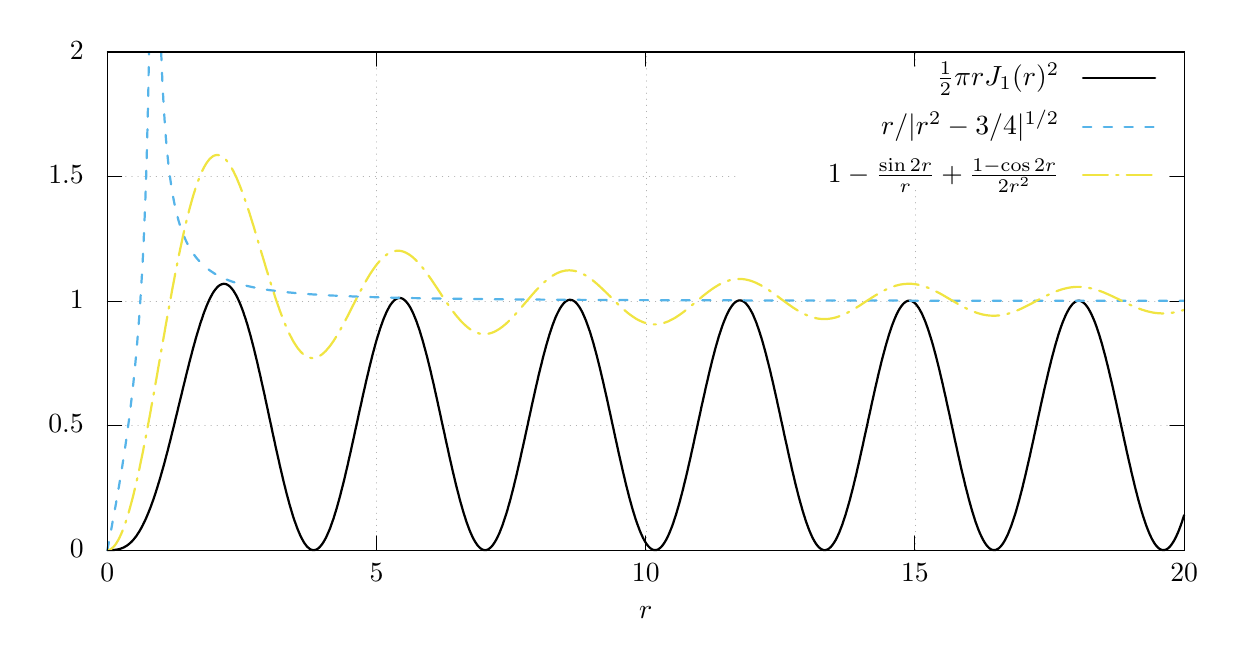
\begin{tikzpicture}[gnuplot]
	%% generated with GNUPLOT 6.0p4 (Lua 5.4; terminal rev. Jun 2020, script rev. 120)
	%% 2026/06/01 15:56:30
	\tikzset{every node/.append style={font={\normalsize}}}
	\path (0.000,0.000) rectangle (15.240,7.620);
	\gpcolor{color=gp lt color axes}
	\gpsetlinetype{gp lt axes}
	\gpsetdashtype{gp dt axes}
	\gpsetlinewidth{0.50}
	\draw[gp path] (1.012,0.985)--(14.687,0.985);
	\gpcolor{color=gp lt color border}
	\gpsetlinetype{gp lt border}
	\gpsetdashtype{gp dt solid}
	\gpsetlinewidth{1.00}
	\draw[gp path] (1.012,0.985)--(1.192,0.985);
	\draw[gp path] (14.687,0.985)--(14.507,0.985);
	\node[gp node right] at (0.828,0.985) {$0$};
	\gpcolor{color=gp lt color axes}
	\gpsetlinetype{gp lt axes}
	\gpsetdashtype{gp dt axes}
	\gpsetlinewidth{0.50}
	\draw[gp path] (1.012,2.567)--(14.687,2.567);
	\gpcolor{color=gp lt color border}
	\gpsetlinetype{gp lt border}
	\gpsetdashtype{gp dt solid}
	\gpsetlinewidth{1.00}
	\draw[gp path] (1.012,2.567)--(1.192,2.567);
	\draw[gp path] (14.687,2.567)--(14.507,2.567);
	\node[gp node right] at (0.828,2.567) {$0.5$};
	\gpcolor{color=gp lt color axes}
	\gpsetlinetype{gp lt axes}
	\gpsetdashtype{gp dt axes}
	\gpsetlinewidth{0.50}
	\draw[gp path] (1.012,4.148)--(14.687,4.148);
	\gpcolor{color=gp lt color border}
	\gpsetlinetype{gp lt border}
	\gpsetdashtype{gp dt solid}
	\gpsetlinewidth{1.00}
	\draw[gp path] (1.012,4.148)--(1.192,4.148);
	\draw[gp path] (14.687,4.148)--(14.507,4.148);
	\node[gp node right] at (0.828,4.148) {$1$};
	\gpcolor{color=gp lt color axes}
	\gpsetlinetype{gp lt axes}
	\gpsetdashtype{gp dt axes}
	\gpsetlinewidth{0.50}
	\draw[gp path] (1.012,5.730)--(8.987,5.730);
	\draw[gp path] (14.503,5.730)--(14.687,5.730);
	\gpcolor{color=gp lt color border}
	\gpsetlinetype{gp lt border}
	\gpsetdashtype{gp dt solid}
	\gpsetlinewidth{1.00}
	\draw[gp path] (1.012,5.730)--(1.192,5.730);
	\draw[gp path] (14.687,5.730)--(14.507,5.730);
	\node[gp node right] at (0.828,5.730) {$1.5$};
	\gpcolor{color=gp lt color axes}
	\gpsetlinetype{gp lt axes}
	\gpsetdashtype{gp dt axes}
	\gpsetlinewidth{0.50}
	\draw[gp path] (1.012,7.311)--(14.687,7.311);
	\gpcolor{color=gp lt color border}
	\gpsetlinetype{gp lt border}
	\gpsetdashtype{gp dt solid}
	\gpsetlinewidth{1.00}
	\draw[gp path] (1.012,7.311)--(1.192,7.311);
	\draw[gp path] (14.687,7.311)--(14.507,7.311);
	\node[gp node right] at (0.828,7.311) {$2$};
	\gpcolor{color=gp lt color axes}
	\gpsetlinetype{gp lt axes}
	\gpsetdashtype{gp dt axes}
	\gpsetlinewidth{0.50}
	\draw[gp path] (1.012,0.985)--(1.012,7.311);
	\gpcolor{color=gp lt color border}
	\gpsetlinetype{gp lt border}
	\gpsetdashtype{gp dt solid}
	\gpsetlinewidth{1.00}
	\draw[gp path] (1.012,0.985)--(1.012,1.165);
	\draw[gp path] (1.012,7.311)--(1.012,7.131);
	\node[gp node center] at (1.012,0.677) {$0$};
	\gpcolor{color=gp lt color axes}
	\gpsetlinetype{gp lt axes}
	\gpsetdashtype{gp dt axes}
	\gpsetlinewidth{0.50}
	\draw[gp path] (4.431,0.985)--(4.431,7.311);
	\gpcolor{color=gp lt color border}
	\gpsetlinetype{gp lt border}
	\gpsetdashtype{gp dt solid}
	\gpsetlinewidth{1.00}
	\draw[gp path] (4.431,0.985)--(4.431,1.165);
	\draw[gp path] (4.431,7.311)--(4.431,7.131);
	\node[gp node center] at (4.431,0.677) {$5$};
	\gpcolor{color=gp lt color axes}
	\gpsetlinetype{gp lt axes}
	\gpsetdashtype{gp dt axes}
	\gpsetlinewidth{0.50}
	\draw[gp path] (7.850,0.985)--(7.850,7.311);
	\gpcolor{color=gp lt color border}
	\gpsetlinetype{gp lt border}
	\gpsetdashtype{gp dt solid}
	\gpsetlinewidth{1.00}
	\draw[gp path] (7.850,0.985)--(7.850,1.165);
	\draw[gp path] (7.850,7.311)--(7.850,7.131);
	\node[gp node center] at (7.850,0.677) {$10$};
	\gpcolor{color=gp lt color axes}
	\gpsetlinetype{gp lt axes}
	\gpsetdashtype{gp dt axes}
	\gpsetlinewidth{0.50}
	\draw[gp path] (11.268,0.985)--(11.268,5.591);
	\draw[gp path] (11.268,7.131)--(11.268,7.311);
	\gpcolor{color=gp lt color border}
	\gpsetlinetype{gp lt border}
	\gpsetdashtype{gp dt solid}
	\gpsetlinewidth{1.00}
	\draw[gp path] (11.268,0.985)--(11.268,1.165);
	\draw[gp path] (11.268,7.311)--(11.268,7.131);
	\node[gp node center] at (11.268,0.677) {$15$};
	\gpcolor{color=gp lt color axes}
	\gpsetlinetype{gp lt axes}
	\gpsetdashtype{gp dt axes}
	\gpsetlinewidth{0.50}
	\draw[gp path] (14.687,0.985)--(14.687,7.311);
	\gpcolor{color=gp lt color border}
	\gpsetlinetype{gp lt border}
	\gpsetdashtype{gp dt solid}
	\gpsetlinewidth{1.00}
	\draw[gp path] (14.687,0.985)--(14.687,1.165);
	\draw[gp path] (14.687,7.311)--(14.687,7.131);
	\node[gp node center] at (14.687,0.677) {$20$};
	\draw[gp path] (1.012,7.311)--(1.012,0.985)--(14.687,0.985)--(14.687,7.311)--cycle;
	\node[gp node right] at (13.219,6.977) {$\frac{1}{2} \pi r \BesselJ{1}(r)^2$};
	\gpcolor{rgb color={0.000,0.000,0.000}}
	\gpsetdashtype{gp dt 1}
	\gpsetlinewidth{2.00}
	\draw[gp path] (13.403,6.977)--(14.319,6.977);
	\draw[gp path] (1.012,0.985)--(1.026,0.985)--(1.039,0.985)--(1.053,0.985)--(1.067,0.986)%
	--(1.080,0.986)--(1.094,0.987)--(1.108,0.988)--(1.122,0.990)--(1.135,0.992)--(1.149,0.995)%
	--(1.163,0.998)--(1.176,1.002)--(1.190,1.007)--(1.204,1.012)--(1.217,1.018)--(1.231,1.025)%
	--(1.245,1.033)--(1.258,1.041)--(1.272,1.051)--(1.286,1.062)--(1.299,1.073)--(1.313,1.086)%
	--(1.327,1.100)--(1.341,1.115)--(1.354,1.131)--(1.368,1.149)--(1.382,1.167)--(1.395,1.187)%
	--(1.409,1.208)--(1.423,1.231)--(1.436,1.254)--(1.450,1.279)--(1.464,1.306)--(1.477,1.333)%
	--(1.491,1.362)--(1.505,1.393)--(1.518,1.424)--(1.532,1.457)--(1.546,1.492)--(1.560,1.527)%
	--(1.573,1.564)--(1.587,1.602)--(1.601,1.641)--(1.614,1.682)--(1.628,1.724)--(1.642,1.767)%
	--(1.655,1.811)--(1.669,1.856)--(1.683,1.902)--(1.696,1.949)--(1.710,1.998)--(1.724,2.047)%
	--(1.738,2.097)--(1.751,2.148)--(1.765,2.200)--(1.779,2.252)--(1.792,2.305)--(1.806,2.359)%
	--(1.820,2.414)--(1.833,2.469)--(1.847,2.524)--(1.861,2.580)--(1.874,2.636)--(1.888,2.692)%
	--(1.902,2.749)--(1.915,2.805)--(1.929,2.862)--(1.943,2.919)--(1.957,2.975)--(1.970,3.032)%
	--(1.984,3.088)--(1.998,3.144)--(2.011,3.199)--(2.025,3.255)--(2.039,3.309)--(2.052,3.363)%
	--(2.066,3.416)--(2.080,3.469)--(2.093,3.520)--(2.107,3.571)--(2.121,3.621)--(2.134,3.669)%
	--(2.148,3.717)--(2.162,3.763)--(2.176,3.808)--(2.189,3.852)--(2.203,3.894)--(2.217,3.935)%
	--(2.230,3.975)--(2.244,4.013)--(2.258,4.049)--(2.271,4.083)--(2.285,4.116)--(2.299,4.147)%
	--(2.312,4.176)--(2.326,4.203)--(2.340,4.228)--(2.353,4.252)--(2.367,4.273)--(2.381,4.292)%
	--(2.395,4.309)--(2.408,4.324)--(2.422,4.337)--(2.436,4.347)--(2.449,4.355)--(2.463,4.361)%
	--(2.477,4.365)--(2.490,4.367)--(2.504,4.366)--(2.518,4.363)--(2.531,4.358)--(2.545,4.350)%
	--(2.559,4.340)--(2.573,4.328)--(2.586,4.314)--(2.600,4.297)--(2.614,4.278)--(2.627,4.257)%
	--(2.641,4.234)--(2.655,4.208)--(2.668,4.181)--(2.682,4.151)--(2.696,4.119)--(2.709,4.086)%
	--(2.723,4.050)--(2.737,4.012)--(2.750,3.972)--(2.764,3.931)--(2.778,3.888)--(2.792,3.843)%
	--(2.805,3.796)--(2.819,3.748)--(2.833,3.698)--(2.846,3.647)--(2.860,3.594)--(2.874,3.540)%
	--(2.887,3.485)--(2.901,3.428)--(2.915,3.371)--(2.928,3.312)--(2.942,3.252)--(2.956,3.192)%
	--(2.969,3.131)--(2.983,3.069)--(2.997,3.007)--(3.011,2.944)--(3.024,2.880)--(3.038,2.817)%
	--(3.052,2.753)--(3.065,2.689)--(3.079,2.625)--(3.093,2.561)--(3.106,2.497)--(3.120,2.433)%
	--(3.134,2.370)--(3.147,2.307)--(3.161,2.245)--(3.175,2.183)--(3.189,2.122)--(3.202,2.061)%
	--(3.216,2.002)--(3.230,1.943)--(3.243,1.886)--(3.257,1.829)--(3.271,1.774)--(3.284,1.720)%
	--(3.298,1.668)--(3.312,1.617)--(3.325,1.567)--(3.339,1.520)--(3.353,1.473)--(3.366,1.429)%
	--(3.380,1.386)--(3.394,1.345)--(3.408,1.307)--(3.421,1.270)--(3.435,1.235)--(3.449,1.202)%
	--(3.462,1.171)--(3.476,1.143)--(3.490,1.117)--(3.503,1.093)--(3.517,1.071)--(3.531,1.052)%
	--(3.544,1.035)--(3.558,1.021)--(3.572,1.009)--(3.585,0.999)--(3.599,0.992)--(3.613,0.987)%
	--(3.627,0.985)--(3.640,0.985)--(3.654,0.988)--(3.668,0.993)--(3.681,1.001)--(3.695,1.011)%
	--(3.709,1.024)--(3.722,1.039)--(3.736,1.056)--(3.750,1.076)--(3.763,1.098)--(3.777,1.122)%
	--(3.791,1.149)--(3.804,1.178)--(3.818,1.209)--(3.832,1.242)--(3.846,1.277)--(3.859,1.315)%
	--(3.873,1.354)--(3.887,1.395)--(3.900,1.438)--(3.914,1.483)--(3.928,1.529)--(3.941,1.577)%
	--(3.955,1.627)--(3.969,1.678)--(3.982,1.731)--(3.996,1.785)--(4.010,1.840)--(4.024,1.896)%
	--(4.037,1.954)--(4.051,2.012)--(4.065,2.071)--(4.078,2.132)--(4.092,2.192)--(4.106,2.254)%
	--(4.119,2.316)--(4.133,2.378)--(4.147,2.441)--(4.160,2.504)--(4.174,2.567)--(4.188,2.630)%
	--(4.201,2.693)--(4.215,2.756)--(4.229,2.818)--(4.243,2.881)--(4.256,2.943)--(4.270,3.004)%
	--(4.284,3.064)--(4.297,3.124)--(4.311,3.183)--(4.325,3.241)--(4.338,3.298)--(4.352,3.354)%
	--(4.366,3.409)--(4.379,3.463)--(4.393,3.515)--(4.407,3.566)--(4.420,3.615)--(4.434,3.663)%
	--(4.448,3.708)--(4.462,3.753)--(4.475,3.795)--(4.489,3.835)--(4.503,3.874)--(4.516,3.911)%
	--(4.530,3.945)--(4.544,3.977)--(4.557,4.008)--(4.571,4.036)--(4.585,4.061)--(4.598,4.085)%
	--(4.612,4.106)--(4.626,4.125)--(4.640,4.141)--(4.653,4.155)--(4.667,4.166)--(4.681,4.175)%
	--(4.694,4.182)--(4.708,4.186)--(4.722,4.187)--(4.735,4.186)--(4.749,4.183)--(4.763,4.177)%
	--(4.776,4.168)--(4.790,4.157)--(4.804,4.144)--(4.817,4.128)--(4.831,4.110)--(4.845,4.089)%
	--(4.859,4.066)--(4.872,4.041)--(4.886,4.013)--(4.900,3.983)--(4.913,3.951)--(4.927,3.917)%
	--(4.941,3.881)--(4.954,3.843)--(4.968,3.802)--(4.982,3.760)--(4.995,3.716)--(5.009,3.671)%
	--(5.023,3.623)--(5.036,3.574)--(5.050,3.523)--(5.064,3.471)--(5.078,3.418)--(5.091,3.363)%
	--(5.105,3.307)--(5.119,3.250)--(5.132,3.192)--(5.146,3.133)--(5.160,3.073)--(5.173,3.012)%
	--(5.187,2.950)--(5.201,2.888)--(5.214,2.826)--(5.228,2.763)--(5.242,2.700)--(5.255,2.636)%
	--(5.269,2.573)--(5.283,2.510)--(5.297,2.446)--(5.310,2.383)--(5.324,2.321)--(5.338,2.258)%
	--(5.351,2.196)--(5.365,2.135)--(5.379,2.075)--(5.392,2.015)--(5.406,1.956)--(5.420,1.898)%
	--(5.433,1.842)--(5.447,1.786)--(5.461,1.732)--(5.475,1.679)--(5.488,1.627)--(5.502,1.577)%
	--(5.516,1.529)--(5.529,1.482)--(5.543,1.437)--(5.557,1.394)--(5.570,1.352)--(5.584,1.313)%
	--(5.598,1.275)--(5.611,1.240)--(5.625,1.207)--(5.639,1.175)--(5.652,1.147)--(5.666,1.120)%
	--(5.680,1.096)--(5.694,1.074)--(5.707,1.054)--(5.721,1.037)--(5.735,1.022)--(5.748,1.010)%
	--(5.762,1.000)--(5.776,0.992)--(5.789,0.988)--(5.803,0.985)--(5.817,0.985)--(5.830,0.988)%
	--(5.844,0.993)--(5.858,1.001)--(5.871,1.011)--(5.885,1.024)--(5.899,1.039)--(5.913,1.057)%
	--(5.926,1.077)--(5.940,1.099)--(5.954,1.124)--(5.967,1.151)--(5.981,1.180)--(5.995,1.211)%
	--(6.008,1.245)--(6.022,1.280)--(6.036,1.318)--(6.049,1.358)--(6.063,1.400)--(6.077,1.443)%
	--(6.091,1.488)--(6.104,1.536)--(6.118,1.584)--(6.132,1.634)--(6.145,1.686)--(6.159,1.739)%
	--(6.173,1.794)--(6.186,1.850)--(6.200,1.906)--(6.214,1.964)--(6.227,2.023)--(6.241,2.083)%
	--(6.255,2.143)--(6.268,2.205)--(6.282,2.267)--(6.296,2.329)--(6.310,2.392)--(6.323,2.454)%
	--(6.337,2.518)--(6.351,2.581)--(6.364,2.644)--(6.378,2.707)--(6.392,2.770)--(6.405,2.833)%
	--(6.419,2.895)--(6.433,2.957)--(6.446,3.018)--(6.460,3.078)--(6.474,3.138)--(6.487,3.197)%
	--(6.501,3.254)--(6.515,3.311)--(6.529,3.366)--(6.542,3.421)--(6.556,3.474)--(6.570,3.525)%
	--(6.583,3.575)--(6.597,3.623)--(6.611,3.670)--(6.624,3.715)--(6.638,3.758)--(6.652,3.800)%
	--(6.665,3.839)--(6.679,3.876)--(6.693,3.912)--(6.706,3.945)--(6.720,3.976)--(6.734,4.004)%
	--(6.748,4.031)--(6.761,4.055)--(6.775,4.077)--(6.789,4.096)--(6.802,4.113)--(6.816,4.128)%
	--(6.830,4.140)--(6.843,4.150)--(6.857,4.157)--(6.871,4.162)--(6.884,4.164)--(6.898,4.163)%
	--(6.912,4.160)--(6.926,4.155)--(6.939,4.147)--(6.953,4.137)--(6.967,4.124)--(6.980,4.108)%
	--(6.994,4.090)--(7.008,4.070)--(7.021,4.048)--(7.035,4.023)--(7.049,3.995)--(7.062,3.966)%
	--(7.076,3.934)--(7.090,3.900)--(7.103,3.864)--(7.117,3.826)--(7.131,3.786)--(7.145,3.745)%
	--(7.158,3.701)--(7.172,3.655)--(7.186,3.608)--(7.199,3.559)--(7.213,3.508)--(7.227,3.456)%
	--(7.240,3.403)--(7.254,3.348)--(7.268,3.292)--(7.281,3.235)--(7.295,3.177)--(7.309,3.118)%
	--(7.322,3.058)--(7.336,2.998)--(7.350,2.936)--(7.364,2.874)--(7.377,2.812)--(7.391,2.749)%
	--(7.405,2.686)--(7.418,2.623)--(7.432,2.559)--(7.446,2.496)--(7.459,2.433)--(7.473,2.370)%
	--(7.487,2.307)--(7.500,2.245)--(7.514,2.183)--(7.528,2.122)--(7.542,2.062)--(7.555,2.002)%
	--(7.569,1.944)--(7.583,1.886)--(7.596,1.829)--(7.610,1.774)--(7.624,1.720)--(7.637,1.667)%
	--(7.651,1.616)--(7.665,1.566)--(7.678,1.518)--(7.692,1.472)--(7.706,1.427)--(7.719,1.384)%
	--(7.733,1.343)--(7.747,1.304)--(7.761,1.267)--(7.774,1.232)--(7.788,1.199)--(7.802,1.168)%
	--(7.815,1.140)--(7.829,1.114)--(7.843,1.090)--(7.856,1.068)--(7.870,1.049)--(7.884,1.033)%
	--(7.897,1.019)--(7.911,1.007)--(7.925,0.998)--(7.938,0.991)--(7.952,0.987)--(7.966,0.985)%
	--(7.980,0.986)--(7.993,0.989)--(8.007,0.995)--(8.021,1.004)--(8.034,1.014)--(8.048,1.028)%
	--(8.062,1.044)--(8.075,1.062)--(8.089,1.083)--(8.103,1.106)--(8.116,1.131)--(8.130,1.159)%
	--(8.144,1.189)--(8.157,1.221)--(8.171,1.255)--(8.185,1.291)--(8.199,1.330)--(8.212,1.370)%
	--(8.226,1.412)--(8.240,1.457)--(8.253,1.503)--(8.267,1.550)--(8.281,1.599)--(8.294,1.650)%
	--(8.308,1.702)--(8.322,1.756)--(8.335,1.811)--(8.349,1.867)--(8.363,1.924)--(8.377,1.983)%
	--(8.390,2.042)--(8.404,2.102)--(8.418,2.163)--(8.431,2.224)--(8.445,2.286)--(8.459,2.349)%
	--(8.472,2.412)--(8.486,2.475)--(8.500,2.538)--(8.513,2.601)--(8.527,2.665)--(8.541,2.728)%
	--(8.554,2.791)--(8.568,2.853)--(8.582,2.915)--(8.596,2.977)--(8.609,3.038)--(8.623,3.098)%
	--(8.637,3.157)--(8.650,3.215)--(8.664,3.273)--(8.678,3.329)--(8.691,3.384)--(8.705,3.437)%
	--(8.719,3.490)--(8.732,3.541)--(8.746,3.590)--(8.760,3.638)--(8.773,3.684)--(8.787,3.728)%
	--(8.801,3.770)--(8.815,3.811)--(8.828,3.849)--(8.842,3.886)--(8.856,3.920)--(8.869,3.952)%
	--(8.883,3.982)--(8.897,4.010)--(8.910,4.035)--(8.924,4.058)--(8.938,4.079)--(8.951,4.097)%
	--(8.965,4.113)--(8.979,4.127)--(8.993,4.138)--(9.006,4.146)--(9.020,4.152)--(9.034,4.156)%
	--(9.047,4.157)--(9.061,4.155)--(9.075,4.151)--(9.088,4.144)--(9.102,4.135)--(9.116,4.123)%
	--(9.129,4.109)--(9.143,4.092)--(9.157,4.073)--(9.170,4.052)--(9.184,4.028)--(9.198,4.002)%
	--(9.212,3.974)--(9.225,3.943)--(9.239,3.910)--(9.253,3.875)--(9.266,3.838)--(9.280,3.799)%
	--(9.294,3.758)--(9.307,3.715)--(9.321,3.671)--(9.335,3.624)--(9.348,3.576)--(9.362,3.526)%
	--(9.376,3.475)--(9.389,3.422)--(9.403,3.368)--(9.417,3.313)--(9.431,3.256)--(9.444,3.199)%
	--(9.458,3.140)--(9.472,3.080)--(9.485,3.020)--(9.499,2.959)--(9.513,2.897)--(9.526,2.835)%
	--(9.540,2.772)--(9.554,2.709)--(9.567,2.646)--(9.581,2.583)--(9.595,2.520)--(9.608,2.456)%
	--(9.622,2.393)--(9.636,2.331)--(9.650,2.268)--(9.663,2.206)--(9.677,2.145)--(9.691,2.084)%
	--(9.704,2.024)--(9.718,1.965)--(9.732,1.907)--(9.745,1.850)--(9.759,1.794)--(9.773,1.740)%
	--(9.786,1.687)--(9.800,1.635)--(9.814,1.584)--(9.828,1.536)--(9.841,1.488)--(9.855,1.443)%
	--(9.869,1.399)--(9.882,1.358)--(9.896,1.318)--(9.910,1.280)--(9.923,1.244)--(9.937,1.211)%
	--(9.951,1.179)--(9.964,1.150)--(9.978,1.123)--(9.992,1.098)--(10.005,1.076)--(10.019,1.056)%
	--(10.033,1.038)--(10.047,1.023)--(10.060,1.011)--(10.074,1.001)--(10.088,0.993)--(10.101,0.988)%
	--(10.115,0.985)--(10.129,0.985)--(10.142,0.988)--(10.156,0.993)--(10.170,1.000)--(10.183,1.010)%
	--(10.197,1.023)--(10.211,1.038)--(10.224,1.055)--(10.238,1.075)--(10.252,1.097)--(10.266,1.122)%
	--(10.279,1.149)--(10.293,1.178)--(10.307,1.209)--(10.320,1.243)--(10.334,1.279)--(10.348,1.316)%
	--(10.361,1.356)--(10.375,1.398)--(10.389,1.441)--(10.402,1.487)--(10.416,1.534)--(10.430,1.583)%
	--(10.444,1.633)--(10.457,1.685)--(10.471,1.738)--(10.485,1.792)--(10.498,1.848)--(10.512,1.905)%
	--(10.526,1.963)--(10.539,2.022)--(10.553,2.082)--(10.567,2.143)--(10.580,2.204)--(10.594,2.266)%
	--(10.608,2.328)--(10.621,2.391)--(10.635,2.454)--(10.649,2.517)--(10.663,2.580)--(10.676,2.644)%
	--(10.690,2.707)--(10.704,2.770)--(10.717,2.832)--(10.731,2.895)--(10.745,2.956)--(10.758,3.017)%
	--(10.772,3.078)--(10.786,3.137)--(10.799,3.196)--(10.813,3.254)--(10.827,3.310)--(10.840,3.365)%
	--(10.854,3.420)--(10.868,3.472)--(10.882,3.524)--(10.895,3.573)--(10.909,3.622)--(10.923,3.668)%
	--(10.936,3.713)--(10.950,3.756)--(10.964,3.797)--(10.977,3.836)--(10.991,3.873)--(11.005,3.908)%
	--(11.018,3.940)--(11.032,3.971)--(11.046,3.999)--(11.059,4.025)--(11.073,4.049)--(11.087,4.071)%
	--(11.101,4.090)--(11.114,4.106)--(11.128,4.120)--(11.142,4.132)--(11.155,4.141)--(11.169,4.148)%
	--(11.183,4.152)--(11.196,4.153)--(11.210,4.152)--(11.224,4.149)--(11.237,4.143)--(11.251,4.134)%
	--(11.265,4.123)--(11.279,4.110)--(11.292,4.094)--(11.306,4.075)--(11.320,4.055)--(11.333,4.031)%
	--(11.347,4.006)--(11.361,3.978)--(11.374,3.948)--(11.388,3.916)--(11.402,3.881)--(11.415,3.845)%
	--(11.429,3.806)--(11.443,3.766)--(11.456,3.723)--(11.470,3.679)--(11.484,3.633)--(11.498,3.585)%
	--(11.511,3.536)--(11.525,3.485)--(11.539,3.432)--(11.552,3.379)--(11.566,3.324)--(11.580,3.267)%
	--(11.593,3.210)--(11.607,3.152)--(11.621,3.092)--(11.634,3.032)--(11.648,2.971)--(11.662,2.910)%
	--(11.675,2.847)--(11.689,2.785)--(11.703,2.722)--(11.717,2.659)--(11.730,2.596)--(11.744,2.532)%
	--(11.758,2.469)--(11.771,2.406)--(11.785,2.343)--(11.799,2.281)--(11.812,2.218)--(11.826,2.157)%
	--(11.840,2.096)--(11.853,2.036)--(11.867,1.977)--(11.881,1.919)--(11.895,1.862)--(11.908,1.805)%
	--(11.922,1.751)--(11.936,1.697)--(11.949,1.645)--(11.963,1.594)--(11.977,1.545)--(11.990,1.498)%
	--(12.004,1.452)--(12.018,1.408)--(12.031,1.366)--(12.045,1.325)--(12.059,1.287)--(12.072,1.251)%
	--(12.086,1.217)--(12.100,1.185)--(12.114,1.155)--(12.127,1.128)--(12.141,1.103)--(12.155,1.080)%
	--(12.168,1.060)--(12.182,1.042)--(12.196,1.026)--(12.209,1.013)--(12.223,1.002)--(12.237,0.994)%
	--(12.250,0.989)--(12.264,0.986)--(12.278,0.985)--(12.291,0.987)--(12.305,0.992)--(12.319,0.999)%
	--(12.333,1.008)--(12.346,1.020)--(12.360,1.035)--(12.374,1.052)--(12.387,1.071)--(12.401,1.093)%
	--(12.415,1.117)--(12.428,1.144)--(12.442,1.172)--(12.456,1.203)--(12.469,1.237)--(12.483,1.272)%
	--(12.497,1.309)--(12.510,1.349)--(12.524,1.390)--(12.538,1.433)--(12.552,1.478)--(12.565,1.525)%
	--(12.579,1.574)--(12.593,1.624)--(12.606,1.675)--(12.620,1.728)--(12.634,1.782)--(12.647,1.838)%
	--(12.661,1.895)--(12.675,1.953)--(12.688,2.011)--(12.702,2.071)--(12.716,2.132)--(12.730,2.193)%
	--(12.743,2.255)--(12.757,2.317)--(12.771,2.380)--(12.784,2.443)--(12.798,2.506)--(12.812,2.569)%
	--(12.825,2.632)--(12.839,2.696)--(12.853,2.759)--(12.866,2.821)--(12.880,2.884)--(12.894,2.945)%
	--(12.907,3.007)--(12.921,3.067)--(12.935,3.127)--(12.949,3.185)--(12.962,3.243)--(12.976,3.300)%
	--(12.990,3.356)--(13.003,3.410)--(13.017,3.463)--(13.031,3.514)--(13.044,3.564)--(13.058,3.613)%
	--(13.072,3.659)--(13.085,3.704)--(13.099,3.748)--(13.113,3.789)--(13.126,3.828)--(13.140,3.866)%
	--(13.154,3.901)--(13.168,3.934)--(13.181,3.965)--(13.195,3.994)--(13.209,4.020)--(13.222,4.044)%
	--(13.236,4.066)--(13.250,4.085)--(13.263,4.102)--(13.277,4.117)--(13.291,4.129)--(13.304,4.138)%
	--(13.318,4.145)--(13.332,4.150)--(13.346,4.152)--(13.359,4.151)--(13.373,4.148)--(13.387,4.142)%
	--(13.400,4.134)--(13.414,4.123)--(13.428,4.110)--(13.441,4.095)--(13.455,4.076)--(13.469,4.056)%
	--(13.482,4.033)--(13.496,4.008)--(13.510,3.980)--(13.523,3.951)--(13.537,3.919)--(13.551,3.885)%
	--(13.565,3.848)--(13.578,3.810)--(13.592,3.770)--(13.606,3.728)--(13.619,3.684)--(13.633,3.638)%
	--(13.647,3.590)--(13.660,3.541)--(13.674,3.490)--(13.688,3.438)--(13.701,3.384)--(13.715,3.330)%
	--(13.729,3.273)--(13.742,3.216)--(13.756,3.158)--(13.770,3.099)--(13.784,3.039)--(13.797,2.978)%
	--(13.811,2.916)--(13.825,2.854)--(13.838,2.792)--(13.852,2.729)--(13.866,2.666)--(13.879,2.602)%
	--(13.893,2.539)--(13.907,2.476)--(13.920,2.413)--(13.934,2.350)--(13.948,2.287)--(13.961,2.225)%
	--(13.975,2.164)--(13.989,2.103)--(14.003,2.043)--(14.016,1.983)--(14.030,1.925)--(14.044,1.868)%
	--(14.057,1.811)--(14.071,1.756)--(14.085,1.703)--(14.098,1.650)--(14.112,1.600)--(14.126,1.550)%
	--(14.139,1.503)--(14.153,1.457)--(14.167,1.412)--(14.181,1.370)--(14.194,1.330)--(14.208,1.291)%
	--(14.222,1.255)--(14.235,1.221)--(14.249,1.188)--(14.263,1.158)--(14.276,1.131)--(14.290,1.105)%
	--(14.304,1.082)--(14.317,1.062)--(14.331,1.043)--(14.345,1.028)--(14.358,1.014)--(14.372,1.003)%
	--(14.386,0.995)--(14.400,0.989)--(14.413,0.986)--(14.427,0.985)--(14.441,0.987)--(14.454,0.991)%
	--(14.468,0.998)--(14.482,1.007)--(14.495,1.019)--(14.509,1.033)--(14.523,1.050)--(14.536,1.069)%
	--(14.550,1.091)--(14.564,1.115)--(14.577,1.141)--(14.591,1.169)--(14.605,1.200)--(14.619,1.233)%
	--(14.632,1.268)--(14.646,1.305)--(14.660,1.345)--(14.673,1.386)--(14.687,1.429);
	\gpcolor{color=gp lt color border}
	\node[gp node right] at (13.219,6.669) { };
	\gpcolor{color=gpbgfillcolor}
	\gpsetlinetype{gp lt plot 4}
	\gpsetdashtype{gp dt solid}
	\gpsetlinewidth{1.00}
	\draw[gp path] (13.403,6.669)--(14.319,6.669);
	\gpcolor{color=gp lt color border}
	\node[gp node right] at (13.219,6.361) {$r/\abs{r^2 - 3/4}^{1/2}$};
	\gpcolor{rgb color={0.337,0.706,0.914}}
	\gpsetlinetype{gp lt border}
	\gpsetdashtype{gp dt 3}
	\gpsetlinewidth{2.00}
	\draw[gp path] (13.403,6.361)--(14.319,6.361);
	\draw[gp path] (1.012,0.985)--(1.026,1.058)--(1.039,1.131)--(1.053,1.205)--(1.067,1.279)%
	--(1.080,1.353)--(1.094,1.428)--(1.108,1.504)--(1.122,1.580)--(1.135,1.658)--(1.149,1.737)%
	--(1.163,1.817)--(1.176,1.898)--(1.190,1.982)--(1.204,2.067)--(1.217,2.154)--(1.231,2.244)%
	--(1.245,2.337)--(1.258,2.432)--(1.272,2.531)--(1.286,2.634)--(1.299,2.741)--(1.313,2.853)%
	--(1.327,2.971)--(1.341,3.094)--(1.354,3.225)--(1.368,3.364)--(1.382,3.512)--(1.395,3.671)%
	--(1.409,3.843)--(1.423,4.030)--(1.436,4.235)--(1.450,4.462)--(1.464,4.717)--(1.477,5.006)%
	--(1.491,5.340)--(1.505,5.733)--(1.518,6.207)--(1.532,6.800)--(1.541,7.311);
	\draw[gp path] (1.695,7.311)--(1.696,7.292)--(1.710,6.956)--(1.724,6.685)--(1.738,6.459)%
	--(1.751,6.269)--(1.765,6.107)--(1.779,5.966)--(1.792,5.842)--(1.806,5.733)--(1.820,5.636)%
	--(1.833,5.549)--(1.847,5.471)--(1.861,5.400)--(1.874,5.336)--(1.888,5.277)--(1.902,5.223)%
	--(1.915,5.173)--(1.929,5.127)--(1.943,5.084)--(1.957,5.045)--(1.970,5.008)--(1.984,4.974)%
	--(1.998,4.942)--(2.011,4.912)--(2.025,4.883)--(2.039,4.857)--(2.052,4.832)--(2.066,4.808)%
	--(2.080,4.786)--(2.093,4.765)--(2.107,4.745)--(2.121,4.726)--(2.134,4.708)--(2.148,4.691)%
	--(2.162,4.675)--(2.176,4.659)--(2.189,4.645)--(2.203,4.631)--(2.217,4.617)--(2.230,4.604)%
	--(2.244,4.592)--(2.258,4.580)--(2.271,4.569)--(2.285,4.558)--(2.299,4.548)--(2.312,4.538)%
	--(2.326,4.528)--(2.340,4.519)--(2.353,4.510)--(2.367,4.501)--(2.381,4.493)--(2.395,4.485)%
	--(2.408,4.478)--(2.422,4.470)--(2.436,4.463)--(2.449,4.456)--(2.463,4.450)--(2.477,4.443)%
	--(2.490,4.437)--(2.504,4.431)--(2.518,4.425)--(2.531,4.420)--(2.545,4.414)--(2.559,4.409)%
	--(2.573,4.404)--(2.586,4.399)--(2.600,4.394)--(2.614,4.389)--(2.627,4.385)--(2.641,4.380)%
	--(2.655,4.376)--(2.668,4.372)--(2.682,4.368)--(2.696,4.364)--(2.709,4.360)--(2.723,4.356)%
	--(2.737,4.353)--(2.750,4.349)--(2.764,4.346)--(2.778,4.342)--(2.792,4.339)--(2.805,4.336)%
	--(2.819,4.333)--(2.833,4.330)--(2.846,4.327)--(2.860,4.324)--(2.874,4.321)--(2.887,4.319)%
	--(2.901,4.316)--(2.915,4.313)--(2.928,4.311)--(2.942,4.308)--(2.956,4.306)--(2.969,4.303)%
	--(2.983,4.301)--(2.997,4.299)--(3.011,4.297)--(3.024,4.295)--(3.038,4.292)--(3.052,4.290)%
	--(3.065,4.288)--(3.079,4.286)--(3.093,4.284)--(3.106,4.283)--(3.120,4.281)--(3.134,4.279)%
	--(3.147,4.277)--(3.161,4.275)--(3.175,4.274)--(3.189,4.272)--(3.202,4.270)--(3.216,4.269)%
	--(3.230,4.267)--(3.243,4.266)--(3.257,4.264)--(3.271,4.263)--(3.284,4.261)--(3.298,4.260)%
	--(3.312,4.258)--(3.325,4.257)--(3.339,4.256)--(3.353,4.254)--(3.366,4.253)--(3.380,4.252)%
	--(3.394,4.251)--(3.408,4.249)--(3.421,4.248)--(3.435,4.247)--(3.449,4.246)--(3.462,4.245)%
	--(3.476,4.243)--(3.490,4.242)--(3.503,4.241)--(3.517,4.240)--(3.531,4.239)--(3.544,4.238)%
	--(3.558,4.237)--(3.572,4.236)--(3.585,4.235)--(3.599,4.234)--(3.613,4.233)--(3.627,4.232)%
	--(3.640,4.231)--(3.654,4.231)--(3.668,4.230)--(3.681,4.229)--(3.695,4.228)--(3.709,4.227)%
	--(3.722,4.226)--(3.736,4.225)--(3.750,4.225)--(3.763,4.224)--(3.777,4.223)--(3.791,4.222)%
	--(3.804,4.222)--(3.818,4.221)--(3.832,4.220)--(3.846,4.219)--(3.859,4.219)--(3.873,4.218)%
	--(3.887,4.217)--(3.900,4.217)--(3.914,4.216)--(3.928,4.215)--(3.941,4.215)--(3.955,4.214)%
	--(3.969,4.213)--(3.982,4.213)--(3.996,4.212)--(4.010,4.212)--(4.024,4.211)--(4.037,4.210)%
	--(4.051,4.210)--(4.065,4.209)--(4.078,4.209)--(4.092,4.208)--(4.106,4.208)--(4.119,4.207)%
	--(4.133,4.207)--(4.147,4.206)--(4.160,4.205)--(4.174,4.205)--(4.188,4.204)--(4.201,4.204)%
	--(4.215,4.203)--(4.229,4.203)--(4.243,4.203)--(4.256,4.202)--(4.270,4.202)--(4.284,4.201)%
	--(4.297,4.201)--(4.311,4.200)--(4.325,4.200)--(4.338,4.199)--(4.352,4.199)--(4.366,4.198)%
	--(4.379,4.198)--(4.393,4.198)--(4.407,4.197)--(4.420,4.197)--(4.434,4.196)--(4.448,4.196)%
	--(4.462,4.196)--(4.475,4.195)--(4.489,4.195)--(4.503,4.195)--(4.516,4.194)--(4.530,4.194)%
	--(4.544,4.193)--(4.557,4.193)--(4.571,4.193)--(4.585,4.192)--(4.598,4.192)--(4.612,4.192)%
	--(4.626,4.191)--(4.640,4.191)--(4.653,4.191)--(4.667,4.190)--(4.681,4.190)--(4.694,4.190)%
	--(4.708,4.189)--(4.722,4.189)--(4.735,4.189)--(4.749,4.188)--(4.763,4.188)--(4.776,4.188)%
	--(4.790,4.188)--(4.804,4.187)--(4.817,4.187)--(4.831,4.187)--(4.845,4.186)--(4.859,4.186)%
	--(4.872,4.186)--(4.886,4.186)--(4.900,4.185)--(4.913,4.185)--(4.927,4.185)--(4.941,4.185)%
	--(4.954,4.184)--(4.968,4.184)--(4.982,4.184)--(4.995,4.184)--(5.009,4.183)--(5.023,4.183)%
	--(5.036,4.183)--(5.050,4.183)--(5.064,4.182)--(5.078,4.182)--(5.091,4.182)--(5.105,4.182)%
	--(5.119,4.181)--(5.132,4.181)--(5.146,4.181)--(5.160,4.181)--(5.173,4.181)--(5.187,4.180)%
	--(5.201,4.180)--(5.214,4.180)--(5.228,4.180)--(5.242,4.179)--(5.255,4.179)--(5.269,4.179)%
	--(5.283,4.179)--(5.297,4.179)--(5.310,4.178)--(5.324,4.178)--(5.338,4.178)--(5.351,4.178)%
	--(5.365,4.178)--(5.379,4.177)--(5.392,4.177)--(5.406,4.177)--(5.420,4.177)--(5.433,4.177)%
	--(5.447,4.177)--(5.461,4.176)--(5.475,4.176)--(5.488,4.176)--(5.502,4.176)--(5.516,4.176)%
	--(5.529,4.176)--(5.543,4.175)--(5.557,4.175)--(5.570,4.175)--(5.584,4.175)--(5.598,4.175)%
	--(5.611,4.175)--(5.625,4.174)--(5.639,4.174)--(5.652,4.174)--(5.666,4.174)--(5.680,4.174)%
	--(5.694,4.174)--(5.707,4.173)--(5.721,4.173)--(5.735,4.173)--(5.748,4.173)--(5.762,4.173)%
	--(5.776,4.173)--(5.789,4.173)--(5.803,4.172)--(5.817,4.172)--(5.830,4.172)--(5.844,4.172)%
	--(5.858,4.172)--(5.871,4.172)--(5.885,4.172)--(5.899,4.171)--(5.913,4.171)--(5.926,4.171)%
	--(5.940,4.171)--(5.954,4.171)--(5.967,4.171)--(5.981,4.171)--(5.995,4.171)--(6.008,4.170)%
	--(6.022,4.170)--(6.036,4.170)--(6.049,4.170)--(6.063,4.170)--(6.077,4.170)--(6.091,4.170)%
	--(6.104,4.170)--(6.118,4.169)--(6.132,4.169)--(6.145,4.169)--(6.159,4.169)--(6.173,4.169)%
	--(6.186,4.169)--(6.200,4.169)--(6.214,4.169)--(6.227,4.169)--(6.241,4.168)--(6.255,4.168)%
	--(6.268,4.168)--(6.282,4.168)--(6.296,4.168)--(6.310,4.168)--(6.323,4.168)--(6.337,4.168)%
	--(6.351,4.168)--(6.364,4.168)--(6.378,4.167)--(6.392,4.167)--(6.405,4.167)--(6.419,4.167)%
	--(6.433,4.167)--(6.446,4.167)--(6.460,4.167)--(6.474,4.167)--(6.487,4.167)--(6.501,4.167)%
	--(6.515,4.166)--(6.529,4.166)--(6.542,4.166)--(6.556,4.166)--(6.570,4.166)--(6.583,4.166)%
	--(6.597,4.166)--(6.611,4.166)--(6.624,4.166)--(6.638,4.166)--(6.652,4.166)--(6.665,4.165)%
	--(6.679,4.165)--(6.693,4.165)--(6.706,4.165)--(6.720,4.165)--(6.734,4.165)--(6.748,4.165)%
	--(6.761,4.165)--(6.775,4.165)--(6.789,4.165)--(6.802,4.165)--(6.816,4.165)--(6.830,4.165)%
	--(6.843,4.164)--(6.857,4.164)--(6.871,4.164)--(6.884,4.164)--(6.898,4.164)--(6.912,4.164)%
	--(6.926,4.164)--(6.939,4.164)--(6.953,4.164)--(6.967,4.164)--(6.980,4.164)--(6.994,4.164)%
	--(7.008,4.164)--(7.021,4.163)--(7.035,4.163)--(7.049,4.163)--(7.062,4.163)--(7.076,4.163)%
	--(7.090,4.163)--(7.103,4.163)--(7.117,4.163)--(7.131,4.163)--(7.145,4.163)--(7.158,4.163)%
	--(7.172,4.163)--(7.186,4.163)--(7.199,4.163)--(7.213,4.163)--(7.227,4.162)--(7.240,4.162)%
	--(7.254,4.162)--(7.268,4.162)--(7.281,4.162)--(7.295,4.162)--(7.309,4.162)--(7.322,4.162)%
	--(7.336,4.162)--(7.350,4.162)--(7.364,4.162)--(7.377,4.162)--(7.391,4.162)--(7.405,4.162)%
	--(7.418,4.162)--(7.432,4.162)--(7.446,4.161)--(7.459,4.161)--(7.473,4.161)--(7.487,4.161)%
	--(7.500,4.161)--(7.514,4.161)--(7.528,4.161)--(7.542,4.161)--(7.555,4.161)--(7.569,4.161)%
	--(7.583,4.161)--(7.596,4.161)--(7.610,4.161)--(7.624,4.161)--(7.637,4.161)--(7.651,4.161)%
	--(7.665,4.161)--(7.678,4.161)--(7.692,4.161)--(7.706,4.160)--(7.719,4.160)--(7.733,4.160)%
	--(7.747,4.160)--(7.761,4.160)--(7.774,4.160)--(7.788,4.160)--(7.802,4.160)--(7.815,4.160)%
	--(7.829,4.160)--(7.843,4.160)--(7.856,4.160)--(7.870,4.160)--(7.884,4.160)--(7.897,4.160)%
	--(7.911,4.160)--(7.925,4.160)--(7.938,4.160)--(7.952,4.160)--(7.966,4.160)--(7.980,4.159)%
	--(7.993,4.159)--(8.007,4.159)--(8.021,4.159)--(8.034,4.159)--(8.048,4.159)--(8.062,4.159)%
	--(8.075,4.159)--(8.089,4.159)--(8.103,4.159)--(8.116,4.159)--(8.130,4.159)--(8.144,4.159)%
	--(8.157,4.159)--(8.171,4.159)--(8.185,4.159)--(8.199,4.159)--(8.212,4.159)--(8.226,4.159)%
	--(8.240,4.159)--(8.253,4.159)--(8.267,4.159)--(8.281,4.159)--(8.294,4.159)--(8.308,4.158)%
	--(8.322,4.158)--(8.335,4.158)--(8.349,4.158)--(8.363,4.158)--(8.377,4.158)--(8.390,4.158)%
	--(8.404,4.158)--(8.418,4.158)--(8.431,4.158)--(8.445,4.158)--(8.459,4.158)--(8.472,4.158)%
	--(8.486,4.158)--(8.500,4.158)--(8.513,4.158)--(8.527,4.158)--(8.541,4.158)--(8.554,4.158)%
	--(8.568,4.158)--(8.582,4.158)--(8.596,4.158)--(8.609,4.158)--(8.623,4.158)--(8.637,4.158)%
	--(8.650,4.158)--(8.664,4.158)--(8.678,4.157)--(8.691,4.157)--(8.705,4.157)--(8.719,4.157)%
	--(8.732,4.157)--(8.746,4.157)--(8.760,4.157)--(8.773,4.157)--(8.787,4.157)--(8.801,4.157)%
	--(8.815,4.157)--(8.828,4.157)--(8.842,4.157)--(8.856,4.157)--(8.869,4.157)--(8.883,4.157)%
	--(8.897,4.157)--(8.910,4.157)--(8.924,4.157)--(8.938,4.157)--(8.951,4.157)--(8.965,4.157)%
	--(8.979,4.157)--(8.993,4.157)--(9.006,4.157)--(9.020,4.157)--(9.034,4.157)--(9.047,4.157)%
	--(9.061,4.157)--(9.075,4.157)--(9.088,4.157)--(9.102,4.157)--(9.116,4.156)--(9.129,4.156)%
	--(9.143,4.156)--(9.157,4.156)--(9.170,4.156)--(9.184,4.156)--(9.198,4.156)--(9.212,4.156)%
	--(9.225,4.156)--(9.239,4.156)--(9.253,4.156)--(9.266,4.156)--(9.280,4.156)--(9.294,4.156)%
	--(9.307,4.156)--(9.321,4.156)--(9.335,4.156)--(9.348,4.156)--(9.362,4.156)--(9.376,4.156)%
	--(9.389,4.156)--(9.403,4.156)--(9.417,4.156)--(9.431,4.156)--(9.444,4.156)--(9.458,4.156)%
	--(9.472,4.156)--(9.485,4.156)--(9.499,4.156)--(9.513,4.156)--(9.526,4.156)--(9.540,4.156)%
	--(9.554,4.156)--(9.567,4.156)--(9.581,4.156)--(9.595,4.156)--(9.608,4.156)--(9.622,4.156)%
	--(9.636,4.155)--(9.650,4.155)--(9.663,4.155)--(9.677,4.155)--(9.691,4.155)--(9.704,4.155)%
	--(9.718,4.155)--(9.732,4.155)--(9.745,4.155)--(9.759,4.155)--(9.773,4.155)--(9.786,4.155)%
	--(9.800,4.155)--(9.814,4.155)--(9.828,4.155)--(9.841,4.155)--(9.855,4.155)--(9.869,4.155)%
	--(9.882,4.155)--(9.896,4.155)--(9.910,4.155)--(9.923,4.155)--(9.937,4.155)--(9.951,4.155)%
	--(9.964,4.155)--(9.978,4.155)--(9.992,4.155)--(10.005,4.155)--(10.019,4.155)--(10.033,4.155)%
	--(10.047,4.155)--(10.060,4.155)--(10.074,4.155)--(10.088,4.155)--(10.101,4.155)--(10.115,4.155)%
	--(10.129,4.155)--(10.142,4.155)--(10.156,4.155)--(10.170,4.155)--(10.183,4.155)--(10.197,4.155)%
	--(10.211,4.155)--(10.224,4.155)--(10.238,4.155)--(10.252,4.155)--(10.266,4.154)--(10.279,4.154)%
	--(10.293,4.154)--(10.307,4.154)--(10.320,4.154)--(10.334,4.154)--(10.348,4.154)--(10.361,4.154)%
	--(10.375,4.154)--(10.389,4.154)--(10.402,4.154)--(10.416,4.154)--(10.430,4.154)--(10.444,4.154)%
	--(10.457,4.154)--(10.471,4.154)--(10.485,4.154)--(10.498,4.154)--(10.512,4.154)--(10.526,4.154)%
	--(10.539,4.154)--(10.553,4.154)--(10.567,4.154)--(10.580,4.154)--(10.594,4.154)--(10.608,4.154)%
	--(10.621,4.154)--(10.635,4.154)--(10.649,4.154)--(10.663,4.154)--(10.676,4.154)--(10.690,4.154)%
	--(10.704,4.154)--(10.717,4.154)--(10.731,4.154)--(10.745,4.154)--(10.758,4.154)--(10.772,4.154)%
	--(10.786,4.154)--(10.799,4.154)--(10.813,4.154)--(10.827,4.154)--(10.840,4.154)--(10.854,4.154)%
	--(10.868,4.154)--(10.882,4.154)--(10.895,4.154)--(10.909,4.154)--(10.923,4.154)--(10.936,4.154)%
	--(10.950,4.154)--(10.964,4.154)--(10.977,4.154)--(10.991,4.154)--(11.005,4.154)--(11.018,4.154)%
	--(11.032,4.154)--(11.046,4.154)--(11.059,4.154)--(11.073,4.153)--(11.087,4.153)--(11.101,4.153)%
	--(11.114,4.153)--(11.128,4.153)--(11.142,4.153)--(11.155,4.153)--(11.169,4.153)--(11.183,4.153)%
	--(11.196,4.153)--(11.210,4.153)--(11.224,4.153)--(11.237,4.153)--(11.251,4.153)--(11.265,4.153)%
	--(11.279,4.153)--(11.292,4.153)--(11.306,4.153)--(11.320,4.153)--(11.333,4.153)--(11.347,4.153)%
	--(11.361,4.153)--(11.374,4.153)--(11.388,4.153)--(11.402,4.153)--(11.415,4.153)--(11.429,4.153)%
	--(11.443,4.153)--(11.456,4.153)--(11.470,4.153)--(11.484,4.153)--(11.498,4.153)--(11.511,4.153)%
	--(11.525,4.153)--(11.539,4.153)--(11.552,4.153)--(11.566,4.153)--(11.580,4.153)--(11.593,4.153)%
	--(11.607,4.153)--(11.621,4.153)--(11.634,4.153)--(11.648,4.153)--(11.662,4.153)--(11.675,4.153)%
	--(11.689,4.153)--(11.703,4.153)--(11.717,4.153)--(11.730,4.153)--(11.744,4.153)--(11.758,4.153)%
	--(11.771,4.153)--(11.785,4.153)--(11.799,4.153)--(11.812,4.153)--(11.826,4.153)--(11.840,4.153)%
	--(11.853,4.153)--(11.867,4.153)--(11.881,4.153)--(11.895,4.153)--(11.908,4.153)--(11.922,4.153)%
	--(11.936,4.153)--(11.949,4.153)--(11.963,4.153)--(11.977,4.153)--(11.990,4.153)--(12.004,4.153)%
	--(12.018,4.153)--(12.031,4.153)--(12.045,4.153)--(12.059,4.153)--(12.072,4.153)--(12.086,4.153)%
	--(12.100,4.153)--(12.114,4.153)--(12.127,4.152)--(12.141,4.152)--(12.155,4.152)--(12.168,4.152)%
	--(12.182,4.152)--(12.196,4.152)--(12.209,4.152)--(12.223,4.152)--(12.237,4.152)--(12.250,4.152)%
	--(12.264,4.152)--(12.278,4.152)--(12.291,4.152)--(12.305,4.152)--(12.319,4.152)--(12.333,4.152)%
	--(12.346,4.152)--(12.360,4.152)--(12.374,4.152)--(12.387,4.152)--(12.401,4.152)--(12.415,4.152)%
	--(12.428,4.152)--(12.442,4.152)--(12.456,4.152)--(12.469,4.152)--(12.483,4.152)--(12.497,4.152)%
	--(12.510,4.152)--(12.524,4.152)--(12.538,4.152)--(12.552,4.152)--(12.565,4.152)--(12.579,4.152)%
	--(12.593,4.152)--(12.606,4.152)--(12.620,4.152)--(12.634,4.152)--(12.647,4.152)--(12.661,4.152)%
	--(12.675,4.152)--(12.688,4.152)--(12.702,4.152)--(12.716,4.152)--(12.730,4.152)--(12.743,4.152)%
	--(12.757,4.152)--(12.771,4.152)--(12.784,4.152)--(12.798,4.152)--(12.812,4.152)--(12.825,4.152)%
	--(12.839,4.152)--(12.853,4.152)--(12.866,4.152)--(12.880,4.152)--(12.894,4.152)--(12.907,4.152)%
	--(12.921,4.152)--(12.935,4.152)--(12.949,4.152)--(12.962,4.152)--(12.976,4.152)--(12.990,4.152)%
	--(13.003,4.152)--(13.017,4.152)--(13.031,4.152)--(13.044,4.152)--(13.058,4.152)--(13.072,4.152)%
	--(13.085,4.152)--(13.099,4.152)--(13.113,4.152)--(13.126,4.152)--(13.140,4.152)--(13.154,4.152)%
	--(13.168,4.152)--(13.181,4.152)--(13.195,4.152)--(13.209,4.152)--(13.222,4.152)--(13.236,4.152)%
	--(13.250,4.152)--(13.263,4.152)--(13.277,4.152)--(13.291,4.152)--(13.304,4.152)--(13.318,4.152)%
	--(13.332,4.152)--(13.346,4.152)--(13.359,4.152)--(13.373,4.152)--(13.387,4.152)--(13.400,4.152)%
	--(13.414,4.152)--(13.428,4.152)--(13.441,4.152)--(13.455,4.152)--(13.469,4.152)--(13.482,4.152)%
	--(13.496,4.152)--(13.510,4.152)--(13.523,4.152)--(13.537,4.152)--(13.551,4.152)--(13.565,4.152)%
	--(13.578,4.152)--(13.592,4.152)--(13.606,4.152)--(13.619,4.151)--(13.633,4.151)--(13.647,4.151)%
	--(13.660,4.151)--(13.674,4.151)--(13.688,4.151)--(13.701,4.151)--(13.715,4.151)--(13.729,4.151)%
	--(13.742,4.151)--(13.756,4.151)--(13.770,4.151)--(13.784,4.151)--(13.797,4.151)--(13.811,4.151)%
	--(13.825,4.151)--(13.838,4.151)--(13.852,4.151)--(13.866,4.151)--(13.879,4.151)--(13.893,4.151)%
	--(13.907,4.151)--(13.920,4.151)--(13.934,4.151)--(13.948,4.151)--(13.961,4.151)--(13.975,4.151)%
	--(13.989,4.151)--(14.003,4.151)--(14.016,4.151)--(14.030,4.151)--(14.044,4.151)--(14.057,4.151)%
	--(14.071,4.151)--(14.085,4.151)--(14.098,4.151)--(14.112,4.151)--(14.126,4.151)--(14.139,4.151)%
	--(14.153,4.151)--(14.167,4.151)--(14.181,4.151)--(14.194,4.151)--(14.208,4.151)--(14.222,4.151)%
	--(14.235,4.151)--(14.249,4.151)--(14.263,4.151)--(14.276,4.151)--(14.290,4.151)--(14.304,4.151)%
	--(14.317,4.151)--(14.331,4.151)--(14.345,4.151)--(14.358,4.151)--(14.372,4.151)--(14.386,4.151)%
	--(14.400,4.151)--(14.413,4.151)--(14.427,4.151)--(14.441,4.151)--(14.454,4.151)--(14.468,4.151)%
	--(14.482,4.151)--(14.495,4.151)--(14.509,4.151)--(14.523,4.151)--(14.536,4.151)--(14.550,4.151)%
	--(14.564,4.151)--(14.577,4.151)--(14.591,4.151)--(14.605,4.151)--(14.619,4.151)--(14.632,4.151)%
	--(14.646,4.151)--(14.660,4.151)--(14.673,4.151)--(14.687,4.151);
	\gpcolor{color=gp lt color border}
	\node[gp node right] at (13.219,6.053) { };
	\gpcolor{color=gpbgfillcolor}
	\gpsetlinetype{gp lt plot 4}
	\gpsetdashtype{gp dt solid}
	\gpsetlinewidth{1.00}
	\draw[gp path] (13.403,6.053)--(14.319,6.053);
	\gpcolor{color=gp lt color border}
	\node[gp node right] at (13.219,5.745) {$1 - \frac{\sin{2r}}{r} + \frac{1 - \cos{2r}}{2r^2}$};
	\gpcolor{rgb color={0.941,0.894,0.259}}
	\gpsetlinetype{gp lt border}
	\gpsetdashtype{gp dt 5}
	\gpsetlinewidth{2.00}
	\draw[gp path] (13.403,5.745)--(14.319,5.745);
	\draw[gp path] (1.026,0.986)--(1.039,0.990)--(1.053,0.996)--(1.067,1.005)--(1.080,1.017)%
	--(1.094,1.030)--(1.108,1.047)--(1.122,1.066)--(1.135,1.087)--(1.149,1.111)--(1.163,1.137)%
	--(1.176,1.165)--(1.190,1.196)--(1.204,1.229)--(1.217,1.265)--(1.231,1.302)--(1.245,1.342)%
	--(1.258,1.384)--(1.272,1.428)--(1.286,1.474)--(1.299,1.522)--(1.313,1.573)--(1.327,1.625)%
	--(1.341,1.679)--(1.354,1.734)--(1.368,1.792)--(1.382,1.851)--(1.395,1.912)--(1.409,1.974)%
	--(1.423,2.038)--(1.436,2.103)--(1.450,2.170)--(1.464,2.237)--(1.477,2.306)--(1.491,2.377)%
	--(1.505,2.448)--(1.518,2.520)--(1.532,2.593)--(1.546,2.667)--(1.560,2.742)--(1.573,2.818)%
	--(1.587,2.894)--(1.601,2.970)--(1.614,3.048)--(1.628,3.125)--(1.642,3.203)--(1.655,3.281)%
	--(1.669,3.359)--(1.683,3.437)--(1.696,3.515)--(1.710,3.594)--(1.724,3.672)--(1.738,3.749)%
	--(1.751,3.827)--(1.765,3.904)--(1.779,3.980)--(1.792,4.056)--(1.806,4.132)--(1.820,4.206)%
	--(1.833,4.280)--(1.847,4.353)--(1.861,4.425)--(1.874,4.497)--(1.888,4.567)--(1.902,4.636)%
	--(1.915,4.704)--(1.929,4.770)--(1.943,4.836)--(1.957,4.900)--(1.970,4.963)--(1.984,5.024)%
	--(1.998,5.084)--(2.011,5.142)--(2.025,5.198)--(2.039,5.253)--(2.052,5.306)--(2.066,5.358)%
	--(2.080,5.408)--(2.093,5.455)--(2.107,5.502)--(2.121,5.546)--(2.134,5.588)--(2.148,5.628)%
	--(2.162,5.666)--(2.176,5.703)--(2.189,5.737)--(2.203,5.769)--(2.217,5.800)--(2.230,5.828)%
	--(2.244,5.854)--(2.258,5.878)--(2.271,5.900)--(2.285,5.919)--(2.299,5.937)--(2.312,5.953)%
	--(2.326,5.966)--(2.340,5.977)--(2.353,5.987)--(2.367,5.994)--(2.381,5.999)--(2.395,6.002)%
	--(2.408,6.003)--(2.422,6.002)--(2.436,5.999)--(2.449,5.995)--(2.463,5.988)--(2.477,5.979)%
	--(2.490,5.968)--(2.504,5.956)--(2.518,5.942)--(2.531,5.926)--(2.545,5.908)--(2.559,5.888)%
	--(2.573,5.867)--(2.586,5.844)--(2.600,5.820)--(2.614,5.794)--(2.627,5.767)--(2.641,5.738)%
	--(2.655,5.708)--(2.668,5.676)--(2.682,5.643)--(2.696,5.609)--(2.709,5.574)--(2.723,5.538)%
	--(2.737,5.501)--(2.750,5.462)--(2.764,5.423)--(2.778,5.383)--(2.792,5.342)--(2.805,5.300)%
	--(2.819,5.258)--(2.833,5.214)--(2.846,5.171)--(2.860,5.127)--(2.874,5.082)--(2.887,5.037)%
	--(2.901,4.991)--(2.915,4.946)--(2.928,4.900)--(2.942,4.854)--(2.956,4.808)--(2.969,4.762)%
	--(2.983,4.716)--(2.997,4.670)--(3.011,4.624)--(3.024,4.578)--(3.038,4.533)--(3.052,4.488)%
	--(3.065,4.443)--(3.079,4.399)--(3.093,4.355)--(3.106,4.312)--(3.120,4.269)--(3.134,4.227)%
	--(3.147,4.186)--(3.161,4.145)--(3.175,4.105)--(3.189,4.066)--(3.202,4.028)--(3.216,3.991)%
	--(3.230,3.954)--(3.243,3.919)--(3.257,3.884)--(3.271,3.851)--(3.284,3.819)--(3.298,3.788)%
	--(3.312,3.758)--(3.325,3.729)--(3.339,3.702)--(3.353,3.675)--(3.366,3.650)--(3.380,3.626)%
	--(3.394,3.604)--(3.408,3.582)--(3.421,3.562)--(3.435,3.544)--(3.449,3.527)--(3.462,3.511)%
	--(3.476,3.496)--(3.490,3.483)--(3.503,3.471)--(3.517,3.460)--(3.531,3.451)--(3.544,3.443)%
	--(3.558,3.437)--(3.572,3.432)--(3.585,3.428)--(3.599,3.425)--(3.613,3.424)--(3.627,3.424)%
	--(3.640,3.426)--(3.654,3.428)--(3.668,3.432)--(3.681,3.438)--(3.695,3.444)--(3.709,3.452)%
	--(3.722,3.460)--(3.736,3.470)--(3.750,3.481)--(3.763,3.493)--(3.777,3.506)--(3.791,3.520)%
	--(3.804,3.536)--(3.818,3.552)--(3.832,3.569)--(3.846,3.586)--(3.859,3.605)--(3.873,3.625)%
	--(3.887,3.645)--(3.900,3.666)--(3.914,3.688)--(3.928,3.710)--(3.941,3.733)--(3.955,3.756)%
	--(3.969,3.781)--(3.982,3.805)--(3.996,3.830)--(4.010,3.855)--(4.024,3.881)--(4.037,3.907)%
	--(4.051,3.934)--(4.065,3.960)--(4.078,3.987)--(4.092,4.014)--(4.106,4.041)--(4.119,4.068)%
	--(4.133,4.095)--(4.147,4.122)--(4.160,4.149)--(4.174,4.175)--(4.188,4.202)--(4.201,4.228)%
	--(4.215,4.255)--(4.229,4.281)--(4.243,4.306)--(4.256,4.331)--(4.270,4.356)--(4.284,4.381)%
	--(4.297,4.405)--(4.311,4.428)--(4.325,4.451)--(4.338,4.474)--(4.352,4.496)--(4.366,4.517)%
	--(4.379,4.537)--(4.393,4.557)--(4.407,4.577)--(4.420,4.595)--(4.434,4.613)--(4.448,4.630)%
	--(4.462,4.646)--(4.475,4.661)--(4.489,4.676)--(4.503,4.690)--(4.516,4.703)--(4.530,4.715)%
	--(4.544,4.726)--(4.557,4.736)--(4.571,4.745)--(4.585,4.754)--(4.598,4.761)--(4.612,4.768)%
	--(4.626,4.773)--(4.640,4.778)--(4.653,4.782)--(4.667,4.784)--(4.681,4.786)--(4.694,4.787)%
	--(4.708,4.787)--(4.722,4.786)--(4.735,4.785)--(4.749,4.782)--(4.763,4.778)--(4.776,4.774)%
	--(4.790,4.768)--(4.804,4.762)--(4.817,4.755)--(4.831,4.747)--(4.845,4.739)--(4.859,4.729)%
	--(4.872,4.719)--(4.886,4.708)--(4.900,4.696)--(4.913,4.684)--(4.927,4.671)--(4.941,4.657)%
	--(4.954,4.643)--(4.968,4.628)--(4.982,4.612)--(4.995,4.596)--(5.009,4.580)--(5.023,4.563)%
	--(5.036,4.545)--(5.050,4.527)--(5.064,4.509)--(5.078,4.490)--(5.091,4.471)--(5.105,4.451)%
	--(5.119,4.432)--(5.132,4.412)--(5.146,4.392)--(5.160,4.371)--(5.173,4.351)--(5.187,4.330)%
	--(5.201,4.310)--(5.214,4.289)--(5.228,4.268)--(5.242,4.247)--(5.255,4.227)--(5.269,4.206)%
	--(5.283,4.185)--(5.297,4.165)--(5.310,4.145)--(5.324,4.125)--(5.338,4.105)--(5.351,4.086)%
	--(5.365,4.066)--(5.379,4.047)--(5.392,4.029)--(5.406,4.010)--(5.420,3.993)--(5.433,3.975)%
	--(5.447,3.958)--(5.461,3.942)--(5.475,3.926)--(5.488,3.910)--(5.502,3.895)--(5.516,3.881)%
	--(5.529,3.867)--(5.543,3.853)--(5.557,3.841)--(5.570,3.829)--(5.584,3.817)--(5.598,3.806)%
	--(5.611,3.796)--(5.625,3.787)--(5.639,3.778)--(5.652,3.770)--(5.666,3.763)--(5.680,3.756)%
	--(5.694,3.750)--(5.707,3.745)--(5.721,3.740)--(5.735,3.736)--(5.748,3.733)--(5.762,3.731)%
	--(5.776,3.729)--(5.789,3.728)--(5.803,3.728)--(5.817,3.729)--(5.830,3.730)--(5.844,3.732)%
	--(5.858,3.735)--(5.871,3.738)--(5.885,3.742)--(5.899,3.747)--(5.913,3.752)--(5.926,3.758)%
	--(5.940,3.765)--(5.954,3.772)--(5.967,3.780)--(5.981,3.788)--(5.995,3.797)--(6.008,3.807)%
	--(6.022,3.817)--(6.036,3.827)--(6.049,3.839)--(6.063,3.850)--(6.077,3.862)--(6.091,3.875)%
	--(6.104,3.888)--(6.118,3.901)--(6.132,3.915)--(6.145,3.929)--(6.159,3.943)--(6.173,3.957)%
	--(6.186,3.972)--(6.200,3.987)--(6.214,4.003)--(6.227,4.018)--(6.241,4.034)--(6.255,4.050)%
	--(6.268,4.066)--(6.282,4.082)--(6.296,4.098)--(6.310,4.114)--(6.323,4.130)--(6.337,4.146)%
	--(6.351,4.162)--(6.364,4.178)--(6.378,4.194)--(6.392,4.210)--(6.405,4.226)--(6.419,4.241)%
	--(6.433,4.257)--(6.446,4.272)--(6.460,4.287)--(6.474,4.302)--(6.487,4.316)--(6.501,4.330)%
	--(6.515,4.344)--(6.529,4.357)--(6.542,4.370)--(6.556,4.383)--(6.570,4.395)--(6.583,4.407)%
	--(6.597,4.419)--(6.611,4.429)--(6.624,4.440)--(6.638,4.450)--(6.652,4.460)--(6.665,4.469)%
	--(6.679,4.477)--(6.693,4.485)--(6.706,4.493)--(6.720,4.500)--(6.734,4.506)--(6.748,4.512)%
	--(6.761,4.517)--(6.775,4.522)--(6.789,4.526)--(6.802,4.529)--(6.816,4.532)--(6.830,4.535)%
	--(6.843,4.536)--(6.857,4.537)--(6.871,4.538)--(6.884,4.538)--(6.898,4.537)--(6.912,4.536)%
	--(6.926,4.534)--(6.939,4.532)--(6.953,4.529)--(6.967,4.526)--(6.980,4.522)--(6.994,4.517)%
	--(7.008,4.512)--(7.021,4.506)--(7.035,4.500)--(7.049,4.494)--(7.062,4.487)--(7.076,4.479)%
	--(7.090,4.471)--(7.103,4.462)--(7.117,4.453)--(7.131,4.444)--(7.145,4.434)--(7.158,4.424)%
	--(7.172,4.414)--(7.186,4.403)--(7.199,4.392)--(7.213,4.380)--(7.227,4.369)--(7.240,4.357)%
	--(7.254,4.344)--(7.268,4.332)--(7.281,4.319)--(7.295,4.306)--(7.309,4.293)--(7.322,4.280)%
	--(7.336,4.267)--(7.350,4.253)--(7.364,4.240)--(7.377,4.226)--(7.391,4.213)--(7.405,4.199)%
	--(7.418,4.185)--(7.432,4.172)--(7.446,4.158)--(7.459,4.145)--(7.473,4.132)--(7.487,4.118)%
	--(7.500,4.105)--(7.514,4.092)--(7.528,4.079)--(7.542,4.067)--(7.555,4.054)--(7.569,4.042)%
	--(7.583,4.030)--(7.596,4.019)--(7.610,4.007)--(7.624,3.996)--(7.637,3.985)--(7.651,3.975)%
	--(7.665,3.965)--(7.678,3.955)--(7.692,3.946)--(7.706,3.937)--(7.719,3.928)--(7.733,3.920)%
	--(7.747,3.912)--(7.761,3.905)--(7.774,3.898)--(7.788,3.892)--(7.802,3.886)--(7.815,3.880)%
	--(7.829,3.875)--(7.843,3.871)--(7.856,3.867)--(7.870,3.863)--(7.884,3.860)--(7.897,3.857)%
	--(7.911,3.855)--(7.925,3.854)--(7.938,3.853)--(7.952,3.852)--(7.966,3.852)--(7.980,3.852)%
	--(7.993,3.853)--(8.007,3.855)--(8.021,3.857)--(8.034,3.859)--(8.048,3.862)--(8.062,3.865)%
	--(8.075,3.869)--(8.089,3.873)--(8.103,3.878)--(8.116,3.883)--(8.130,3.888)--(8.144,3.894)%
	--(8.157,3.901)--(8.171,3.908)--(8.185,3.915)--(8.199,3.922)--(8.212,3.930)--(8.226,3.938)%
	--(8.240,3.947)--(8.253,3.956)--(8.267,3.965)--(8.281,3.974)--(8.294,3.984)--(8.308,3.994)%
	--(8.322,4.004)--(8.335,4.014)--(8.349,4.025)--(8.363,4.035)--(8.377,4.046)--(8.390,4.057)%
	--(8.404,4.068)--(8.418,4.080)--(8.431,4.091)--(8.445,4.103)--(8.459,4.114)--(8.472,4.126)%
	--(8.486,4.137)--(8.500,4.149)--(8.513,4.160)--(8.527,4.172)--(8.541,4.183)--(8.554,4.194)%
	--(8.568,4.206)--(8.582,4.217)--(8.596,4.228)--(8.609,4.238)--(8.623,4.249)--(8.637,4.260)%
	--(8.650,4.270)--(8.664,4.280)--(8.678,4.290)--(8.691,4.300)--(8.705,4.309)--(8.719,4.318)%
	--(8.732,4.327)--(8.746,4.335)--(8.760,4.344)--(8.773,4.352)--(8.787,4.359)--(8.801,4.366)%
	--(8.815,4.373)--(8.828,4.380)--(8.842,4.386)--(8.856,4.392)--(8.869,4.397)--(8.883,4.402)%
	--(8.897,4.406)--(8.910,4.411)--(8.924,4.414)--(8.938,4.418)--(8.951,4.421)--(8.965,4.423)%
	--(8.979,4.425)--(8.993,4.427)--(9.006,4.428)--(9.020,4.429)--(9.034,4.429)--(9.047,4.429)%
	--(9.061,4.428)--(9.075,4.427)--(9.088,4.426)--(9.102,4.424)--(9.116,4.422)--(9.129,4.419)%
	--(9.143,4.416)--(9.157,4.413)--(9.170,4.409)--(9.184,4.405)--(9.198,4.400)--(9.212,4.395)%
	--(9.225,4.390)--(9.239,4.384)--(9.253,4.378)--(9.266,4.372)--(9.280,4.365)--(9.294,4.358)%
	--(9.307,4.351)--(9.321,4.343)--(9.335,4.335)--(9.348,4.327)--(9.362,4.319)--(9.376,4.310)%
	--(9.389,4.302)--(9.403,4.293)--(9.417,4.284)--(9.431,4.274)--(9.444,4.265)--(9.458,4.255)%
	--(9.472,4.245)--(9.485,4.236)--(9.499,4.226)--(9.513,4.216)--(9.526,4.206)--(9.540,4.196)%
	--(9.554,4.185)--(9.567,4.175)--(9.581,4.165)--(9.595,4.155)--(9.608,4.145)--(9.622,4.135)%
	--(9.636,4.125)--(9.650,4.115)--(9.663,4.105)--(9.677,4.096)--(9.691,4.086)--(9.704,4.077)%
	--(9.718,4.067)--(9.732,4.058)--(9.745,4.049)--(9.759,4.041)--(9.773,4.032)--(9.786,4.024)%
	--(9.800,4.016)--(9.814,4.008)--(9.828,4.001)--(9.841,3.994)--(9.855,3.987)--(9.869,3.980)%
	--(9.882,3.974)--(9.896,3.968)--(9.910,3.962)--(9.923,3.957)--(9.937,3.952)--(9.951,3.947)%
	--(9.964,3.943)--(9.978,3.939)--(9.992,3.935)--(10.005,3.932)--(10.019,3.929)--(10.033,3.926)%
	--(10.047,3.924)--(10.060,3.923)--(10.074,3.921)--(10.088,3.920)--(10.101,3.920)--(10.115,3.919)%
	--(10.129,3.920)--(10.142,3.920)--(10.156,3.921)--(10.170,3.922)--(10.183,3.924)--(10.197,3.926)%
	--(10.211,3.928)--(10.224,3.931)--(10.238,3.934)--(10.252,3.937)--(10.266,3.941)--(10.279,3.945)%
	--(10.293,3.950)--(10.307,3.955)--(10.320,3.960)--(10.334,3.965)--(10.348,3.971)--(10.361,3.977)%
	--(10.375,3.983)--(10.389,3.989)--(10.402,3.996)--(10.416,4.003)--(10.430,4.010)--(10.444,4.017)%
	--(10.457,4.025)--(10.471,4.033)--(10.485,4.041)--(10.498,4.049)--(10.512,4.057)--(10.526,4.065)%
	--(10.539,4.074)--(10.553,4.082)--(10.567,4.091)--(10.580,4.100)--(10.594,4.109)--(10.608,4.118)%
	--(10.621,4.127)--(10.635,4.136)--(10.649,4.145)--(10.663,4.154)--(10.676,4.162)--(10.690,4.171)%
	--(10.704,4.180)--(10.717,4.189)--(10.731,4.198)--(10.745,4.206)--(10.758,4.215)--(10.772,4.223)%
	--(10.786,4.231)--(10.799,4.240)--(10.813,4.248)--(10.827,4.255)--(10.840,4.263)--(10.854,4.270)%
	--(10.868,4.278)--(10.882,4.285)--(10.895,4.291)--(10.909,4.298)--(10.923,4.304)--(10.936,4.310)%
	--(10.950,4.316)--(10.964,4.322)--(10.977,4.327)--(10.991,4.332)--(11.005,4.336)--(11.018,4.341)%
	--(11.032,4.345)--(11.046,4.348)--(11.059,4.352)--(11.073,4.355)--(11.087,4.358)--(11.101,4.360)%
	--(11.114,4.362)--(11.128,4.364)--(11.142,4.365)--(11.155,4.366)--(11.169,4.367)--(11.183,4.368)%
	--(11.196,4.368)--(11.210,4.367)--(11.224,4.367)--(11.237,4.366)--(11.251,4.364)--(11.265,4.363)%
	--(11.279,4.361)--(11.292,4.359)--(11.306,4.356)--(11.320,4.353)--(11.333,4.350)--(11.347,4.346)%
	--(11.361,4.342)--(11.374,4.338)--(11.388,4.334)--(11.402,4.329)--(11.415,4.324)--(11.429,4.319)%
	--(11.443,4.314)--(11.456,4.308)--(11.470,4.302)--(11.484,4.296)--(11.498,4.290)--(11.511,4.283)%
	--(11.525,4.276)--(11.539,4.269)--(11.552,4.262)--(11.566,4.255)--(11.580,4.248)--(11.593,4.240)%
	--(11.607,4.233)--(11.621,4.225)--(11.634,4.217)--(11.648,4.209)--(11.662,4.201)--(11.675,4.193)%
	--(11.689,4.185)--(11.703,4.177)--(11.717,4.169)--(11.730,4.161)--(11.744,4.153)--(11.758,4.145)%
	--(11.771,4.137)--(11.785,4.129)--(11.799,4.121)--(11.812,4.113)--(11.826,4.105)--(11.840,4.098)%
	--(11.853,4.090)--(11.867,4.083)--(11.881,4.075)--(11.895,4.068)--(11.908,4.061)--(11.922,4.054)%
	--(11.936,4.048)--(11.949,4.041)--(11.963,4.035)--(11.977,4.029)--(11.990,4.023)--(12.004,4.017)%
	--(12.018,4.012)--(12.031,4.007)--(12.045,4.002)--(12.059,3.997)--(12.072,3.993)--(12.086,3.989)%
	--(12.100,3.985)--(12.114,3.981)--(12.127,3.978)--(12.141,3.975)--(12.155,3.972)--(12.168,3.970)%
	--(12.182,3.968)--(12.196,3.966)--(12.209,3.965)--(12.223,3.963)--(12.237,3.963)--(12.250,3.962)%
	--(12.264,3.962)--(12.278,3.962)--(12.291,3.962)--(12.305,3.963)--(12.319,3.964)--(12.333,3.965)%
	--(12.346,3.967)--(12.360,3.968)--(12.374,3.971)--(12.387,3.973)--(12.401,3.976)--(12.415,3.979)%
	--(12.428,3.982)--(12.442,3.985)--(12.456,3.989)--(12.469,3.993)--(12.483,3.998)--(12.497,4.002)%
	--(12.510,4.007)--(12.524,4.012)--(12.538,4.017)--(12.552,4.022)--(12.565,4.028)--(12.579,4.034)%
	--(12.593,4.040)--(12.606,4.046)--(12.620,4.052)--(12.634,4.059)--(12.647,4.065)--(12.661,4.072)%
	--(12.675,4.079)--(12.688,4.086)--(12.702,4.093)--(12.716,4.100)--(12.730,4.107)--(12.743,4.114)%
	--(12.757,4.121)--(12.771,4.129)--(12.784,4.136)--(12.798,4.143)--(12.812,4.151)--(12.825,4.158)%
	--(12.839,4.165)--(12.853,4.173)--(12.866,4.180)--(12.880,4.187)--(12.894,4.194)--(12.907,4.201)%
	--(12.921,4.208)--(12.935,4.215)--(12.949,4.221)--(12.962,4.228)--(12.976,4.234)--(12.990,4.241)%
	--(13.003,4.247)--(13.017,4.253)--(13.031,4.259)--(13.044,4.264)--(13.058,4.270)--(13.072,4.275)%
	--(13.085,4.280)--(13.099,4.285)--(13.113,4.289)--(13.126,4.294)--(13.140,4.298)--(13.154,4.302)%
	--(13.168,4.305)--(13.181,4.309)--(13.195,4.312)--(13.209,4.315)--(13.222,4.317)--(13.236,4.320)%
	--(13.250,4.322)--(13.263,4.323)--(13.277,4.325)--(13.291,4.326)--(13.304,4.327)--(13.318,4.328)%
	--(13.332,4.328)--(13.346,4.328)--(13.359,4.328)--(13.373,4.328)--(13.387,4.327)--(13.400,4.326)%
	--(13.414,4.325)--(13.428,4.323)--(13.441,4.321)--(13.455,4.319)--(13.469,4.317)--(13.482,4.314)%
	--(13.496,4.311)--(13.510,4.308)--(13.523,4.305)--(13.537,4.301)--(13.551,4.297)--(13.565,4.293)%
	--(13.578,4.289)--(13.592,4.285)--(13.606,4.280)--(13.619,4.275)--(13.633,4.270)--(13.647,4.265)%
	--(13.660,4.260)--(13.674,4.254)--(13.688,4.248)--(13.701,4.242)--(13.715,4.236)--(13.729,4.230)%
	--(13.742,4.224)--(13.756,4.218)--(13.770,4.211)--(13.784,4.205)--(13.797,4.198)--(13.811,4.192)%
	--(13.825,4.185)--(13.838,4.179)--(13.852,4.172)--(13.866,4.165)--(13.879,4.158)--(13.893,4.152)%
	--(13.907,4.145)--(13.920,4.138)--(13.934,4.132)--(13.948,4.125)--(13.961,4.118)--(13.975,4.112)%
	--(13.989,4.105)--(14.003,4.099)--(14.016,4.093)--(14.030,4.087)--(14.044,4.081)--(14.057,4.075)%
	--(14.071,4.069)--(14.085,4.064)--(14.098,4.058)--(14.112,4.053)--(14.126,4.048)--(14.139,4.043)%
	--(14.153,4.038)--(14.167,4.034)--(14.181,4.029)--(14.194,4.025)--(14.208,4.021)--(14.222,4.018)%
	--(14.235,4.014)--(14.249,4.011)--(14.263,4.008)--(14.276,4.005)--(14.290,4.002)--(14.304,4.000)%
	--(14.317,3.998)--(14.331,3.996)--(14.345,3.995)--(14.358,3.993)--(14.372,3.992)--(14.386,3.992)%
	--(14.400,3.991)--(14.413,3.991)--(14.427,3.991)--(14.441,3.991)--(14.454,3.992)--(14.468,3.992)%
	--(14.482,3.993)--(14.495,3.995)--(14.509,3.996)--(14.523,3.998)--(14.536,4.000)--(14.550,4.002)%
	--(14.564,4.005)--(14.577,4.007)--(14.591,4.010)--(14.605,4.013)--(14.619,4.017)--(14.632,4.020)%
	--(14.646,4.024)--(14.660,4.028)--(14.673,4.032)--(14.687,4.037);
	\gpcolor{color=gp lt color border}
	\gpsetdashtype{gp dt solid}
	\gpsetlinewidth{1.00}
	\draw[gp path] (1.012,7.311)--(1.012,0.985)--(14.687,0.985)--(14.687,7.311)--cycle;
	\node[gp node center,rotate=-270.0] at (0.138,4.148) {$$};
	\node[gp node center] at (7.849,0.215) {$r$};
	%% coordinates of the plot area
	\gpdefrectangularnode{gp plot 1}{\pgfpoint{1.012cm}{0.985cm}}{\pgfpoint{14.687cm}{7.311cm}}
\end{tikzpicture}


		\caption{The graphs of the functions appearing in \eqref{eq:upper bounds for nu=1}.}
		\label{fig:graph}
	\end{figure}
	
	In addition, we establish a dimension-comparison result for the free Schr\"{o}dinger equation on \recordmath{\R^d} and \recordmath{\R^{d+1}} by using Theorem \ref{thm:main thm}. 
	Briefly, we have
	\begin{equation}
\recorddisplay{
	\Constd{d+1} \leq 2 \Constd{d} 
	}
\end{equation}
	for every \recordmath{d \geq 2}, where \recordmath{\Constd{d}} and \recordmath{\Constd{d+1}} denote the optimal constants of a certain inequality on \recordmath{\R^d} and \recordmath{\R^{d+1}}, respectively.
	See Section \ref{section:application} for details.	
	\section{Proof of Theorem \ref{thm:main thm}} \label{section:proof}
	Our proof is based on three classical identities for the Bessel functions: the Wronskian identity, \citeauthor{Wat1944}'s formula \cite[Eq.~(5) in Section 13.73]{Wat1944}, and \citeauthor{Nic1910}'s formula \cite[Eqs.~(33), (34)]{Nic1910}.
	For each \recordmath{(\mu, \nu) \in \R^2}, we define \recordmath{\crossmunu{\mu}{\nu} \colon \intervaloo{0}{\infty} \to \R} by
	\begin{equation} \label{eq:cross product}
		\crossmunu{\mu}{\nu}(r) \coloneqq \det \begin{pmatrix}
			\BesselJ{\mu} & \BesselJ{\nu} \\
			\BesselY{\mu} & \BesselY{\nu}
		\end{pmatrix}
		=
		\BesselJ{\mu}(r) \BesselY{\nu}(r) - \BesselJ{\nu}(r) \BesselY{\mu}(r) ,
	\end{equation}
	that is, a cross product of \recordmath{\BesselJ{}} and \recordmath{\BesselY{}}.
	Then we have the following.
	\begin{proposition}[Wronskian identity] \label{prop:Wronskian}
		Let \recordmath{\nu \in \R} and \recordmath{r \in \intervaloo{0}{\infty}}.
		Then we have
		\begin{equation}
\recorddisplay{ \label{eq:Wronskian}
			\crossmunu{\nu+1/2}{\nu-1/2}(r) = \frac{2}{\pi r} .
		}
\end{equation}
	\end{proposition}
	\begin{proposition}[\citeauthor{Wat1944}'s formula%
		\footnote{Some references (e.g.~\citet[6.617.1]{GR2014}) present \citeauthor{Wat1944}'s formula \eqref{eq:Watson} with the wrong sign in the exponential.}%
] \label{prop:Watson}
		Let \recordmath{\mu \in \intervaloo{-1}{1}}, \recordmath{\nu \in \R}, and \recordmath{r \in \intervaloo{0}{\infty}}.
		Then we have
		\begin{equation}
\recorddisplay{ \label{eq:Watson}
			\crossmunu{\mu+\nu}{\nu}(r) = \frac{4 \sin( \mu \pi )}{\pi^2} \int_{s \in \intervaloo{0}{\infty}} \BesselK{\mu}(2 r \sinh{s}) \exp( - (\mu + 2\nu) s ) \, ds , 
		}
\end{equation}
		where \recordmath{\BesselK{\mu}} is the modified Bessel function of the second kind of order \recordmath{\mu}.
	\end{proposition}
	\begin{proposition}[\citeauthor{Nic1910}'s formula]
		Let \recordmath{\nu \in \R} and \recordmath{r \in \intervaloo{0}{\infty}}.
		Then we have
		\begin{equation}
\recorddisplay{ \label{eq:Nicholson}
			\BesselJ{\nu}(r)^2 + \BesselY{\nu}(r)^2 = \frac{8}{\pi^2} \int_{s \in \intervaloo{0}{\infty}} \BesselK{0}(2 r \sinh{s}) \cosh( 2 \nu s ) \, ds .
		}
\end{equation}
	\end{proposition}
	Since \recordmath{\BesselK{\nu}} is positive on \recordmath{\intervaloo{0}{\infty}} for every \recordmath{\nu \in \R}, 
	we see that the identities \eqref{eq:Watson} and \eqref{eq:Nicholson} imply the following, respectively.
	\begin{corollary} \label{cor:Watson}
		Let \recordmath{\mu \in \intervaloo{0}{1}} and \recordmath{r \in \intervaloo{0}{\infty}}. Then the function
		\begin{equation}
\recorddisplay{
			\nu \longmapsto \crossmunu{\mu+\nu}{\nu}(r)
		}
\end{equation}
		is positive and strictly decreasing on \recordmath{\R}.
	\end{corollary}
	\begin{corollary} \label{cor:Nicholson}
		Let \recordmath{r \in \intervaloo{0}{\infty}}.
		Then the function
		\begin{equation}
\recorddisplay{
			\nu \longmapsto \BesselJ{\nu}(r)^2 + \BesselY{\nu}(r)^2 
		}
\end{equation}
		is even on \recordmath{\R} and strictly increasing on \recordmath{\intervalco{0}{\infty}}.
	\end{corollary}
	Now we prove Theorem \ref{thm:main thm} by using Proposition \ref{prop:Wronskian} and Corollaries \ref{cor:Watson}, \ref{cor:Nicholson}.  
	\begin{proof}[Proof of Theorem \ref{thm:main thm}]
		Using the Wronskian identity \eqref{eq:Wronskian} and Cramer's rule, we obtain
		\begin{equation}
			\frac{2}{\pi r}
			\begin{pmatrix}
				\BesselJ{\mu + \nu}(r) \\
				\BesselY{\mu + \nu}(r)
			\end{pmatrix}
			= \crossmunu{\nu+1/2}{\mu + \nu}(r)
			\begin{pmatrix}
				\BesselJ{\nu-1/2}(r) \\
				\BesselY{\nu-1/2}(r)
			\end{pmatrix}
			+ \crossmunu{\mu + \nu}{\nu-1/2}(r)
			\begin{pmatrix}
				\BesselJ{\nu+1/2}(r) \\
				\BesselY{\nu+1/2}(r)
			\end{pmatrix} ,
		\end{equation} 
		so that
		\begin{equation}
\recorddisplay{
			\frac{2}{\pi r} \BesselJY{\mu+\nu}(r) = \crossmunu{\nu+1/2}{\mu + \nu}(r) \BesselJY{\nu-1/2}(r) + \crossmunu{\mu + \nu}{\nu-1/2}(r) \BesselJY{\nu+1/2}(r) .
		}
\end{equation}
		Thus, applying the Cauchy--Schwarz inequality, we get
		\begin{equation}
\recorddisplay{
		\mleft(\frac{2}{\pi r}\mright)^2 \abs{\BesselJY{\mu+\nu}(r)}^2 \leq (\crossmunu{\nu+1/2}{\mu + \nu}(r)^2 + \crossmunu{\mu + \nu}{\nu-1/2}(r)^2) ( \abs{\BesselJY{\nu-1/2}(r)}^2 + \abs{\BesselJY{\nu+1/2}(r)}^2 ) .
		}
\end{equation}
			We also note that \recordmath{\crossmunu{\nu+1/2}{\nu-1/2}(r) \ne 0} (which follows from the Wronskian identity \eqref{eq:Wronskian}) and the assumption \recordmath{(a, b) \ne (0, 0)} imply that 
		\begin{equation}
\recorddisplay{
			\abs{\BesselJY{\nu-1/2}(r)}^2 + \abs{\BesselJY{\nu+1/2}(r)}^2 > 0 .
		}
\end{equation}
		Therefore, it suffices to show that 
		\begin{equation}
\recorddisplay{
			\crossmunu{\nu+1/2}{\mu + \nu}(r)^2 + \crossmunu{\mu + \nu}{\nu-1/2}(r)^2 < \mleft(\frac{2}{\pi r}\mright)^2
		}
\end{equation}
		holds.
		Moreover, Corollary \ref{cor:Watson} gives us
		\begin{align}
			\recorddisplay{0 < \crossmunu{(1/2-\mu) + \mu + \nu}{\mu + \nu}(r)
} &\recorddisplay{\leq \crossmunu{(1/2-\mu) + \mu}{\mu}(r) ,
} \\
			\recorddisplay{0 < \crossmunu{\mu + \nu}{\nu-1/2}(r)
} &\recorddisplay{\leq \crossmunu{\mu}{-1/2}(r) ,
} 
		\end{align}
		so that it is reduced to
		\begin{equation}
\recorddisplay{ \label{eq:sufficient for L=1}
			\crossmunu{1/2}{\mu}(r)^2 + \crossmunu{\mu}{-1/2}(r)^2 < \mleft(\frac{2}{\pi r}\mright)^2 .
		}
\end{equation}
		Now observe that the left-hand side can be simplified as
		\begin{equation}
\recorddisplay{
			\crossmunu{1/2}{\mu}(r)^2 + \crossmunu{\mu}{-1/2}(r)^2 = \frac{2}{\pi r} \mleft( \BesselJ{\mu}(r)^2 + \BesselY{\mu}(r)^2 \mright) 
		}
\end{equation}
		by substituting
		\begin{equation}
\recorddisplay{
			\BesselJ{-1/2}(r) = - \BesselY{1/2}(r) = \mleft( \frac{2}{\pi r} \mright)^{1/2} \cos{r} , \quad \BesselJ{1/2}(r) = \BesselY{-1/2}(r) = \mleft( \frac{2}{\pi r} \mright)^{1/2} \sin{r} .
		}
\end{equation}
		Then we get
		\begin{equation}
\recorddisplay{
			\BesselJ{\mu}(r)^2 + \BesselY{\mu}(r)^2 < \BesselJ{1/2}(r)^2 + \BesselY{1/2}(r)^2 = \frac{2}{\pi r} 
		}
\end{equation}
		by Corollary \ref{cor:Nicholson}, since \recordmath{\mu \in \intervaloo{-1/2}{1/2}}.
		This completes the proof.
	\end{proof}
	\section{Application to optimal constants of smoothing estimates} \label{section:application}
	Let \recordmath{\Hamiltonianfree \coloneqq - \Laplacian} be the Schr\"{o}dinger operator of a free particle on \recordmath{\R^d}. Then it is well known that the so-called smoothing estimate
\begin{equation}
\recorddisplay{ \label{eq:smoothing free}
	\int_{(x, t) \in \R^d \times \R} w(\abs{x}) \abs{ \psi(\Hamiltonianfree) e^{- i t \Hamiltonianfree} u_0(x) }^2 \, dx \, dt \leq C \norm{u_0}_{L^2(\R^d)}^{2} 
}
\end{equation}
holds for a suitable pair of functions \recordmath{w, \psi \colon \intervaloo{0}{\infty} \to \intervalco{0}{\infty}}, for example,
\begin{alignat}{8}
	&d \geq 3,  \quad && \quad && ( w(r), \psi(s) ) = ( &&(1+r^2)^{-1}, \quad&&(1+s)^{1/4} &&) ,
	\label{eq:type A} 
\end{alignat}
which is due to \citet[Theorem 2]{KY1989}. The inequality \eqref{eq:smoothing free} is usually referred to as a smoothing estimate.
Hereinafter, we always assume that \recordmath{w} and \recordmath{\psi} are non-negative Borel measurable functions defined on \recordmath{\intervaloo{0}{\infty}}.
Now let \recordmath{\Constwpd{w}{\psi}{d} \in \intervalcc{0}{\infty}} be the optimal constant of the inequality \eqref{eq:smoothing free}, 
that is,
\begin{equation}
\recorddisplay{
	\Constwpd{w}{\psi}{d} \coloneqq \sup_{u_0 \in L^2(\R^d) \setminus \{0\}} \frac{1}{\norm{u_0}_{L^2(\R^d)}^{2}} \int_{(x, t) \in \R^d \times \R} w(\abs{x}) \abs{ \psi(\Hamiltonianfree) e^{- i t \Hamiltonianfree} u_0(x) }^2 \, dx \, dt .
}
\end{equation}
\citet[Theorem 4.1]{Wal2002} established the following formula for the optimal constant. 
\begin{theorem}[{\cite[Theorem 4.1]{Wal2002}}] \label{thm:Walther}
	Let \recordmath{w \colon \intervaloo{0}{\infty} \to \intervalco{0}{\infty}}.
	For each \recordmath{\nu \in \R}, we define \recordmath{\Tnu{\nu} w \colon \intervaloo{0}{\infty} \to \intervalcc{0}{\infty}} by
	\begin{equation}
\recorddisplay{ \label{eq:Tnu}
		\Tnu{\nu}w(s) \coloneqq \pi \int_{r \in \intervaloo{0}{\infty}} r s \BesselJ{\nu}(rs)^2 w(r) \, dr .
	}
\end{equation}
	Then, for every \recordmath{d \geq 2} and \recordmath{\psi \colon \intervaloo{0}{\infty} \to \intervalco{0}{\infty}}, we have
	\begin{equation}
\recorddisplay{ \label{eq:Walther}
		\Constwpd{w}{\psi}{d} = \sup_{k \in \Z_{\geq 0}} \esssup_{s \in \intervaloo{0}{\infty}} s^{-1} \psi(s^2)^2 \Tnu{k+d/2-1}w(s) .
	}
\end{equation}
\end{theorem}
Notice that \citeauthor{Wal2002}'s formula immediately implies
\begin{equation}
\recorddisplay{ \label{eq:d+2 vs d}
	\Constwpd{w}{\psi}{d+2} \leq \Constwpd{w}{\psi}{d}
}
\end{equation}
for every \recordmath{d \geq 2} and \recordmath{w, \psi \colon \intervaloo{0}{\infty} \to \intervalco{0}{\infty}}, since
\begin{equation}
\recorddisplay{
	\Constwpd{w}{\psi}{d+2} = \sup_{k \in \Z_{\geq 0}} \esssup_{s \in \intervaloo{0}{\infty}} s^{-1} \psi(s^2)^2 \Tnu{k+(d+2)/2-1}w(s) = \sup_{k \in \Z_{\geq 1}} \esssup_{s \in \intervaloo{0}{\infty}} s^{-1} \psi(s^2)^2 \Tnu{k+d/2-1}w(s) .
}
\end{equation}
Therefore, it is natural to ask if we have
\begin{equation}
\recorddisplay{
	\Constwpd{w}{\psi}{d+1} \lesssim \Constwpd{w}{\psi}{d} .
}
\end{equation}
Our Theorem \ref{thm:main thm} gives an affirmative answer with an explicit constant.
In fact, Theorem \ref{thm:main thm} implies
\begin{equation}
\recorddisplay{
	\Tnu{\nu}w(s) \leq \Tnu{\nu-1/2}w(s) + \Tnu{\nu+1/2}w(s) \leq 2 \max\{ \Tnu{\nu-1/2}w(s) , \, \Tnu{\nu+1/2}w(s) \}
}
\end{equation}
for every \recordmath{w \colon \intervaloo{0}{\infty} \to \intervalco{0}{\infty}}, \recordmath{\nu \in \intervalco{0}{\infty}}, and \recordmath{s \in \intervaloo{0}{\infty}}.
Combining this inequality with \citeauthor{Wal2002}'s formula \eqref{eq:Walther}, we obtain
\begin{equation}
\recorddisplay{ \label{eq:d+1 vs d with const 2}
	\Constwpd{w}{\psi}{d+1} \leq 2 \Constwpd{w}{\psi}{d} .
}
\end{equation}
A related refinement is obtained by comparing these constants with the optimal constant
for the Dirac smoothing estimate.
Let \recordmath{\HamiltonianDirac{m}} be the Dirac operator of a free particle with mass \recordmath{m \in \intervalco{0}{\infty}} on \recordmath{\R^d}, 
and let \recordmath{\ConstwpdDirac{w}{\psi}{d}{m} \in \intervalcc{0}{\infty}} be the optimal constant of the inequality
\begin{equation}
\recorddisplay{ \label{eq:smoothing Dirac}
	\int_{(x, t) \in \R^d \times \R} w(\abs{x}) \abs{ \abs{\HamiltonianDirac{m}}^{-1/2} \psi(\Hamiltonianfree) e^{- i t \HamiltonianDirac{m}} u_0(x) }^2 \, dx \, dt \leq C \norm{u_0}_{L^2(\R^d, \C^\dimN)}^{2} ,
}
\end{equation}
where \recordmath{\dimN \coloneqq 2^{\lfloor (d+1)/2 \rfloor}}.
\citet{Suz2025} showed the following analogue of Theorem \ref{thm:Walther}.
\begin{theorem}[{\cite[Theorem 1.5]{Suz2025}}]
	Let \recordmath{m \in \intervalco{0}{\infty}} and \recordmath{w \colon \intervaloo{0}{\infty} \to \intervalco{0}{\infty}}.
	For each \recordmath{\nu \in \R}, we define \recordmath{\TnumDirac{\nu}{m} w \colon \intervaloo{0}{\infty} \to \intervalcc{0}{\infty}} by
	\begin{equation}
\recorddisplay{ \label{eq:Tnu Dirac}
	\TnumDirac{\nu}{m}w(s) \coloneqq \Tnu{\nu}w(s) + \Tnu{\nu+1}w(s) + \frac{m}{(m^2+s^2)^{1/2}} \abs{ \Tnu{\nu}w(s) - \Tnu{\nu+1}w(s) } ,
	}
\end{equation}
	where \recordmath{\Tnu{\nu} w} is as in \eqref{eq:Tnu}. 
	Then, for every \recordmath{d \geq 2} and \recordmath{\psi \colon \intervaloo{0}{\infty} \to \intervalco{0}{\infty}}, we have
	\begin{equation}
\recorddisplay{ \label{eq:Walther Dirac}
		\ConstwpdDirac{w}{\psi}{d}{m} = \sup_{k \in \Z_{\geq 0}} \esssup_{s \in \intervaloo{0}{\infty}} s^{-1} \psi(s^2)^2 \TnumDirac{k+d/2-1}{m}w(s) .
	}
\end{equation}
\end{theorem}
Combining \eqref{eq:main inequality} and \eqref{eq:Tnu Dirac}, we see that
\begin{equation}
\recorddisplay{
\max\{ \Tnu{\nu-1/2}w(s),\ \Tnu{\nu}w(s) \} \leq \TnumDirac{\nu-1/2}{m}w(s) \leq 2 \max\{ \Tnu{\nu-1/2}w(s),\ \Tnu{\nu+1/2}w(s) \} 
}
\end{equation}
for every \recordmath{w \colon \intervaloo{0}{\infty} \to \intervalco{0}{\infty}}, \recordmath{m \in \intervalco{0}{\infty}}, \recordmath{\nu \in \intervalco{0}{\infty}}, and \recordmath{s \in \intervaloo{0}{\infty}}.
Hence, we obtain the following:
\begin{theorem} \label{thm:dimension-comparison}
	We have
	\begin{equation}
\recorddisplay{ \label{eq:d+1 vs d with const 2 Dirac}
	\max\{ \Constwpd{w}{\psi}{d}, \, \Constwpd{w}{\psi}{d+1} \} \leq \ConstwpdDirac{w}{\psi}{d}{m} \leq 2 \Constwpd{w}{\psi}{d} 
	}
\end{equation}
	for every \recordmath{d \geq 2}, \recordmath{m \in \intervalco{0}{\infty}}, and \recordmath{w, \psi \colon \intervaloo{0}{\infty} \to \intervalco{0}{\infty}}.
\end{theorem}
We note that the inequality \eqref{eq:d+1 vs d with const 2 Dirac} is sharp for every \recordmath{d \geq 2} in the following sense: we have
\begin{gather}
\lim_{p \uparrow d} \frac{\ConstwpdDirac{ w_p }{ \psi_p }{d}{0}}{ \max\{ \Constwpd{ w_p }{ \psi_p }{d}, \, \Constwpd{ w_p }{ \psi_p }{d+1} \} } = 1 , \\
\lim_{p \downarrow 1} \frac{\ConstwpdDirac{ w_p }{ \psi_p }{d}{0}}{ \Constwpd{w_p}{\psi_p}{d} } = 2
\end{gather}
for
\recordmath{
( w_p(r) , \psi_p(s) ) = ( r^{-p}, s^{(2-p)/4} )
};
see \cite[Theorem 1.6]{BS2017} and \citet[Theorem 1.8]{Suz2025} for details.
Meanwhile, as of this writing, the sharpness of the inequality \eqref{eq:d+1 vs d with const 2} remains open.
Indeed, we do not know if there exists \recordmath{(w, \psi)} such that
\begin{equation}
\recorddisplay{
	\Constwpd{w}{\psi}{d} < \Constwpd{w}{\psi}{d+1} \leq 2 \Constwpd{w}{\psi}{d} .
}
\end{equation}
We remark that the following sufficient condition for
\begin{equation}
\recorddisplay{ \label{eq:d+1 vs d with const 1}
	\Constwpd{w}{\psi}{d+1} \leq \Constwpd{w}{\psi}{d} 
}
\end{equation}
was recently obtained by \citet{Suz2025_2}.
\begin{theorem}[{\cite[Theorem 1.8]{Suz2025_2}}] \label{thm:CM}
	Let \recordmath{w \colon \intervaloo{0}{\infty} \to \intervalco{0}{\infty}} be such that
	\begin{equation}
\recorddisplay{
		w(r) = \int_{a \in \intervaloo{0}{\infty}} \exp(- a r^2) \, d\lambda(a)
	}
\end{equation} 
	for some non-negative Borel measure \recordmath{\lambda} on \recordmath{\intervaloo{0}{\infty}}. 
	Then the function
	\begin{equation}
\recorddisplay{
		\intervalco{0}{\infty} \ni \nu \longmapsto \Tnu{\nu}w(s) \in \intervalcc{0}{\infty}
	}
\end{equation}
	is non-increasing for each \recordmath{s \in \intervaloo{0}{\infty}}. 
	Consequently, the inequality \eqref{eq:d+1 vs d with const 1} holds for every \recordmath{d \geq 2} and \recordmath{\psi \colon \intervaloo{0}{\infty} \to \intervalco{0}{\infty}}.
\end{theorem}
For example, \recordmath{w(r) = (1+r^2)^{-p/2}} satisfies the assumption of Theorem \ref{thm:CM} for every \recordmath{p \in \intervaloo{0}{\infty}}, since
\begin{equation}
\recorddisplay{
	(1+r^2)^{-p/2}  = \frac{1}{\Gamma(p/2)} \int_{a \in \intervaloo{0}{\infty}} \exp(-a r^2) a^{p/2-1} \exp(-a) \, da .
}
\end{equation}
	\section*{Acknowledgments}
The author's original motivation was to prove
	\begin{equation}
\recorddisplay{ 
\BesselJ{\nu}(r)^2 \leq \BesselJ{\nu-1/2}(r)^2 + \BesselJ{\nu+1/2}(r)^2 
	}
\end{equation}
	in order to establish Theorem \ref{thm:dimension-comparison}. 
The author would like to thank Timothy Budd for suggesting the more general inequality
	\begin{equation}
\recorddisplay{ 
\BesselJ{\mu + \nu}(r)^2 \leq \BesselJ{\nu-1/2}(r)^2 + \BesselJ{\nu+1/2}(r)^2 
	}
\end{equation}
	on MathOverflow\footnote{\url{https://mathoverflow.net/posts/comments/1292953}}.
	\documentclass[reqno,letterpaper]{amsart}
\usepackage[vmargin=33truemm,hmargin=31truemm]{geometry}
\usepackage[svgnames]{xcolor}
\usepackage{gnuplot-lua-tikz}
\usepackage{amssymb}
\usepackage{mathtools}
\mathtoolsset{showonlyrefs, showmanualtags}
\usepackage{bm}
\usepackage{mleftright}
\usepackage{aligned-overset}
\usepackage[bottom]{footmisc}
\usepackage{comment}

\numberwithin{equation}{section}

\theoremstyle{plain}
\newtheorem{theorem}{Theorem}[section]
\newtheorem{corollary}[theorem]{Corollary}
\newtheorem{proposition}[theorem]{Proposition}

%function
\newcommand{\indicator}[1]{\chi_{#1}}

%set
\newcommand{\R}{\mathbb{R}}
\newcommand{\C}{\mathbb{C}}
\newcommand{\Z}{\mathbb{Z}}

%oaren
\newcommand{\abs}[1]{\lvert#1\rvert} 
\newcommand{\norm}[1]{\lVert#1\rVert} 

%operator
\newcommand{\Hamiltonian}{H}
\newcommand{\Hamiltonianfree}{\Hamiltonian_0}
\newcommand{\HamiltonianDirac}[1]{\Hamiltonian_{\textrm{D}, #1}}
\newcommand{\Laplacian}{\Delta}

\newcommand{\Tnu}[1]{T_{#1}}
\newcommand{\TnumDirac}[2]{\widetilde{T}_{#1, #2}}

\DeclareMathOperator*{\esssup}{ess\,sup}

%Optimal constant
\newcommand{\Const}{\bm{C}}
\newcommand{\Constd}[1]{\Const^{(#1)}}
\newcommand{\Constwpd}[3]{\Const^{(#3)}(#1, #2)}
\newcommand{\ConstwpdDirac}[4]{\Const_{\textrm{D}, #4}^{(#3)}(#1, #2)}

%Bessel function
\newcommand{\BesselI}[1]{I_{#1}}
\newcommand{\BesselJ}[1]{J_{#1}}
\newcommand{\BesselK}[1]{K_{#1}}
\newcommand{\BesselY}[1]{Y_{#1}}

\newcommand{\BesselJY}[1]{\mathbf{J}_{#1}}
\newcommand{\crossmunu}[2]{X_{#1, #2}}

%interval
\newcommand{\intervaloo}[2]{(#1, #2)}
\newcommand{\intervalco}[2]{[#1, #2)}
\newcommand{\intervaloc}[2]{(#1, #2]}
\newcommand{\intervalcc}[2]{[#1, #2]}

%other
\newcommand{\widthL}{1}
\newcommand{\dimN}{N}

\newcommand{\citeDLMF}[1]{\cite[\href{https://dlmf.nist.gov/#1}{#1}]{DLMF}}


\usepackage[numbers,sort]{natbib}
\renewcommand*{\MR}[1]{\href{https://mathscinet.ams.org/mathscinet-getitem?mr=#1}{MR#1}}

\usepackage{hyperref}
\hypersetup{
	setpagesize=false,
	bookmarksnumbered=true,
	bookmarksopen=true,
	colorlinks=true,
	allcolors=blue,
}

\title{An order-interpolation inequality for Bessel functions}
\date{}

\author{Soichiro Suzuki}
\address[Soichiro Suzuki]{Department of Mathematics, Chuo University, 1-13-27, Kasuga, Bunkyo-ku, Tokyo 112-8551, Japan}
\email{\href{mailto:soichiro.suzuki.m18020a@gmail.com}{soichiro.suzuki.m18020a@gmail.com}}

\subjclass[2020]{33C10, 35B65, 35Q41}

\keywords{Bessel function, order-interpolation, dimension-comparison.}


% mathBox automatic coordinate recorder
\usepackage{zref-savepos}
\usepackage{zref-abspage}
\newsavebox{\mathboxrecordbox}
\newwrite\mathcoords
\immediate\openout\mathcoords=mathcoords.csv
\immediate\write\mathcoords{id,page,x,y,width,height,depth}
\newcounter{mathrecordid}
\makeatletter
\zref@addprop{savepos}{abspage}
\newcommand{\recordmath}[1]{%
  \ifmeasuring@ #1%
  \else
    \stepcounter{mathrecordid}%
    \sbox{\mathboxrecordbox}{$#1$}%
    \edef\mathrecordlabel{math-record-\themathrecordid}%
    \leavevmode\zsavepos{\mathrecordlabel}%
    \immediate\write\mathcoords{%
      \themathrecordid,
      \zref@extractdefault{\mathrecordlabel}{abspage}{0},
      \zposx{\mathrecordlabel},\zposy{\mathrecordlabel},
      \number\wd\mathboxrecordbox,\number\ht\mathboxrecordbox,
      \number\dp\mathboxrecordbox}%
    \usebox{\mathboxrecordbox}%
  \fi}
\makeatother
\newcommand{\recorddisplay}[1]{\recordmath{\displaystyle #1}}
\AtEndDocument{\immediate\closeout\mathcoords}
% end mathBox automatic coordinate recorder

\begin{document}
	\begin{abstract}
		We show that $J_{\mu + \nu}(r)^2 < J_{\nu-1/2}(r)^2 + J_{\nu+1/2}(r)^2$ holds whenever $\mu \in (-1/2, 1/2)$, $\nu \in [0, \infty)$, and $r \in (0, \infty)$. 
		In fact, we prove a stronger version for any fixed non-trivial linear combination of
		the Bessel functions of the first and second kinds.
		This inequality can be regarded as a kind of interpolation with respect to order. 
		As an application, we establish a dimension-comparison result for optimal constants of smoothing estimates for the free Schr\"{o}dinger equation.
		Briefly, the optimal constant on $\mathbb{R}^{d+1}$ is at most twice that on $\mathbb{R}^d$ for each $d \geq 2$.
	\end{abstract}
	\maketitle
	\section{Introduction}
	It is classical and well known that the Bessel function of the first kind \recordmath{\BesselJ{\nu}} satisfies
	\begin{equation}
\recorddisplay{ \label{eq:classical bound}
		r \BesselJ{\nu}(r)^2 \leq \frac{2}{\pi}
	}
\end{equation}
	for every \recordmath{\nu \in \intervalcc{-1/2}{1/2}} and \recordmath{r \in \intervaloo{0}{\infty}}, which was proved by \citet[Equation (18)]{Sze1933} (see also \citet[Theorem 7.31.2]{Sze1975}).
	Comparing this with Hankel's asymptotic formula \citeDLMF{10.17.3}
	\begin{equation}
\recorddisplay{ \label{eq:Hankel's asymptotic formula}
	r \BesselJ{\nu}(r)^2 = \frac{1}{\pi} \mleft( 1 + \sin (2r - \nu \pi) \mright) + O(r^{-1}) , \quad r \to \infty
	}
\end{equation}
	for each fixed \recordmath{\nu \in \R}, we see that the constant \recordmath{2/\pi} in \eqref{eq:classical bound} is sharp.
	On the other hand, \citet{Sze1933} also showed that \eqref{eq:classical bound} fails for \recordmath{\nu \in \R \setminus \intervalcc{-1/2}{1/2}}, even though the asymptotic formula \eqref{eq:Hankel's asymptotic formula} is valid for every \recordmath{\nu \in \R}.
	Indeed, we have
	\begin{alignat}{3} 
		&\nu \in \intervaloo{1/2}{\infty} \cup \Z_{\leq -1} & &\implies& \frac{2}{\pi} < &\sup_{r \in \intervaloo{0}{\infty}} r \BesselJ{\nu}(r)^2 < \infty , 
		\label{eq:classical bound nu > 1/2} \\
		&\nu \in \intervaloo{-\infty}{-1/2} \setminus \Z_{\leq -1} & &\implies&  &\sup_{r \in \intervaloo{0}{\infty}} r \BesselJ{\nu}(r)^2 = \infty . 
		\label{eq:classical bound nu < -1/2}
	\end{alignat}
	Moreover, \citet[Section 3.2]{Lan2000} proved that the function
	\begin{equation}
\recorddisplay{
		\intervalco{1/2}{\infty} \ni \nu \longmapsto \sup_{r \in \intervaloo{0}{\infty}} r \BesselJ{\nu}(r)^2
	}
\end{equation}
	is strictly increasing and diverges to infinity as \recordmath{\nu \to \infty}.
	\citet[Theorem 3]{Kra2014} showed that
	\begin{equation}
\recorddisplay{ \label{eq:Kra2014 bound}
		\abs{r^2 - \nu^2 + 1/4}^{1/2} \BesselJ{\nu}(r)^2 < \frac{2}{\pi}
	}
\end{equation}
	holds for every \recordmath{\nu \in \intervaloo{1/2}{\infty}} and \recordmath{r \in \intervaloo{0}{\infty}}, which is a natural replacement of \eqref{eq:classical bound}.
	The purpose of this paper is to give another generalization in terms of an interpolation inequality with respect to order.
	Notice that the inequality \eqref{eq:classical bound} can be rewritten as
	\begin{equation}
\recorddisplay{ \label{eq:classical bound rewritten}
		\BesselJ{\nu}(r)^2 \leq \BesselJ{-1/2}(r)^2 + \BesselJ{1/2}(r)^2 
	}
\end{equation}
	by using 
	\begin{equation}
\recorddisplay{ \label{eq:BesselJ for nu = pm 1/2}
		\BesselJ{-1/2}(r) = \mleft( \frac{2}{\pi r} \mright)^{1/2} \cos{r} , \quad \BesselJ{1/2}(r) = \mleft( \frac{2}{\pi r} \mright)^{1/2} \sin{r} .
	}
\end{equation}
	This observation leads us to the following.
	\begin{theorem} \label{thm:main thm}
		We define a family of functions \recordmath{\{ \BesselJY{\nu} \}_{\nu \in \R}} by
		\begin{equation}
\recorddisplay{ \label{eq:BesselJY}
			\BesselJY{\nu} \coloneqq a \BesselJ{\nu} + b \BesselY{\nu}
		}
\end{equation}
		for fixed \recordmath{(a, b) \in \C^2 \setminus \{(0, 0)\}}, where \recordmath{\BesselJ{\nu}} and \recordmath{\BesselY{\nu}} are the Bessel functions of the first and second kinds of order \recordmath{\nu}, respectively.
		Now let \recordmath{\mu \in \intervaloo{-\widthL/2}{\widthL/2}}, \recordmath{\nu \in \intervalco{0}{\infty}}, and \recordmath{r \in \intervaloo{0}{\infty}}.
		Then we have
		\begin{equation}
\recorddisplay{ \label{eq:main inequality}
			\abs{\BesselJY{\mu + \nu}(r)}^2 < \abs{\BesselJY{\nu-\widthL/2}(r)}^2 + \abs{\BesselJY{\nu+\widthL/2}(r)}^2 .
		}
\end{equation}
	\end{theorem}
	To the best of our knowledge, this simple-looking inequality does not seem to have appeared in the literature.
	See Section \ref{section:proof} for the proof.
	We remark that neither \eqref{eq:Kra2014 bound} nor \eqref{eq:main inequality} is stronger than the other.
	For example, \eqref{eq:Kra2014 bound} and \eqref{eq:main inequality} imply that
	\begin{equation} \label{eq:upper bounds for nu=1}
		\frac{1}{2} \pi r \BesselJ{1}(r)^2 
		< \begin{dcases}
			\frac{r}{\abs{r^2 - 3/4}^{1/2}} , \\
			\frac{1}{2} \pi r (\BesselJ{1/2}(r)^2 + \BesselJ{3/2}(r)^2) =  1 - \frac{\sin{2r}}{r} + \frac{1 - \cos{2r}}{2 r^2}  ,
		\end{dcases}
	\end{equation} 
	respectively. Then it is easy to see that 
	\begin{equation}
\recorddisplay{
		1 - \frac{\sin{2r}}{r} + \frac{1 - \cos{2r}}{2 r^2}  < \frac{r}{\abs{r^2 - 3/4}^{1/2}}
	}
\end{equation}
	holds when \recordmath{r = \pi/4 + n \pi}, while the reverse inequality holds when \recordmath{r = 3\pi/4 + n \pi}, where \recordmath{n \in \Z_{\geq 0}}. 
	Figure \ref{fig:graph} shows the graphs of the functions appearing in \eqref{eq:upper bounds for nu=1}. 
	\begin{figure}[b]
		\centering
		\input{graph.tex}
		\caption{The graphs of the functions appearing in \eqref{eq:upper bounds for nu=1}.}
		\label{fig:graph}
	\end{figure}
	
	In addition, we establish a dimension-comparison result for the free Schr\"{o}dinger equation on \recordmath{\R^d} and \recordmath{\R^{d+1}} by using Theorem \ref{thm:main thm}. 
	Briefly, we have
	\begin{equation}
\recorddisplay{
	\Constd{d+1} \leq 2 \Constd{d} 
	}
\end{equation}
	for every \recordmath{d \geq 2}, where \recordmath{\Constd{d}} and \recordmath{\Constd{d+1}} denote the optimal constants of a certain inequality on \recordmath{\R^d} and \recordmath{\R^{d+1}}, respectively.
	See Section \ref{section:application} for details.	
	\section{Proof of Theorem \ref{thm:main thm}} \label{section:proof}
	Our proof is based on three classical identities for the Bessel functions: the Wronskian identity, \citeauthor{Wat1944}'s formula \cite[Eq.~(5) in Section 13.73]{Wat1944}, and \citeauthor{Nic1910}'s formula \cite[Eqs.~(33), (34)]{Nic1910}.
	For each \recordmath{(\mu, \nu) \in \R^2}, we define \recordmath{\crossmunu{\mu}{\nu} \colon \intervaloo{0}{\infty} \to \R} by
	\begin{equation} \label{eq:cross product}
		\crossmunu{\mu}{\nu}(r) \coloneqq \det \begin{pmatrix}
			\BesselJ{\mu} & \BesselJ{\nu} \\
			\BesselY{\mu} & \BesselY{\nu}
		\end{pmatrix}
		=
		\BesselJ{\mu}(r) \BesselY{\nu}(r) - \BesselJ{\nu}(r) \BesselY{\mu}(r) ,
	\end{equation}
	that is, a cross product of \recordmath{\BesselJ{}} and \recordmath{\BesselY{}}.
	Then we have the following.
	\begin{proposition}[Wronskian identity] \label{prop:Wronskian}
		Let \recordmath{\nu \in \R} and \recordmath{r \in \intervaloo{0}{\infty}}.
		Then we have
		\begin{equation}
\recorddisplay{ \label{eq:Wronskian}
			\crossmunu{\nu+1/2}{\nu-1/2}(r) = \frac{2}{\pi r} .
		}
\end{equation}
	\end{proposition}
	\begin{proposition}[\citeauthor{Wat1944}'s formula%
		\footnote{Some references (e.g.~\citet[6.617.1]{GR2014}) present \citeauthor{Wat1944}'s formula \eqref{eq:Watson} with the wrong sign in the exponential.}%
] \label{prop:Watson}
		Let \recordmath{\mu \in \intervaloo{-1}{1}}, \recordmath{\nu \in \R}, and \recordmath{r \in \intervaloo{0}{\infty}}.
		Then we have
		\begin{equation}
\recorddisplay{ \label{eq:Watson}
			\crossmunu{\mu+\nu}{\nu}(r) = \frac{4 \sin( \mu \pi )}{\pi^2} \int_{s \in \intervaloo{0}{\infty}} \BesselK{\mu}(2 r \sinh{s}) \exp( - (\mu + 2\nu) s ) \, ds , 
		}
\end{equation}
		where \recordmath{\BesselK{\mu}} is the modified Bessel function of the second kind of order \recordmath{\mu}.
	\end{proposition}
	\begin{proposition}[\citeauthor{Nic1910}'s formula]
		Let \recordmath{\nu \in \R} and \recordmath{r \in \intervaloo{0}{\infty}}.
		Then we have
		\begin{equation}
\recorddisplay{ \label{eq:Nicholson}
			\BesselJ{\nu}(r)^2 + \BesselY{\nu}(r)^2 = \frac{8}{\pi^2} \int_{s \in \intervaloo{0}{\infty}} \BesselK{0}(2 r \sinh{s}) \cosh( 2 \nu s ) \, ds .
		}
\end{equation}
	\end{proposition}
	Since \recordmath{\BesselK{\nu}} is positive on \recordmath{\intervaloo{0}{\infty}} for every \recordmath{\nu \in \R}, 
	we see that the identities \eqref{eq:Watson} and \eqref{eq:Nicholson} imply the following, respectively.
	\begin{corollary} \label{cor:Watson}
		Let \recordmath{\mu \in \intervaloo{0}{1}} and \recordmath{r \in \intervaloo{0}{\infty}}. Then the function
		\begin{equation}
\recorddisplay{
			\nu \longmapsto \crossmunu{\mu+\nu}{\nu}(r)
		}
\end{equation}
		is positive and strictly decreasing on \recordmath{\R}.
	\end{corollary}
	\begin{corollary} \label{cor:Nicholson}
		Let \recordmath{r \in \intervaloo{0}{\infty}}.
		Then the function
		\begin{equation}
\recorddisplay{
			\nu \longmapsto \BesselJ{\nu}(r)^2 + \BesselY{\nu}(r)^2 
		}
\end{equation}
		is even on \recordmath{\R} and strictly increasing on \recordmath{\intervalco{0}{\infty}}.
	\end{corollary}
	Now we prove Theorem \ref{thm:main thm} by using Proposition \ref{prop:Wronskian} and Corollaries \ref{cor:Watson}, \ref{cor:Nicholson}.  
	\begin{proof}[Proof of Theorem \ref{thm:main thm}]
		Using the Wronskian identity \eqref{eq:Wronskian} and Cramer's rule, we obtain
		\begin{equation}
			\frac{2}{\pi r}
			\begin{pmatrix}
				\BesselJ{\mu + \nu}(r) \\
				\BesselY{\mu + \nu}(r)
			\end{pmatrix}
			= \crossmunu{\nu+1/2}{\mu + \nu}(r)
			\begin{pmatrix}
				\BesselJ{\nu-1/2}(r) \\
				\BesselY{\nu-1/2}(r)
			\end{pmatrix}
			+ \crossmunu{\mu + \nu}{\nu-1/2}(r)
			\begin{pmatrix}
				\BesselJ{\nu+1/2}(r) \\
				\BesselY{\nu+1/2}(r)
			\end{pmatrix} ,
		\end{equation} 
		so that
		\begin{equation}
\recorddisplay{
			\frac{2}{\pi r} \BesselJY{\mu+\nu}(r) = \crossmunu{\nu+1/2}{\mu + \nu}(r) \BesselJY{\nu-1/2}(r) + \crossmunu{\mu + \nu}{\nu-1/2}(r) \BesselJY{\nu+1/2}(r) .
		}
\end{equation}
		Thus, applying the Cauchy--Schwarz inequality, we get
		\begin{equation}
\recorddisplay{
		\mleft(\frac{2}{\pi r}\mright)^2 \abs{\BesselJY{\mu+\nu}(r)}^2 \leq (\crossmunu{\nu+1/2}{\mu + \nu}(r)^2 + \crossmunu{\mu + \nu}{\nu-1/2}(r)^2) ( \abs{\BesselJY{\nu-1/2}(r)}^2 + \abs{\BesselJY{\nu+1/2}(r)}^2 ) .
		}
\end{equation}
			We also note that \recordmath{\crossmunu{\nu+1/2}{\nu-1/2}(r) \ne 0} (which follows from the Wronskian identity \eqref{eq:Wronskian}) and the assumption \recordmath{(a, b) \ne (0, 0)} imply that 
		\begin{equation}
\recorddisplay{
			\abs{\BesselJY{\nu-1/2}(r)}^2 + \abs{\BesselJY{\nu+1/2}(r)}^2 > 0 .
		}
\end{equation}
		Therefore, it suffices to show that 
		\begin{equation}
\recorddisplay{
			\crossmunu{\nu+1/2}{\mu + \nu}(r)^2 + \crossmunu{\mu + \nu}{\nu-1/2}(r)^2 < \mleft(\frac{2}{\pi r}\mright)^2
		}
\end{equation}
		holds.
		Moreover, Corollary \ref{cor:Watson} gives us
		\begin{align}
			\recorddisplay{0 < \crossmunu{(1/2-\mu) + \mu + \nu}{\mu + \nu}(r)
} &\recorddisplay{\leq \crossmunu{(1/2-\mu) + \mu}{\mu}(r) ,
} \\
			\recorddisplay{0 < \crossmunu{\mu + \nu}{\nu-1/2}(r)
} &\recorddisplay{\leq \crossmunu{\mu}{-1/2}(r) ,
} 
		\end{align}
		so that it is reduced to
		\begin{equation}
\recorddisplay{ \label{eq:sufficient for L=1}
			\crossmunu{1/2}{\mu}(r)^2 + \crossmunu{\mu}{-1/2}(r)^2 < \mleft(\frac{2}{\pi r}\mright)^2 .
		}
\end{equation}
		Now observe that the left-hand side can be simplified as
		\begin{equation}
\recorddisplay{
			\crossmunu{1/2}{\mu}(r)^2 + \crossmunu{\mu}{-1/2}(r)^2 = \frac{2}{\pi r} \mleft( \BesselJ{\mu}(r)^2 + \BesselY{\mu}(r)^2 \mright) 
		}
\end{equation}
		by substituting
		\begin{equation}
\recorddisplay{
			\BesselJ{-1/2}(r) = - \BesselY{1/2}(r) = \mleft( \frac{2}{\pi r} \mright)^{1/2} \cos{r} , \quad \BesselJ{1/2}(r) = \BesselY{-1/2}(r) = \mleft( \frac{2}{\pi r} \mright)^{1/2} \sin{r} .
		}
\end{equation}
		Then we get
		\begin{equation}
\recorddisplay{
			\BesselJ{\mu}(r)^2 + \BesselY{\mu}(r)^2 < \BesselJ{1/2}(r)^2 + \BesselY{1/2}(r)^2 = \frac{2}{\pi r} 
		}
\end{equation}
		by Corollary \ref{cor:Nicholson}, since \recordmath{\mu \in \intervaloo{-1/2}{1/2}}.
		This completes the proof.
	\end{proof}
	\section{Application to optimal constants of smoothing estimates} \label{section:application}
	Let \recordmath{\Hamiltonianfree \coloneqq - \Laplacian} be the Schr\"{o}dinger operator of a free particle on \recordmath{\R^d}. Then it is well known that the so-called smoothing estimate
\begin{equation}
\recorddisplay{ \label{eq:smoothing free}
	\int_{(x, t) \in \R^d \times \R} w(\abs{x}) \abs{ \psi(\Hamiltonianfree) e^{- i t \Hamiltonianfree} u_0(x) }^2 \, dx \, dt \leq C \norm{u_0}_{L^2(\R^d)}^{2} 
}
\end{equation}
holds for a suitable pair of functions \recordmath{w, \psi \colon \intervaloo{0}{\infty} \to \intervalco{0}{\infty}}, for example,
\begin{alignat}{8}
	&d \geq 3,  \quad && \quad && ( w(r), \psi(s) ) = ( &&(1+r^2)^{-1}, \quad&&(1+s)^{1/4} &&) ,
	\label{eq:type A} 
\end{alignat}
which is due to \citet[Theorem 2]{KY1989}. The inequality \eqref{eq:smoothing free} is usually referred to as a smoothing estimate.
Hereinafter, we always assume that \recordmath{w} and \recordmath{\psi} are non-negative Borel measurable functions defined on \recordmath{\intervaloo{0}{\infty}}.
Now let \recordmath{\Constwpd{w}{\psi}{d} \in \intervalcc{0}{\infty}} be the optimal constant of the inequality \eqref{eq:smoothing free}, 
that is,
\begin{equation}
\recorddisplay{
	\Constwpd{w}{\psi}{d} \coloneqq \sup_{u_0 \in L^2(\R^d) \setminus \{0\}} \frac{1}{\norm{u_0}_{L^2(\R^d)}^{2}} \int_{(x, t) \in \R^d \times \R} w(\abs{x}) \abs{ \psi(\Hamiltonianfree) e^{- i t \Hamiltonianfree} u_0(x) }^2 \, dx \, dt .
}
\end{equation}
\citet[Theorem 4.1]{Wal2002} established the following formula for the optimal constant. 
\begin{theorem}[{\cite[Theorem 4.1]{Wal2002}}] \label{thm:Walther}
	Let \recordmath{w \colon \intervaloo{0}{\infty} \to \intervalco{0}{\infty}}.
	For each \recordmath{\nu \in \R}, we define \recordmath{\Tnu{\nu} w \colon \intervaloo{0}{\infty} \to \intervalcc{0}{\infty}} by
	\begin{equation}
\recorddisplay{ \label{eq:Tnu}
		\Tnu{\nu}w(s) \coloneqq \pi \int_{r \in \intervaloo{0}{\infty}} r s \BesselJ{\nu}(rs)^2 w(r) \, dr .
	}
\end{equation}
	Then, for every \recordmath{d \geq 2} and \recordmath{\psi \colon \intervaloo{0}{\infty} \to \intervalco{0}{\infty}}, we have
	\begin{equation}
\recorddisplay{ \label{eq:Walther}
		\Constwpd{w}{\psi}{d} = \sup_{k \in \Z_{\geq 0}} \esssup_{s \in \intervaloo{0}{\infty}} s^{-1} \psi(s^2)^2 \Tnu{k+d/2-1}w(s) .
	}
\end{equation}
\end{theorem}
Notice that \citeauthor{Wal2002}'s formula immediately implies
\begin{equation}
\recorddisplay{ \label{eq:d+2 vs d}
	\Constwpd{w}{\psi}{d+2} \leq \Constwpd{w}{\psi}{d}
}
\end{equation}
for every \recordmath{d \geq 2} and \recordmath{w, \psi \colon \intervaloo{0}{\infty} \to \intervalco{0}{\infty}}, since
\begin{equation}
\recorddisplay{
	\Constwpd{w}{\psi}{d+2} = \sup_{k \in \Z_{\geq 0}} \esssup_{s \in \intervaloo{0}{\infty}} s^{-1} \psi(s^2)^2 \Tnu{k+(d+2)/2-1}w(s) = \sup_{k \in \Z_{\geq 1}} \esssup_{s \in \intervaloo{0}{\infty}} s^{-1} \psi(s^2)^2 \Tnu{k+d/2-1}w(s) .
}
\end{equation}
Therefore, it is natural to ask if we have
\begin{equation}
\recorddisplay{
	\Constwpd{w}{\psi}{d+1} \lesssim \Constwpd{w}{\psi}{d} .
}
\end{equation}
Our Theorem \ref{thm:main thm} gives an affirmative answer with an explicit constant.
In fact, Theorem \ref{thm:main thm} implies
\begin{equation}
\recorddisplay{
	\Tnu{\nu}w(s) \leq \Tnu{\nu-1/2}w(s) + \Tnu{\nu+1/2}w(s) \leq 2 \max\{ \Tnu{\nu-1/2}w(s) , \, \Tnu{\nu+1/2}w(s) \}
}
\end{equation}
for every \recordmath{w \colon \intervaloo{0}{\infty} \to \intervalco{0}{\infty}}, \recordmath{\nu \in \intervalco{0}{\infty}}, and \recordmath{s \in \intervaloo{0}{\infty}}.
Combining this inequality with \citeauthor{Wal2002}'s formula \eqref{eq:Walther}, we obtain
\begin{equation}
\recorddisplay{ \label{eq:d+1 vs d with const 2}
	\Constwpd{w}{\psi}{d+1} \leq 2 \Constwpd{w}{\psi}{d} .
}
\end{equation}
A related refinement is obtained by comparing these constants with the optimal constant
for the Dirac smoothing estimate.
Let \recordmath{\HamiltonianDirac{m}} be the Dirac operator of a free particle with mass \recordmath{m \in \intervalco{0}{\infty}} on \recordmath{\R^d}, 
and let \recordmath{\ConstwpdDirac{w}{\psi}{d}{m} \in \intervalcc{0}{\infty}} be the optimal constant of the inequality
\begin{equation}
\recorddisplay{ \label{eq:smoothing Dirac}
	\int_{(x, t) \in \R^d \times \R} w(\abs{x}) \abs{ \abs{\HamiltonianDirac{m}}^{-1/2} \psi(\Hamiltonianfree) e^{- i t \HamiltonianDirac{m}} u_0(x) }^2 \, dx \, dt \leq C \norm{u_0}_{L^2(\R^d, \C^\dimN)}^{2} ,
}
\end{equation}
where \recordmath{\dimN \coloneqq 2^{\lfloor (d+1)/2 \rfloor}}.
\citet{Suz2025} showed the following analogue of Theorem \ref{thm:Walther}.
\begin{theorem}[{\cite[Theorem 1.5]{Suz2025}}]
	Let \recordmath{m \in \intervalco{0}{\infty}} and \recordmath{w \colon \intervaloo{0}{\infty} \to \intervalco{0}{\infty}}.
	For each \recordmath{\nu \in \R}, we define \recordmath{\TnumDirac{\nu}{m} w \colon \intervaloo{0}{\infty} \to \intervalcc{0}{\infty}} by
	\begin{equation}
\recorddisplay{ \label{eq:Tnu Dirac}
	\TnumDirac{\nu}{m}w(s) \coloneqq \Tnu{\nu}w(s) + \Tnu{\nu+1}w(s) + \frac{m}{(m^2+s^2)^{1/2}} \abs{ \Tnu{\nu}w(s) - \Tnu{\nu+1}w(s) } ,
	}
\end{equation}
	where \recordmath{\Tnu{\nu} w} is as in \eqref{eq:Tnu}. 
	Then, for every \recordmath{d \geq 2} and \recordmath{\psi \colon \intervaloo{0}{\infty} \to \intervalco{0}{\infty}}, we have
	\begin{equation}
\recorddisplay{ \label{eq:Walther Dirac}
		\ConstwpdDirac{w}{\psi}{d}{m} = \sup_{k \in \Z_{\geq 0}} \esssup_{s \in \intervaloo{0}{\infty}} s^{-1} \psi(s^2)^2 \TnumDirac{k+d/2-1}{m}w(s) .
	}
\end{equation}
\end{theorem}
Combining \eqref{eq:main inequality} and \eqref{eq:Tnu Dirac}, we see that
\begin{equation}
\recorddisplay{
\max\{ \Tnu{\nu-1/2}w(s),\ \Tnu{\nu}w(s) \} \leq \TnumDirac{\nu-1/2}{m}w(s) \leq 2 \max\{ \Tnu{\nu-1/2}w(s),\ \Tnu{\nu+1/2}w(s) \} 
}
\end{equation}
for every \recordmath{w \colon \intervaloo{0}{\infty} \to \intervalco{0}{\infty}}, \recordmath{m \in \intervalco{0}{\infty}}, \recordmath{\nu \in \intervalco{0}{\infty}}, and \recordmath{s \in \intervaloo{0}{\infty}}.
Hence, we obtain the following:
\begin{theorem} \label{thm:dimension-comparison}
	We have
	\begin{equation}
\recorddisplay{ \label{eq:d+1 vs d with const 2 Dirac}
	\max\{ \Constwpd{w}{\psi}{d}, \, \Constwpd{w}{\psi}{d+1} \} \leq \ConstwpdDirac{w}{\psi}{d}{m} \leq 2 \Constwpd{w}{\psi}{d} 
	}
\end{equation}
	for every \recordmath{d \geq 2}, \recordmath{m \in \intervalco{0}{\infty}}, and \recordmath{w, \psi \colon \intervaloo{0}{\infty} \to \intervalco{0}{\infty}}.
\end{theorem}
We note that the inequality \eqref{eq:d+1 vs d with const 2 Dirac} is sharp for every \recordmath{d \geq 2} in the following sense: we have
\begin{gather}
\lim_{p \uparrow d} \frac{\ConstwpdDirac{ w_p }{ \psi_p }{d}{0}}{ \max\{ \Constwpd{ w_p }{ \psi_p }{d}, \, \Constwpd{ w_p }{ \psi_p }{d+1} \} } = 1 , \\
\lim_{p \downarrow 1} \frac{\ConstwpdDirac{ w_p }{ \psi_p }{d}{0}}{ \Constwpd{w_p}{\psi_p}{d} } = 2
\end{gather}
for
\recordmath{
( w_p(r) , \psi_p(s) ) = ( r^{-p}, s^{(2-p)/4} )
};
see \cite[Theorem 1.6]{BS2017} and \citet[Theorem 1.8]{Suz2025} for details.
Meanwhile, as of this writing, the sharpness of the inequality \eqref{eq:d+1 vs d with const 2} remains open.
Indeed, we do not know if there exists \recordmath{(w, \psi)} such that
\begin{equation}
\recorddisplay{
	\Constwpd{w}{\psi}{d} < \Constwpd{w}{\psi}{d+1} \leq 2 \Constwpd{w}{\psi}{d} .
}
\end{equation}
We remark that the following sufficient condition for
\begin{equation}
\recorddisplay{ \label{eq:d+1 vs d with const 1}
	\Constwpd{w}{\psi}{d+1} \leq \Constwpd{w}{\psi}{d} 
}
\end{equation}
was recently obtained by \citet{Suz2025_2}.
\begin{theorem}[{\cite[Theorem 1.8]{Suz2025_2}}] \label{thm:CM}
	Let \recordmath{w \colon \intervaloo{0}{\infty} \to \intervalco{0}{\infty}} be such that
	\begin{equation}
\recorddisplay{
		w(r) = \int_{a \in \intervaloo{0}{\infty}} \exp(- a r^2) \, d\lambda(a)
	}
\end{equation} 
	for some non-negative Borel measure \recordmath{\lambda} on \recordmath{\intervaloo{0}{\infty}}. 
	Then the function
	\begin{equation}
\recorddisplay{
		\intervalco{0}{\infty} \ni \nu \longmapsto \Tnu{\nu}w(s) \in \intervalcc{0}{\infty}
	}
\end{equation}
	is non-increasing for each \recordmath{s \in \intervaloo{0}{\infty}}. 
	Consequently, the inequality \eqref{eq:d+1 vs d with const 1} holds for every \recordmath{d \geq 2} and \recordmath{\psi \colon \intervaloo{0}{\infty} \to \intervalco{0}{\infty}}.
\end{theorem}
For example, \recordmath{w(r) = (1+r^2)^{-p/2}} satisfies the assumption of Theorem \ref{thm:CM} for every \recordmath{p \in \intervaloo{0}{\infty}}, since
\begin{equation}
\recorddisplay{
	(1+r^2)^{-p/2}  = \frac{1}{\Gamma(p/2)} \int_{a \in \intervaloo{0}{\infty}} \exp(-a r^2) a^{p/2-1} \exp(-a) \, da .
}
\end{equation}
	\section*{Acknowledgments}
The author's original motivation was to prove
	\begin{equation}
\recorddisplay{ 
\BesselJ{\nu}(r)^2 \leq \BesselJ{\nu-1/2}(r)^2 + \BesselJ{\nu+1/2}(r)^2 
	}
\end{equation}
	in order to establish Theorem \ref{thm:dimension-comparison}. 
The author would like to thank Timothy Budd for suggesting the more general inequality
	\begin{equation}
\recorddisplay{ 
\BesselJ{\mu + \nu}(r)^2 \leq \BesselJ{\nu-1/2}(r)^2 + \BesselJ{\nu+1/2}(r)^2 
	}
\end{equation}
	on MathOverflow\footnote{\url{https://mathoverflow.net/posts/comments/1292953}}.
	\input{order-interpolation_ineq.bbl}
\end{document}


\end{document}


\end{document}


\end{document}

